% From https://github.com/UWIT-IAM/UWThesis

\documentclass [11pt, proquest] {uwthesis}[2015/03/03]

% Syntax highlighting #22
  \usepackage{color}
  \usepackage{fancyvrb}
  \newcommand{\VerbBar}{|}
  \newcommand{\VERB}{\Verb[commandchars=\\\{\}]}
  \DefineVerbatimEnvironment{Highlighting}{Verbatim}{commandchars=\\\{\}}
  % Add ',fontsize=\small' for more characters per line
  \usepackage{framed}
  \definecolor{shadecolor}{RGB}{248,248,248}
  \newenvironment{Shaded}{\begin{snugshade}}{\end{snugshade}}
  \newcommand{\AlertTok}[1]{\textcolor[rgb]{0.94,0.16,0.16}{#1}}
  \newcommand{\AnnotationTok}[1]{\textcolor[rgb]{0.56,0.35,0.01}{\textbf{\textit{#1}}}}
  \newcommand{\AttributeTok}[1]{\textcolor[rgb]{0.77,0.63,0.00}{#1}}
  \newcommand{\BaseNTok}[1]{\textcolor[rgb]{0.00,0.00,0.81}{#1}}
  \newcommand{\BuiltInTok}[1]{#1}
  \newcommand{\CharTok}[1]{\textcolor[rgb]{0.31,0.60,0.02}{#1}}
  \newcommand{\CommentTok}[1]{\textcolor[rgb]{0.56,0.35,0.01}{\textit{#1}}}
  \newcommand{\CommentVarTok}[1]{\textcolor[rgb]{0.56,0.35,0.01}{\textbf{\textit{#1}}}}
  \newcommand{\ConstantTok}[1]{\textcolor[rgb]{0.00,0.00,0.00}{#1}}
  \newcommand{\ControlFlowTok}[1]{\textcolor[rgb]{0.13,0.29,0.53}{\textbf{#1}}}
  \newcommand{\DataTypeTok}[1]{\textcolor[rgb]{0.13,0.29,0.53}{#1}}
  \newcommand{\DecValTok}[1]{\textcolor[rgb]{0.00,0.00,0.81}{#1}}
  \newcommand{\DocumentationTok}[1]{\textcolor[rgb]{0.56,0.35,0.01}{\textbf{\textit{#1}}}}
  \newcommand{\ErrorTok}[1]{\textcolor[rgb]{0.64,0.00,0.00}{\textbf{#1}}}
  \newcommand{\ExtensionTok}[1]{#1}
  \newcommand{\FloatTok}[1]{\textcolor[rgb]{0.00,0.00,0.81}{#1}}
  \newcommand{\FunctionTok}[1]{\textcolor[rgb]{0.00,0.00,0.00}{#1}}
  \newcommand{\ImportTok}[1]{#1}
  \newcommand{\InformationTok}[1]{\textcolor[rgb]{0.56,0.35,0.01}{\textbf{\textit{#1}}}}
  \newcommand{\KeywordTok}[1]{\textcolor[rgb]{0.13,0.29,0.53}{\textbf{#1}}}
  \newcommand{\NormalTok}[1]{#1}
  \newcommand{\OperatorTok}[1]{\textcolor[rgb]{0.81,0.36,0.00}{\textbf{#1}}}
  \newcommand{\OtherTok}[1]{\textcolor[rgb]{0.56,0.35,0.01}{#1}}
  \newcommand{\PreprocessorTok}[1]{\textcolor[rgb]{0.56,0.35,0.01}{\textit{#1}}}
  \newcommand{\RegionMarkerTok}[1]{#1}
  \newcommand{\SpecialCharTok}[1]{\textcolor[rgb]{0.00,0.00,0.00}{#1}}
  \newcommand{\SpecialStringTok}[1]{\textcolor[rgb]{0.31,0.60,0.02}{#1}}
  \newcommand{\StringTok}[1]{\textcolor[rgb]{0.31,0.60,0.02}{#1}}
  \newcommand{\VariableTok}[1]{\textcolor[rgb]{0.00,0.00,0.00}{#1}}
  \newcommand{\VerbatimStringTok}[1]{\textcolor[rgb]{0.31,0.60,0.02}{#1}}
  \newcommand{\WarningTok}[1]{\textcolor[rgb]{0.56,0.35,0.01}{\textbf{\textit{#1}}}}

%% https://github.com/rstudio/rmarkdown/issues/1649
\newlength{\cslhangindent}
\setlength{\cslhangindent}{1.5em}
\newenvironment{CSLReferences}%
{\setlength{\parindent}{0pt}%
\everypar{\setlength{\hangindent}{\cslhangindent}}\ignorespaces}%
{\par}

% fix for pandoc 1.14
\providecommand{\tightlist}{%
  \setlength{\itemsep}{0pt}\setlength{\parskip}{0pt}}

\newtheorem{theorem}{Jibberish}

%% \bibliography{references}

\hyphenation{mar-gin-al-ia}

%
% ----- apply watermark to every page
% ----- change 'stamp' to 'nostamp'
%------ to omit watermark
%
\usepackage[nostamp]{draftwatermark}
% % Use the following to make modification
\SetWatermarkText{DRAFT}
\SetWatermarkLightness{0.95}

%% for the per mil symbol
\usepackage[nointegrals]{wasysym}

%% something about tables, from https://github.com/ismayc/thesisdown/issues/122
\usepackage{calc}

%% for copyright symbol
\usepackage{textcomp}

%% to allow to rotate pages to landscape
\usepackage{lscape}
%% to adjust table column width
\usepackage{tabularx}

% suppress bottom page numbers on first page of each chapter
% because they overlap with text
\usepackage{etoolbox}
\patchcmd{\chapter}{plain}{empty}{}{}

%% for more attractive tables
\usepackage{booktabs}
\usepackage{longtable}


\usepackage{graphicx}


% Double spacing, if you want it.
% \def\dsp{\def\baselinestretch{2.0}\large\normalsize}
% \dsp

% If the Grad. Division insists that the first paragraph of a section
% be indented (like the others), then include this line:
% \usepackage{indentfirst}

%%%%%%%%%%%%%%%%%%
% If you want to use "sections" to partition your thesis
% un-comment the following:
%
% \counterwithout{section}{chapter}
% \setsecnumdepth{subsubsection}
% \def\sectionmark#1{\markboth{#1}{#1}}
% \def\subsectionmark#1{\markboth{#1}{#1}}
% \renewcommand{\thesection}{\arabic{section}}
% \renewcommand{\thesubsection}{\thesection.\arabic{subsection}}
% \makeatletter
% \let\l@subsection\l@section
% \let\l@section\l@chapter
% \makeatother
%
% \renewcommand{\thetable}{\arabic{table}}
% \renewcommand{\thefigure}{\arabic{figure}}
%
%%%%%%%%%%%%%%%%%%


%% Stuff from https://github.com/suchow/Dissertate

% The following line would print the thesis in a postscript font

% \usepackage{natbib}
% \def\bibpreamble{\protect\addcontentsline{toc}{chapter}{Bibliography}}

\setcounter{tocdepth}{1} % Print the chapter and sections to the toc
% controls depth of table of contents (toc): 0 = chapter, 1 = section, 2 = subsection

\usepackage{biblatex}

\prelimpages

%% from thesisdown
% To pass between YAML and LaTeX the dollar signs are added by CII
\Title{Molecular techniques for resilient Pacific oyster (\emph{Crassostrea gigas}) aquaculture}
\Author{Yaamini R. Venkataraman}
\Year{2021}
\Program{School of Aquatic and Fishery Sciences}
\Chair{Steven B. Roberts}{Associate Professor}{School of Aquatic and Fishery Sciences}
\Signature{Jacqueline Padilla-Gamiño}
\Signature{Jonathan P. Davis}
\Signature{}

% commands and environments needed by pandoc snippets
% extracted from the output of `pandoc -s`
%% Make R markdown code chunks work
\usepackage{array}
\usepackage{amssymb,amsmath}
\usepackage{ifxetex,ifluatex}
\ifxetex
  \usepackage{fontspec,xltxtra,xunicode}
  \defaultfontfeatures{Mapping=tex-text,Scale=MatchLowercase}
\else
  \ifluatex
    \usepackage{fontspec}
    \defaultfontfeatures{Mapping=tex-text,Scale=MatchLowercase}
  \else
    \usepackage[utf8]{inputenc}
  \fi
\fi
\usepackage{color}
\usepackage{fancyvrb}


\ifxetex
  \usepackage[setpagesize=false, % page size defined by xetex
              unicode=false, % unicode breaks when used with xetex
              xetex,
              colorlinks=true,
              linkcolor=blue]{hyperref}
\else
  \usepackage[unicode=true,
              colorlinks=true,
              linkcolor=blue]{hyperref}
\fi
\hypersetup{breaklinks=true, pdfborder={0 0 0}}
\setlength{\parindent}{0pt}
\setlength{\parskip}{6pt plus 2pt minus 1pt}
\setlength{\emergencystretch}{3em}  % prevent overfull lines
\setcounter{secnumdepth}{2} %% controls section numbering, e.g. 1 or 1.2, or 1.2.3

\begin{document}
\copyrightpage

\titlepage

\setcounter{page}{-1}
\abstract{As ocean acidification continues to impact marine ecosystems at unprecedented rates, phenotypic plasticity may allow organisms to withstand more stressful conditions. Genomic methods can elucidate molecular mechanisms that contribute to phenotypic plasticity, allowing for a deeper understanding of how physiological processes will be impacted by low pH. My dissertation examines the effects of ocean acidification on the Pacific oyster (\emph{Crassostrea gigas}) stress response and reproduction; elucidate how exposure history impacts phenotype; and explore the role of functional role DNA methylation in somatic and reproductive tissue. I investigated the effect of regional environmental variation on the molecular physiology of \emph{C. gigas} outplanted at five different estuarine sites (four in Puget Sound, one in Willapa Bay) in Washington, USA using gel-free proteomic methods. While there was no difference in survival, or any protein abundances due to pH differences between sites, \emph{C. gigas} outplanted at the site with the highest temperature had significantly higher abundances of antioxidant enzymes and molecular chaperones, elucidating the molecular underpinnings of thermotolerance. In a hatchery setting, I explored the impact of ocean acidification on reproductive maturity and output. A seven week low pH exposure did not affect sex ratio or maturation stage; however, it did significantly affect survival of larvae. Even though adult oysters spent four months in ambient pH conditions between low pH exposure and strip spawning, larvae from females that experienced low pH conditions had significantly higher mortality. Finally, I conducted the first investigations examining the effect of ocean acidification in \emph{C. gigas} methylomes. To investigate the role of environmentally-responsive methylation in reproductive tissue, I analyzed gonad methylomes of female \emph{C. gigas} exposed to low pH. A total of 1,599 differentially methylated loci (DML) were found in gene bodies. The genic DML were associated with cilium movement, development, and cytoskeletal processes, implying a need to regulate cellular growth in the gonad in response to low pH. I then explored the influence of low pH on the somatic tissue methylome using diploid and triploid oyster ctenidia. Differences in ploidy status yielded 154 DML. These ploidy-DML were associated with cell-cell adhesion and dephosphorlylation processes, which are not commonly associated with methylome changes in organisms that undergo natural polyploidization. The 178 pH-DML were associated with processes commonly observed in oysters exposed to ocean acidification, including apoptosis, protein ubiquitination, zinc ion binding, and cytoskeletal processes. In both reproductive and somatic tissue, the enrichment of DML in genes with multiple transcripts could indicate a role for methylation to regulate gene expression via alternative splicing. Investigating the molecular underpinnings of responses to ocean acidification in \emph{C. gigas} will provide a thorough understanding of this global aquaculture product's ability to withstand future ocean conditions.}

\tableofcontents
\listoffigures
\listoftables

\acknowledgments{I am eternally grateful for the community that has supported me over the past five years. I cannot thank my adviser, Dr.~Steven B. Roberts, enough for his mentorship. He gave me room to grow and think for myself as a scientist, while constantly supporting my goals and advocating for my best interests. He fostered a welcoming, community-oriented lab environment that I will deeply miss. My other committee members --- Drs. Jacqueline Padilla-Gamiño, Jonathan P. Davis, Julian D. Olden, and Lauren Buckley --- challenged me to think about my work broadly and were always enthusiastic about my work in a way that refreshed my own interests. Although they were not officially part of my committee, Drs. Hollie M. Putnam at the University of Rhode Island and Kathleen E. Lotterhos at Northeastern University taught me so much in our collaborations, and showed me how new faculty members could pursue engaging research while also advocating for better academic environments.

A big thank you to all past and present members of the Roberts Lab for helping me every time my code didn't run, teaching me proper pipetting technique, and bringing levity and joy to what can feel like a slog-fest. The SAFS graduate student community has been integral to my time in Seattle; it was a joy to learn, protest, and laugh with you all.

And most importantly, thank you to my family and my parents, Sudha Rajagopalan and Dr.~Shankar Venkataraman. I would be nothing without you. Thank you, and I love you.}

\dedication{\begin{center}To my Appa, Dr.~Shankar Venkataraman. Your Appa reminded you not to forget to complete your Ph.D, so that you could do the same for me.

I completed it.\end{center}}

\textpages


\hypertarget{introduction}{%
\chapter*{Introduction}\label{introduction}}
\addcontentsline{toc}{chapter}{Introduction}

Pacific oysters (\emph{Crassostrea gigas}; Thunberg 1793) are a commercially and ecologically relevant species, making them ideal models for studying physiological responses to ocean acidification. Research efforts have already identified consequences of ocean acidification for distinct life stages. Pacific oyster larvae experience developmental delays and reduced shell growth in response to experimental ocean acidification (\protect\hyperlink{ref-Gazeau2011}{Gazeau et al., 2011}; \protect\hyperlink{ref-Kurihara2007}{Kurihara, Kato, \& Ishimatsu, 2007}; \protect\hyperlink{ref-Timmins-Schiffman2013}{Timmins-Schiffman, O'Donnell, Friedman, \& Roberts, 2013}; \protect\hyperlink{ref-Waldbusser2014}{Waldbusser et al., 2014}). Key protein pathways are disrupted during metamorphosis (\protect\hyperlink{ref-Dineshram2016}{Dineshram et al., 2016}) and adulthood (\protect\hyperlink{ref-Timmins-Schiffman2014}{Timmins-Schiffman et al., 2014}). As seawater pCO\textsubscript{2} increases, adult \emph{C. gigas} calcification rates decrease (\protect\hyperlink{ref-Gazeau2007}{Gazeau et al., 2007}), and their shells display significantly lower fracture toughness (\protect\hyperlink{ref-Timmins-Schiffman2014}{Timmins-Schiffman et al., 2014}). Exposure to experimental ocean acidification also negatively impacts growth, sperm motility, and egg viability in adult oysters (\protect\hyperlink{ref-Omoregie2019}{Omoregie, Mwatilifange, \& Liswaniso, 2019}). Although there is extensive research on ocean acidification's impact on \emph{C. gigas}, key uncertainties remain surrounding the mechanisms behind observed physiological responses. Knowing how the environment shapes physiological phenotypes on a mechanistic level could help identify potential pathways for future-proofing \emph{C. gigas} aquaculture operations.

Genomics are the next frontier for understanding how environmental variability affects an organism's physiological response and ability to acclimate to future ocean conditions. Epigenetic analysis can provide a direct link between changes in the environment and gene expression regulation. The epigenome consists of gene expression changes that do not arise from changes in the DNA sequence itself, with methylation of cytosine bases being the most studied mechanism (\protect\hyperlink{ref-Bird2002}{Bird, 2002}; \protect\hyperlink{ref-Deans2015}{Deans \& Maggert, 2015}). Initial characterization of the \emph{C. gigas} methylome has found that methylation occurs in a mosaic pattern and is concentrated in gene regions (\protect\hyperlink{ref-Gavery2013}{Gavery \& Roberts, 2013}). Environmental response genes that are less methylated are likely prone to more spurious transcription and alternative splicing patterns, thereby increasing phenotypic plasticity (\protect\hyperlink{ref-Roberts2012}{Roberts \& Gavery, 2012}). Recent studies have demonstrated that changes in the environment can affect DNA methylation patterns in other marine invertebrates (\protect\hyperlink{ref-Eirin-Lopez2018}{Eirin-Lopez \& Putnam, 2018}), so it is possible genomic regulation by DNA methylation may also be important for adaptation and acclimation in \emph{C. gigas}. Additionally, manipulation of methylation patterns could be a method for ``stress hardening'' cultured species in hatchery settings (\protect\hyperlink{ref-Gavery2017}{Gavery \& Roberts, 2017}). Similarly, examination of the proteome --- all the proteins in a sample --- can shed light on physiological changes on a molecular level, since proteins direct all cellular functions (\protect\hyperlink{ref-Tomanek2014}{Tomanek, 2014}). Since the proteome is dynamic, proteomic analysis can capture organismal response to real-time environmental conditions, similar to those experienced by \emph{C. gigas} outplanted at aquaculture grow-out sites.

My dissertation uses \emph{C. gigas} as a model system to examine molecular mechanisms important for ocean acidification response. I first explored the impacts of natural pH variation on the \emph{C. gigas} proteome. Next, I investigated the effect of ocean acidification on oyster physiology in a controlled hatchery setting. Finally, I elucidated the mechanistic role of DNA methylation in responding to ocean acidification in somatic and reproductive tissues. My work provides a foundation for using molecular tools to promote resilient aquaculture in the face of climate stressors like ocean acidification.

\hypertarget{characterization-of-pacific-oyster-crassostrea-gigas-proteomic-response-to-natural-environmental-differences}{%
\chapter{\texorpdfstring{Characterization of Pacific oyster (\emph{Crassostrea gigas}) proteomic response to natural environmental differences}{Characterization of Pacific oyster (Crassostrea gigas) proteomic response to natural environmental differences}}\label{characterization-of-pacific-oyster-crassostrea-gigas-proteomic-response-to-natural-environmental-differences}}

\hypertarget{abstract}{%
\section{Abstract}\label{abstract}}

Global climate change is rapidly altering coastal marine ecosystems important for food production. A comprehensive understanding of how organisms will respond to these complex environmental changes can come only from observing and studying species within their natural environment. To this end, the effects of environmental drivers --- pH, dissolved oxygen content, salinity, and temperature --- on Pacific oyster (\emph{Crassostrea gigas}) physiology were evaluated in an outplant experiment. Sibling juvenile oysters were outplanted to eelgrass and unvegetated habitat at five different estuarine sites within the Acidification Nearshore Monitoring Network in Washington State, USA to evaluate how regional environmental drivers influence molecular physiology. Within each site, we also determined if eelgrass presence that buffered pH conditions changed the oysters' expressed proteome. A novel, two-step, gel-free proteomic approach was used to identify differences in protein abundance in \emph{C. gigas} ctenidia tissue after a 29 day outplant by 1) identifying proteins in a data independent acquisition survey step and 2) comparing relative quantities of targeted environmental response proteins using selected reaction monitoring. While there was no difference in protein abundance detected between habitats or among sites within Puget Sound, \emph{C. gigas} outplanted at Willapa Bay had significantly higher abundances of antioxidant enzymes and molecular chaperones. Environmental factors at Willapa Bay, such as higher average temperature, may have driven this protein abundance pattern. These findings generate a suite of new hypotheses for lab and field experiments to compare the effects of regional conditions on physiological responses of marine invertebrates.

\hypertarget{introduction-1}{%
\section{Introduction}\label{introduction-1}}

Global climate change will influence estuarine dynamics and impact the organisms that inhabit these environments. Estuaries are already variable across spatial and temporal scales in terms of phytoplankton production (\protect\hyperlink{ref-Pennock1986}{\textbf{Pennock1986?}}), nutrient availability (\protect\hyperlink{ref-Paerl2014}{Paerl, Hall, Peierls, \& Rossignol, 2014}), heavy metal contamination (\protect\hyperlink{ref-Liu2015}{Liu et al., 2015}), salinity (\protect\hyperlink{ref-Banas2004}{Banas, Hickey, MacCready, \& Newton, 2004}), and carbonate chemistry (\protect\hyperlink{ref-Feely2010}{\textbf{Feely2010?}}; \protect\hyperlink{ref-Pelletier2018}{\textbf{Pelletier2018?}}). Since climate change will affect these parameters, it is important to consider how estuarine organisms will respond.

Proteomics, or the study of protein abundance and expression, can be used to shed light on physiological changes on a molecular level. Proteins direct all major cellular functions, thus examining protein abundance provides direct evidence of an organism's physiological response to the estuarine environment (\protect\hyperlink{ref-Tomanek2014}{Tomanek, 2014}). The proteome is dynamic, as it must rapidly respond to perturbation, providing mechanistic information that standard gene expression and mRNA quantification studies cannot (\protect\hyperlink{ref-Flores-Nunes2015}{Flores-Nunes et al., 2015}; \protect\hyperlink{ref-Veldhoen2012}{Veldhoen, Ikonomou, \& Helbing, 2012}). As a result of the proteome's dynamic nature, proteins analyzed at the time of collection represent an organism's response to the environment in near real-time. Long-term exposure to environmental conditions, as well as natural organismal aging, are also reflected in the proteome (\protect\hyperlink{ref-Hercus2003}{Hercus, Loeschcke, \& Rattan, 2003}). Discovery-based proteomic methods can elucidate responses to environmental drivers (\protect\hyperlink{ref-Flores-Nunes2015}{Flores-Nunes et al., 2015}). Several studies have connected protein abundances with changes in laboratory-simulated environmental conditions, identifying key proteins and mechanisms involved in specific environmental responses (\protect\hyperlink{ref-Dineshram2016}{Dineshram et al., 2016}; \protect\hyperlink{ref-Meng2017}{Meng, Wang, Li, Yin, \& Zhang, 2017}; \protect\hyperlink{ref-Timmins-Schiffman2014}{Timmins-Schiffman et al., 2014}). While these studies provide insight into organismal adaptation and physiology, laboratory studies alone cannot fully encapsulate the effects of multiple environmental drivers within an ecosystem context (\protect\hyperlink{ref-Riebesell2014}{\textbf{Riebesell2014?}}).

Although challenging, in situ field studies provide a necessary biological realism when considering variable environments (\protect\hyperlink{ref-Cornwall2016}{Cornwall \& Hurd, 2016}; \protect\hyperlink{ref-Slattery2012}{Slattery et al., 2012}). Such experiments can be leveraged to study the effects of multiple environmental drivers on organismal physiology and to incorporate realistic variability, as opposed to examining the effect of a single stressor on an organism (\protect\hyperlink{ref-Riebesell2014}{\textbf{Riebesell2014?}}). Through transcriptomics, \protect\hyperlink{ref-Chapman2011}{Chapman et al.} (\protect\hyperlink{ref-Chapman2011}{2011}) demonstrated the power of an in situ experimental design for examining the impacts of regional environmental conditions on Eastern oyster (\emph{Crassostrea virginica}) physiology. Transcript signatures from \emph{C. virginica} sampled from various locations in southeastern United States revealed that temperature, pH, salinity, dissolved oxygen and pollutant load at each location impacted gene expression. Furthermore, they were able to disentangle the interactions of these environmental factors on gene expression. RNA and protein abundances can be influenced by several environmental factors, and in situ studies can determine which drivers will be more important to consider for organismal physiology.

Marine invertebrates have proven to be informative bioindicators in proteomic studies to examine the effects of in situ conditions on organismal physiological responses to environmental change. When marine invertebrates have been exposed to varying environmental conditions, proteomics have demonstrated changes in cellular defense, immune responses, and genome function (\protect\hyperlink{ref-Veldhoen2012}{Veldhoen, Ikonomou, \& Helbing, 2012}). Changes in protein abundance in bivalves like the Pacific oyster (\emph{Crassostrea gigas}) and blue mussels (\emph{Mytilus edulis spp}.) have been used to develop biomarkers for environmental contaminants (\protect\hyperlink{ref-Beyer2017}{Beyer et al., 2017}; \protect\hyperlink{ref-Slattery2012}{Slattery et al., 2012}). Proteomic responses to natural environmental drivers have also been evaluated in bivalves. For example, shotgun proteomic analysis of \emph{M. edulis} ctenidia from Baltic Sea microcosms revealed that low salinity conditions lead to decreased abundance of cytoskeleton proteins, as well as calcium-binding messenger calmodulin, which plays an important role in signalling and intracellular membrane trafficking pathways (\protect\hyperlink{ref-Campos2016}{Campos et al., 2016}). Using a growing wealth of genomic information to understand how these species fare under differential environmental conditions is critical for monitoring natural populations and commercial aquaculture.

Pacific oyster (\emph{Crassostrea gigas}) rearing in estuarine environments in Washington State, USA (WA) provides an ideal system to examine the effect of in situ environmental conditions on the expressed proteome. \emph{C. gigas} are extensively farmed in two different estuarine systems that show substantial regional variation: Puget Sound and Willapa Bay. Puget Sound is a complex estuarine system with interconnected sub-basins, each with different freshwater inputs, residence times, and stratification levels (\protect\hyperlink{ref-Bianucci2018}{Bianucci et al., 2018}; \protect\hyperlink{ref-Feely2010}{\textbf{Feely2010?}}; \protect\hyperlink{ref-Pelletier2018}{\textbf{Pelletier2018?}}). Willapa Bay is a large shallow estuary on the Pacific coast that exchanges approximately half its water volume with the Pacific Ocean at each tide (\protect\hyperlink{ref-Banas2004}{Banas, Hickey, MacCready, \& Newton, 2004}; \protect\hyperlink{ref-Banas2007}{Banas, Hickey, Newton, \& Ruesink, 2007}). Seasonality and location within Puget Sound dictates temperature, dissolved oxygen, salinity, and pH conditions, while Willapa Bay conditions are influenced by diurnal fluctuations and proximity to either the ocean or rivers draining into the bay (\protect\hyperlink{ref-Banas2007}{Banas, Hickey, Newton, \& Ruesink, 2007}; \protect\hyperlink{ref-Ruesink2015}{Ruesink, Yang, \& Trimble, 2015}; \protect\hyperlink{ref-Feely2010}{\textbf{Feely2010?}}).

Both Puget Sound and Willapa Bay also host eelgrass beds (\emph{Zostera spp}.) that affect environmental conditions, such as oxygen concentrations, on diurnal time scales. The 2012 Washington State Blue Ribbon Panel on Ocean Acidification outlines key early actions, which include the examination of ``vegetation-based systems of remediation'' (Action 6.1.1) to improve local pH through photosynthetic drawdown of carbon dioxide. This experiment set out to test whether protein abundance patterns reflect reduced stress within vegetation. For example, eelgrass beds may reduce emersion stress relative to unvegetated areas through shading, the retention of water, and increased evaporative cooling at low tide. They can also ameliorate effects of ocean acidification through photosynthetic activity. Reduced pathogen prevalence has also been documented in seagrass beds, but not specifically in eelgrass (\protect\hyperlink{ref-Lamb2017}{Lamb et al., 2017}). In contrast, eelgrass beds may drive more extreme carbonate chemistry conditions (\protect\hyperlink{ref-Pacella2018}{Pacella, Brown, Waldbusser, Labiosa, \& Hales, 2018}). \protect\hyperlink{ref-Lowe2018}{Lowe, Kobelt, Horwith, \& Ruesink} (\protect\hyperlink{ref-Lowe2018}{2018}) also found that \emph{C. gigas} shell strength and survival was significantly lower in eelgrass habitats in WA. Understanding how different aquaculture grow-out locations and habitats will affect the oyster's ability to persist through environmental change is crucial for the industry and the ecosystem.

The purpose of this study was to use proteomic techniques to uncover the impacts of environmental drivers on Pacific oyster physiological outcomes in estuarine environments in WA. Naturally existing environmental variation was harnessed by outplanting \emph{C. gigas} in different locations within Puget Sound and Willapa Bay, and habitat effects were taken into consideration by placing oysters in eelgrass and unvegetated habitats. Gel-free proteomic methods were used to examine the effects of outplant conditions on relative quantities of all expressed proteins in a series of in situ experiments in order to identify differentially abundant proteins. We predicted that differences in environmental drivers at each outplant location and within outplant habitats would yield unique protein abundance patterns. Oysters at outplant locations with warmer water temperatures, more variable water temperatures, lower dissolved oxygen content, lower salinity, or lower pH may have higher abundances of proteins related to environmental response. Eelgrass beds were expected to ameliorate stressful conditions, resulting in lower abundances of environmental stress response proteins than oysters in unvegetated habitats.

\hypertarget{methods}{%
\section{Methods}\label{methods}}

\hypertarget{shellfish-deployment}{%
\subsection{Shellfish Deployment}\label{shellfish-deployment}}

Sibling juvenile \emph{C. gigas} (average shell length = 27.2 mm, age = 2 months) were outplanted for 29 days starting June 19, 2016 at five locations: Case Inlet (CI), Fidalgo Bay (FB), Port Gamble Bay (PG), Skokomish River Delta (SK), and Willapa Bay (WB) in Washington State, USA (Table \ref{tab:deployment}; Figure \ref{fig:sitemap}). These sites were selected for differences in environmental parameters, as well as for the presence of unvegetated areas and eelgrass beds within each site. All sites were part of the Acidification Nearshore Monitoring Network, a network of sensors placed in various WA locations to monitor marine chemistry (ANeMoNe; Washington Department of Natural Resources). Prior to the outplant, oysters were reared in a controlled hatchery setting. At each site and habitat combination, custom-built Durafet-based sensors (Honeywell) were used to monitor pH. Commercially-available MiniDOT loggers (Precision Measurement Engineering) were used to measure dissolved oxygen, and Odyssey loggers were used to measure conductivity. All sensors recorded temperature measurements, and all sensors logged at 10-minute intervals across the outplant period, with the exception of SK, where sensors were installed two days into the outplant period. At each site, juvenile oysters were placed in bags of five oysters each directly onto the substrate at a tidal height of -1.5 MLLW, both inside and outside of eelgrass beds (n=15 per habitat type), for a total of thirty outplanted oysters per site. The animals were uniformly placed less than a lateral distance of 0.5 m from the sensors at the same tidal height as the instruments. Oysters were housed in exclusion cages to prevent predation. Juvenile oysters remained at each site for a 29-day exposure period. Because the ctenidia is the primary site where oysters interact with the environment, ctenidia samples were dissected at the end of the outplant and held on dry ice until storage at -80ºC {[}\protect\hyperlink{ref-Beyer2017}{Beyer et al.} (\protect\hyperlink{ref-Beyer2017}{2017}); \protect\hyperlink{ref-Meng2017}{Meng, Wang, Li, Yin, \& Zhang} (\protect\hyperlink{ref-Meng2017}{2017})).

Environmental data was treated as follows. Conductivity observations were removed when less than zero, which occurs when the instrument is dry at low tide. Remaining observations were converted to salinity measurements using the \texttt{swSCTp} function in the \texttt{oce} package in R (\protect\hyperlink{ref-Kelley2018}{\textbf{Kelley2018?}}; \protect\hyperlink{ref-R2018}{\textbf{R2018?}}), with temperature at 25ºC and pressure at 10 dbar. For dissolved oxygen, pH, and salinity datasets, data were removed when collected by probes 1) during low tide or 2) when tidal depth was less than one foot to remove readings where the probes may have been exposed. Values collected during low tide or a depths less than one foot were retained for temperature datasets. Outliers were screened using the Tukey method for temperature, dissolved oxygen, pH, and salinity datasets (\protect\hyperlink{ref-Hoaglin1986}{Hoaglin, Iglewicz, \& Tukey, 1986}). Uniform outplant tidal heights were checked using \texttt{prop.test} in R (\protect\hyperlink{ref-R2018}{\textbf{R2018?}}).

A non-metric multidimensional scaling analysis (NMDS) was used to evaluate differences in environmental parameters. First, mean and variance were calculated for each day of the outplant. Values were log-transformed, and a separate Gower's distance matrix was calculated for daily mean and daily variances, accounting for missing data. The NMDS was conducted with the Gower's distance matrix to visually compare means or variances between sites and habitats. Significant differences between site and habitat were identified using a One-way Analysis of Similarities (ANOSIM) for each environmental parameter. Pairwise ANOSIM tests for significant one-way ANOSIM results and two-way ANOSIM tests by site and habitat were not conducted due to lack of replicates within each site-habitat combination. R Scripts are available in the supplementary Github repository (\protect\hyperlink{ref-Venkataraman2018}{\textbf{Venkataraman2018?}}).

\hypertarget{protein-discovery}{%
\subsection{Protein Discovery}\label{protein-discovery}}

To identify select protein targets for characterization across locations and environmental conditions, a subset of tissue samples were analyzed with data independent acquisition (DIA) mass spectrometry analysis. Two tissue samples were used from each site to make a peptide library and maximize the amount of protein abundance data collected from each sample.

\hypertarget{protein-quantification}{%
\subsubsection{Protein Quantification}\label{protein-quantification}}

Tissue samples were homogenized in a solution of 50 mM NH4HCO3 with 6M Urea (500µl). Tissues were then sonicated 3 times (Fisher Scientific Sonic Dismembrator Model 100) for 10 seconds each and cooled between sonications in a bath of ethanol and dry ice. Protein quantities were measured with the Pierce BCA Protein Assay Kit microplate assay with a limited quantity of sonicated sample (11 µL). The protein concentration was measured via spectroscopy at 540 nm in a Labsystems (Waltham, MA) Multiskan MCC/340 and accompanying Ascent Software Version 2.6. Protein concentrations were calculated based on a standard curve with BSA (Pierce) per manufacturer's instructions.

\hypertarget{protein-digestion}{%
\subsubsection{Protein Digestion}\label{protein-digestion}}

Protein digestion followed the protocol outlined in \protect\hyperlink{ref-Timmins-Schiffman2013}{Timmins-Schiffman, O'Donnell, Friedman, \& Roberts} (\protect\hyperlink{ref-Timmins-Schiffman2013}{2013}). To each sample of 30 µg protein,1.5 M Tris pH 8.8 buffer (6.6 µL) and 200 mM TCEP (2.5 µL) were added. After solvent additions, each sample's pH was verified to be basic (pH ≥ 8), and placed on a 37ºC heating block for one hour. Iodoacetamide (200 mM, 20 µL) was then added to each sample to maximize digestion enzyme access to protein cleavage sites. Samples were covered with aluminum foil to incubate in the dark for 1 hour at room temperature. Afterwards, diothiolthreitol (200 mM, 20 µL) was added and samples were incubated at room temperature for one hour. Lysyl Endopeptidase (Wako Chemicals) was then added to each sample in a 1 µg enzyme:30 µg oyster protein ratio, followed by one hour of incubation at room temperature. Urea was diluted with NH\textsubscript{4}HCO\textsubscript{3} (25 mM, 800 µL) and HPLC grade methanol (200 µL). Trypsin (Promega) was added to each sample in a 1 µg trypsin: 30 µg oyster protein ratio for overnight digestion at room temperature.

\hypertarget{peptide-isolation}{%
\subsubsection{Peptide Isolation}\label{peptide-isolation}}

After overnight incubation, samples were evaporated to near dryness at 4ºC with a speedvac (CentriVap ® Refrigerated Centrifugal Concentrator Model 7310021). Samples were then reconstituted in 100 µL of a 5\% Acetonitrile and 0.1\% Trifluoroacetic Acid (Solvent A) to isolate peptides. If samples were not at pH ≤ 2, 10-20 µL aliquots of 10\% Formic Acid were added until this pH was achieved.

Before desalting peptide samples, Macrospin C18 columns (The Nest Group) were prepared by adding 200 µL of a 60\% Acetonitrile with 0.1\% Trifluoroacetic Acid (Solvent B). The columns were spun for three minutes at 2000 rpm, and flow-through liquid from the column was discarded. The spinning and discarding process was completed a total of four times.To wash columns, 200 µL of Solvent A was added to each column. The columns were once again spun for three minutes at 2000 rpm and liquid was discarded afterwards; the solvent addition, spinning, and discarding process was completed a total of three times.

To bind peptides to the columns, digested peptides were added to prepared columns, then the columns were spun at 3000 rpm for three minutes. The filtrate was pipetted back onto the column and spun again at 3000 rpm for three minutes. Solvent A (200 µL) was added to each column three separate times, then the column was spun for three minutes at 3000 rpm to wash salts off the column.

Peptides were eluted with two additions of 100 µL Solvent B to each column. Columns were spun at 3000 rpm for three minutes and the peptide fraction (filtrate) was reserved. Samples were placed in a speed vacuum at 4ºC until they were nearly dry (approximately two hours) to dry peptides. Peptides were reconstituted with 60 µL of 3\% Acetonitrile + 0.1\% Formic Acid, and stored at -80ºC.

\hypertarget{internal-standard-addition}{%
\subsubsection{Internal Standard Addition}\label{internal-standard-addition}}

Peptide Retention Time Calibration (PRTC; Pierce) is used as an internal standard to ensure consistency of peptides detected and measured throughout a mass spectrometry run. The stock solution of PRTC was diluted to 0.2 pmol/µL using 3\% Acetonitrile with 0.1\% Formic Acid. In a clean centrifuge tube, 6 µg of oyster protein and 0.376 pmol of PRTC were mixed together as per the PRTC user guide. Sample volume was brought up to 15 µL using a 3\% acetonitrile and 0.1\% formic acid solution. A quality control solution was also prepared (1 µL PRTC + BSA:3 µL 3\% Acetonitrile and 0.1\% Formic Acid solution).

\hypertarget{data-independent-acquisition-mass-spectrometry}{%
\subsection{Data Independent Acquisition Mass Spectrometry}\label{data-independent-acquisition-mass-spectrometry}}

Peptides were analyzed on an Orbitrap Fusion Lumos mass spectrometer (Thermo Scientific) using Data Independent Acquisition Mass Spectrometry (DIA). DIA analyses were completed as a comprehensive, non-random analytical method for detecting peptide ions present within a sample to create a peptide library. The peptide library was then leveraged to develop a targeted proteomics assay for quantification (see \emph{Selected Reaction Monitoring Assay}). A 30 cm analytical column and 3 cm pre-column were packed in-house with 3 µm C18 beads (Dr.~Maisch). Samples were run in a randomized order. A blank injection followed each sample, with procedural blanks run at the very end. Every injection was 3 µL, which included 1 µg of oyster protein and 0.0752 pmol of PRTC. Peptides were analyzed in MS1 over the m/z range of 450-950 with 12 m/z wide windows with 5 m/z overlaps (\protect\hyperlink{ref-Egertson2013}{Egertson et al., 2013}). MS1 resolution was 60000 and AGC target was 400000 with a three second cycle time. The MS2 loop count was set to 20 and MS2 data was collected with a resolution of 15000 on charge state of 2 with an AGC target of 50000. No dynamic exclusion was used.

\hypertarget{peptide-centric-proteomic-analyses}{%
\subsection{Peptide-Centric Proteomic Analyses}\label{peptide-centric-proteomic-analyses}}

Unknown peptide spectra from mass spectrometry samples were matched with known peptides using Peptide-Centric Analysis in the PECAN software (\protect\hyperlink{ref-Ting2015}{Ting et al., 2015}). Raw mass spectrometry files were converted to mzML files, then demultiplexed using MSConvert (\protect\hyperlink{ref-Chambers2012}{Chambers et al., 2012}). The C. gigas proteome was digested with in silico tryptic digest using Protein Digestion Simulator (\protect\hyperlink{ref-Riviere2015}{Riviere et al., 2015}). All known peptides from the mzML files were identified in comparison to the digested \emph{C. gigas} proteome (\protect\hyperlink{ref-Riviere2015}{Riviere et al., 2015}).

The PECAN-generated spectral library (.blib) file was used to detect peptides of interest in raw DIA files in Skyline (\protect\hyperlink{ref-MacLean2010}{MacLean et al., 2010}). Skyline identified peptides using chromatogram peak picking, where ions that elute at the same time and mass are detected as a peptide (file available at Panorama Public). All PRTC peptides and approximately 100 different oyster proteins and their peptide transitions were manually checked for retention time and peak area ratio consistency to determine a Skyline auto peak picker error rate (24.3\% ± 25\%, range: 0\% to 100\%).

Proteins had to satisfy four criteria to be considered appropriate targets for the study. 1) After an extensive literature search, functions related to oxidative stress, hypoxia, heat shock, immune resistance, shell formation, growth, and cellular maintenance were determined useful for evaluating environmental response. Proteins with annotations matching these functions were considered potential targets. 2) Protein data was then evaluated in Skyline to ensure there was no missing data for any peptide or sample. 3) Peaks with significant interference from other peptides were not considered. 4) Proteins needed at least two peptides with three transitions per peptide to quality as a potential target for downstream assays. The fifteen proteins (41 peptides and 123 transitions) that matched all of these criteria were selected as targets (Table 1.2).

\hypertarget{selected-reaction-monitoring-assay}{%
\subsection{Selected Reaction Monitoring Assay}\label{selected-reaction-monitoring-assay}}

Following the protein discovery phase (DIA), proteins were isolated as described above from an additional five randomly selected samples per site and habitat combination (for a total of 5 oysters per group) and analyzed with Selected Reaction Monitoring (SRM). Samples were prepared as described for DIA, except tissue samples were homogenized in 100 µL, and peptide samples were evaporated at 25ºC after peptide isolation.
Proteins of interest identified from the DIA analysis were used as targets in a SRM assay following the workflow and informatic pipeline of (\protect\hyperlink{ref-Timmins-Schiffman2016}{\textbf{Timmins-Schiffman2016?}}). Target peptide transitions were monitored using SRM on a Thermo TSQ Vantage. SRM data were collected during a gradient of 2-60\% acetonitrile over 40 minutes. All samples were run in technical duplicates in a randomized order with a 1 µg oyster peptide and 0.0752 pmol PRTC injection. A quality control injection and blank injection were run after every five sample injections, and PRTC peptides were monitored throughout the experiment.

\hypertarget{target-peptide-specificity}{%
\subsubsection{Target Peptide Specificity}\label{target-peptide-specificity}}

To ensure SRM assay specificity to oyster peptides of interest, oyster peptides were diluted in a background matrix of similar complexity (Pacific geoduck --- \emph{Panopea generosa} --- peptides), then analyzed using the oyster SRM assay. An oyster-specific SRM target would decrease in abundance with a decreasing abundance of oyster peptides in a mixture. Non-specific peptides --- more likely to be found in background matrix of similar complexity --- or peptides susceptible to interference would not correlate with oyster peptide abundance, and therefore, would be uninformative. Five \emph{C. gigas} samples used for SRM were randomly selected and pooled in equal quantities. A ten-sample oyster:geoduck dilution series was prepared and run using the same methods as other SRM samples.

\hypertarget{target-analysis}{%
\subsubsection{Target Analysis}\label{target-analysis}}

Raw SRM files, a background \emph{C. gigas} proteome, and the PECAN spectral library file from DIA were used to create a Skyline document (file available at Panorama Public). Correct transition peaks were selected based on predicted retention times from DIA results by comparing the relative retention times between identical PRTC peptides in the DIA and SRM datasets (R\textsuperscript{2} = 0.99431). Based on peptide specificity analyses, heat shock protein 70 B2 and one constituent peptide of
glucose-6-phosphate 1-dehydrogenase were removed from analyses.

Further filters were applied to the data to maintain only high quality peptides and transitions in the analysis. Coefficients of variation were calculated between technical replicates for each peptide transition. Peptides were removed from the dataset if CV \textgreater{} 20\%. To maintain high sample quality, any sample missing data for more than 50\% of peptide transitions was deemed poor quality for downstream analyses and excluded. Abundance data was normalized using total ion current (TIC) values from the mass spectrometer. Consistency between technical replicates was verified in remaining samples using a NMDS with TIC-normalized data and a euclidean dissimilarity matrix. Technical replicates were consistent if replicates lay closer together than to other samples in the NMDS. These replicates were then averaged for multivariate analytical methods.

Averaged technical replicate data was used to determine if peptides were differentially abundant between outplant sites and habitats. Before proceeding with analysis, peptide abundances were subjected to a Hellinger transformation to give low weights to any peptides with low counts. A NMDS was used to visually compare relative peptide abundance. One-way ANOSIM tests by site, region (Puget Sound vs.~Willapa Bay), and habitat, as well as a two-way ANOSIM test by site and habitat, were used to determine significant differences. Pairwise ANOSIM tests and post-hoc similarity percentage (SIMPER) analyses were conducted for each one- or two-way ANOSIM result significant at the 0.05 level. The first ten SIMPER entries were deemed influential peptides for each significant comparison.

The importance of environmental variables for explaining peptide abundance was evaluated with a redundancy analysis (RDA). For each site and habitat combination, mean and variance were calculated for pH, dissolved oxygen, salinity, and temperature over the course of the entire outplant. Environmental variables were then used as predictors to constrain peptide abundance. Predictors with missing values were not included. A triplot was used to visually assess differences in peptide abundance by site and habitat and the influence of individual peptides and environmental parameters. Analysis of Variance (ANOVA) was used to calculate significance of the RDA and environmental variables, with predictors deemed significant at p \textless{} 0.05. Since estuarine sites are highly variable, a second RDA was conducted constraining peptide abundance by environmental conditions on the day of collection to evaluate robustness of proteomic methods. R Scripts are available in the supplementary Github repository (\protect\hyperlink{ref-Venkataraman2018}{\textbf{Venkataraman2018?}}).

\hypertarget{results}{%
\section{Results}\label{results}}

\hypertarget{conditions-at-outplant-locations}{%
\subsection{Conditions at Outplant Locations}\label{conditions-at-outplant-locations}}

Outplanted oysters experienced environmental variables representative of standard summer conditions in Puget Sound (PS) and WB. Wild or cultured oysters were present at the same tidal elevation as sensors, so outplant conditions represent experiences of non-experimental organisms. NMDS plots revealed mean environmental conditions were more similar among sites than variances. Both NMDS had stress values less than 0.20 and were considered appropriate multivariate representations of environmental data (Mean NMDS: stress = 0.0170, p = 0.0100; Variance NMDS: stress = 0.0340, p = 0.0100). Mean dissolved oxygen and temperature were significantly different between sites (Table \ref{tab:envmeans}; ANOSIM; dissolved oxygen: R = 0.4063, p = 0.0530; temperature: R = 1.0000, p = 0.0020), but not between habitats. Variances of all environmental parameters were significantly different between sites (Table 5; ANOSIM; pH: R = 0.5313, p = 0.0180; dissolved oxygen: R = 0.6800, p = 0.0030; salinity: R = 0.8400, p = 0.0130; temperature: R = 0.9400, p = 0.0010). WB had the warmest, but least variable, temperature of 18.0ºC ± 1.3ºC compared to averages ranging from 14.8ºC ± 1.8ºC to 16.1ºC ± 1.7ºC in PS (Table \ref{tab:outplantenv}; Figure \ref{fig:envdatalines}). All variance values, mean pH, and mean salinity were not significantly different between habitats (Table \ref{tab:envmeans}; Table \ref{tab:envvariance}).

Although oyster position was standardized by tidal height, outplanted oysters experienced different amounts of exposure at low tide at each site due to differences in tidal amplitude (χ\textsubscript{4}\textsuperscript{2} = 25.29, p \textless{} 0.0001). Oysters at FB spent the highest percent of time emersed at tides less than 1 foot MLLW (13.99\%; 188 hours), followed by PG (10.93\%; 146 hours), SK (10.29\%; 138 hours), CI (9.35\%; 125 hours), and WB (8.48\%; 113 hours). CI and FB outplants (p = 0.0021), FB and SK outplants (p = 0.0324), and FB and WB outplants (p \textless{} 0.0001) spent significantly different amounts of time emersed during low tide conditions.

\hypertarget{data-independent-acquisition-mass-spectrometry-1}{%
\subsection{Data Independent Acquisition Mass Spectrometry}\label{data-independent-acquisition-mass-spectrometry-1}}

Out of 39816 predicted proteins in the \emph{C. gigas} FASTA proteome, 9047 proteins were detected in C. gigas across five sites and two habitats using DIA (Skyline auto peak picker error rate 24.3\% ± 25\%, range: 0\% to 100\%). Proteins detected included, but were not limited to, those annotated from processes such as responses to hypoxia and oxidative stress, removal of superoxide radicals, protein folding, muscle organ development, and negative regulation of apoptosis (Raw data: PeptideAtlas accession no. PASS01305).

\hypertarget{selected-reaction-monitoring-assay-1}{%
\subsection{Selected Reaction Monitoring Assay}\label{selected-reaction-monitoring-assay-1}}

Differential abundance of protein targets was evaluated at the peptide level after combining technical replicates. Proteins were considered differentially abundant if at least one monitored peptide was differentially abundant. There was no significant difference in SRM peptide abundance between unvegetated and eelgrass habitats across sites (One-way ANOSIM; R = 0.0440, p = 0.1220). Abundance data from both habitats were pooled for downstream analyses comparing protein abundances among sites (Raw data: PeptideAtlas accession no. PASS01304).

Rank distances between peptide abundances in multivariate space revealed differences in peptide abundance between WB versus the other four sites (NMDS: stress = 0.0750, p = 0.0099). One-way ANOSIM by site demonstrated no significant differences in peptide abundance (R = 0.0640, p = 0.065), but a one-way ANOSIM by region (PS vs.~WB) revealed a trend towards peptide abundance differences (R = 0.2260, p = 0.0530). Peptide abundance was significantly different between FB and Willapa Bay (Table \ref{tab:protANOSIM}; Pairwise ANOSIM; R = 0.2568, p = 0.0350). Environmental variables explained 29\% of variance in peptide abundance, but the proportion of variation explained was not significant (ANOVA for RDA; F6,19 = 1.3064; p = 0.1950). Temperature mean and variance were the two most influential environmental predictors of peptide abundance, but were not significant at the 0.05 level (ANOVA on RDA; Table \ref{tab:RDA}; temperature mean: F\textsubscript{1,19} = 2.2375, p = 0.0650; temperature variance: F\textsubscript{1,19} = 2.1627, p = 0.0670). Peptides differentially abundant between FB and WB are primarily positively loaded onto temperature mean, with two negatively loaded on temperature variance. Robustness of analysis was evaluated by performing a second RDA to predict peptide abundance based on mean and variance of temperature and pH at time of collection. Due to missing values, dissolved oxygen and salinity could not be included in analysis. Temperature variance was the most influential predictor of peptide abundance at time of collection, but was not significant at the 0.05 level (ANOVA on RDA; F\textsubscript{1,13} = 2.2312, p = 0.0800).

Peroxiredoxin-5 (PRX), catalase (EC 1.11.1.6) (CAT), NAD(P) transhydrogenase (NADPt), glucose-6-phosphate 1-dehydrogenase (G6PD), carbonic anhydrase (CA), protein disulfide-isomerase 1 and 2 (PDI) had peptides that were identified as differentially abundant between Willapa Bay and Fidalgo Bay by SIMPER analysis (Figure \ref{fig:pepordination}). Fidalgo Bay peptide composition was differentiated by CA abundance, while all other significantly abundant proteins differentiated Willapa Bay. These proteins are involved in general cellular stress responses like reactive oxygen species neutralization or protein folding (Table 1.8). All differentially abundant proteins were detected at higher levels in the WB oysters than in oysters from the other four PS locations (CI, FB, PG, and SK), regardless of protein function (Figure \ref{fig:protheatmap}). No differences in protein abundance were detected among the PS sites (Table \ref{tab:protANOSIM}).

\hypertarget{discussion}{%
\section{Discussion}\label{discussion}}

\hypertarget{antioxidant-enzymes-and-acid-base-regulation}{%
\subsection{Antioxidant enzymes and Acid-Base Regulation}\label{antioxidant-enzymes-and-acid-base-regulation}}

Higher antioxidant enzyme abundances can be a direct response to an increase in reactive oxygen species (ROS) (\protect\hyperlink{ref-Zhang2015}{Y. Zhang et al., 2015}; \protect\hyperlink{ref-Limuxf3n-Pacheco2009}{\textbf{Limón-Pacheco2009?}}). During electron transport, oysters can produce ROS that induce oxidative stress if not neutralized (\protect\hyperlink{ref-Abele2007}{Abele, Philip, Gonzalez, \& Puntarulo, 2007}; \protect\hyperlink{ref-Limuxf3n-Pacheco2009}{\textbf{Limón-Pacheco2009?}}). Peroxiredoxin-5 (PRX), and catalase (CAT) scavenge these ROS and degrade them before they cause cellular harm, while NAD(P) transhydrogenase (NADPt) maintains the cellular redox state (\protect\hyperlink{ref-Flores-Nunes2015}{Flores-Nunes et al., 2015}; \protect\hyperlink{ref-Sussarellu2012}{Sussarellu et al., 2012}; \protect\hyperlink{ref-Limuxf3n-Pacheco2009}{\textbf{Limón-Pacheco2009?}}). Higher abundances of antioxidant enzymes in WB oysters suggests the need for ROS scavenging to acclimatize to local conditions.

Elevated antioxidant enzyme abundance at WB may be a response to higher levels of ROS brought on by heat stress. Mollusc species, like \emph{C. gigas}, have been known to increase ROS production at higher temperatures (\protect\hyperlink{ref-Abele2007}{Abele, Philip, Gonzalez, \& Puntarulo, 2007}; \protect\hyperlink{ref-Tomanek2014}{Tomanek, 2014}). Warmer and more variable temperature conditions at WB could be driving ROS production and in turn, higher abundances of PRX, CAT, and NADPt to ameliorate ROS-associated stress (\protect\hyperlink{ref-Zhang2015}{Y. Zhang et al., 2015}). The shallow bathymetry of WB may have also contributed to elevated ROS presence and the need for antioxidant enzymes. At low tide, shallow waters would warm faster, leading to the higher temperatures observed at WB (Table \ref{tab:deployment}). Warmer waters at low tide may prompt oysters to spend more time with their shells closed, inducing hypoxia and hypercapnia. Low oxygen concentrations within the shell could then augment ROS levels (\protect\hyperlink{ref-Guzy2006}{Guzy \& Schumaker, 2006}). Oysters could respond through increased abundance of antioxidant enzymes (\protect\hyperlink{ref-Sussarellu2012}{Sussarellu et al., 2012}).

The need for WB outplants to regulate internal acid-base conditions is demonstrated by higher abundance of carbonic anhydrase (CA) in these oysters. \emph{C. gigas} can regulate hemolymph pH by increasing HCO\textsubscript{3}- concentration via the conversion of CO\textsubscript{2} to HCO\textsubscript{3}-, catalyzed by CA (\protect\hyperlink{ref-Michaelidis2005}{Michaelidis, Haas, \& Grieshaber, 2005}; \protect\hyperlink{ref-Wei2015}{Wei et al., 2015}). If warmer water conditions at WB prompted shell closure, \emph{C. gigas} would need to switch to anaerobic metabolism, inducing a significant reduction in hemolymph pH (\protect\hyperlink{ref-Michaelidis2005}{Michaelidis, Haas, \& Grieshaber, 2005}). Buffering of hemolymph pH could be accomplished by elevated CA abundance. Although oysters at FB spent more time in low tide conditions that would also prompt shell closure and similar molecular responses, upregulated protein abundance at WB implies conditions at this site required a greater proteomic response in these specific biomarkers for acclimatization.

Higher abundance of glucose-6-phosphate 1-dehydrogenase (G6PD) in WB oysters indicates these oysters maintained metabolic activity in warmer temperature conditions. G6PD catalyzes the oxidative portion of the pentose phosphate pathway, and products from this pathway are often the precursors for nucleic and aromatic amino acids (\protect\hyperlink{ref-Livingstone1981}{Livingstone, 1981}). Additionally, G6PD activity generates NADPH and can indirectly regulate the redox environment and ameliorate effects of ROS (\protect\hyperlink{ref-Livingstone1981}{Livingstone, 1981}). For example, exposure to ROS-inducing pollutants led to increased G6PD activity in \emph{C. gigas} ctenidia (\protect\hyperlink{ref-Flores-Nunes2015}{Flores-Nunes et al., 2015}). Increased abundance of G6PD in WB not only could have maintained transcription and translation processes, but also levels of cellular and metabolic activity by indirectly dealing with ROS.

ROS are produced in response to many environmental changes, thus biomarkers of ROS scavenging are difficult to link to a single environmental difference in a variable and complex setting. For example, reduction of ROS was found to be a common response to both increased temperatures and aerial exposure in \emph{C. gigas} (\protect\hyperlink{ref-Zhang2015}{Y. Zhang et al., 2015}). Since ROS mediation is a conserved response to several stressors, it is possible that environmental parameters we did not measure (e.g., contaminants, microbiota abundance, trace metals), or a combination of environmental parameters, could explain the observed variation in antioxidant enzyme abundance. Future work at these locations should take these variables into account.

\hypertarget{molecular-chaperones-involved-in-protein-folding}{%
\subsection{Molecular Chaperones Involved in Protein Folding}\label{molecular-chaperones-involved-in-protein-folding}}

Much like cellular response to ROS, increased levels of protein disulfide isomerase 1 and 2 (PDI) demonstrate a generalist response to conditions at WB. PDI is a general chaperone protein that forms disulfide bonds and assists with protein folding (\protect\hyperlink{ref-Vargas-Albores2009}{Vargas-Albores, Martı́nez-Martı́nez, Aguilar-Campos, \& Jiménez-Vega, 2009}). Higher PDI abundance would reflect a need to refold misshapen proteins. In this regard, PDI would function similarly to molecular chaperones like heat shock proteins. Several invertebrate taxa demonstrate higher PDI abundance when faced with an immune challenge or metal contamination. When faced with an immune challenge, Pacific white shrimp (\emph{Litopenaeus vannamei}) hemocytes synthesized higher abundances of immune response proteins, followed by elevated abundance of PDI to correct disulfide bonds in these proteins (\protect\hyperlink{ref-Vargas-Albores2009}{Vargas-Albores, Martı́nez-Martı́nez, Aguilar-Campos, \& Jiménez-Vega, 2009}). An immune challenge could also lead to more misfolded proteins that PDI would need to refold to avoid cellular damage (\protect\hyperlink{ref-Zhang2014}{P. Zhang et al., 2014}). In flat oysters (\emph{Ostrea edulis}), PDI expression increased in response to disseminated neoplasia (\protect\hyperlink{ref-Silvestre2006}{Silvestre et al., 2006}; \protect\hyperlink{ref-Martuxedn-Guxf3mez2013}{\textbf{Martín-Gómez2013?}}). Metal contamination at WB could also elevate PDI abundance: Chinese mitten crabs (\emph{Eriocheir sinensis}) chronically exposed to cadmium over-expressed PDI (\protect\hyperlink{ref-Silvestre2006}{Silvestre et al., 2006}; \protect\hyperlink{ref-Martuxedn-Guxf3mez2013}{\textbf{Martín-Gómez2013?}}). Since neither disease burden or environmental contamination was measured in this study, it is impossible to know if either triggered the PDI response. Examination of these factors in future studies may elucidate the specifics of elevated PDI abundance in WB.

\hypertarget{proteomic-responses-in-puget-sound-and-between-habitats}{%
\subsection{Proteomic Responses in Puget Sound and Between Habitats}\label{proteomic-responses-in-puget-sound-and-between-habitats}}

Due to the observed differences across environmental parameters between Willapa Bay and Puget Sound locations, similar abundances for proteins involved in various environmental responses may be evidence of physiological plasticity. One particular protein that we expected to be differentially abundant was heat shock 70 kDA protein 12A (HSP12A), since Willapa Bay had higher average temperatures (Table \ref{tab:outplantenv}). However, this trend was not observed. Higher abundances of heat shock proteins (HSPs) are generally induced when organisms are exposed to thermal stress (\protect\hyperlink{ref-Hamdoun2003}{Hamdoun, Cheney, \& Cherr, 2003}; \protect\hyperlink{ref-Zhang2015}{Y. Zhang et al., 2015}). In our experiment, average temperatures \emph{C. gigas} experienced were lower than the 30ºC threshold to induce elevated HSP expression in a controlled setting (Figure \ref{fig:envdatalines}; Table \ref{tab:outplantenv}), which would explain why we did not see elevated HSP12A expression in WB (\protect\hyperlink{ref-Hamdoun2003}{Hamdoun, Cheney, \& Cherr, 2003}).

The lack of differential abundance for protein targets --- both among Puget Sound sites and between unvegetated and eelgrass habitats --- was unexpected. These similar proteomic profiles could be due to four factors. First, it is possible that a different suite of environmental response proteins in the SRM assay could have yielded a different view of acclimatization to the various outplant sites; however, the targets we chose have proven to yield insight into a range of environmental responses in previous studies (ex. Table 1.8). Second, outplant duration could have been too short to capture varied physiological response within Puget Sound, or oysters could have also acclimatized to conditions in their outplant locations. Third, post-translational modifications may have influenced how we detected proteins. Abundance between sites or habitats may have been similar, but addition of post-translational modifications may have varied. Finally, it is possible that the proteomic response was not different because the environmental conditions that would elicit up- or down-regulation of monitored proteins were similar across these five locations. For example, we found no differences in environmental conditions between eelgrass and unvegetated areas, nor any differences in protein responses between these habitats (Table \ref{tab:envmeans}; Table \ref{tab:envvariance}). Our results suggest that the potential vegetation-based systems of remediation could be limited under current conditions in the field. A recent comparison of stable isotopes and fatty acid composition in \emph{C. gigas} at eelgrass and unvegetated habitats found no differences in δ13C, δ15N, total fatty acids, or proportional fatty composition in WB outplants, providing another line of evidence that suggests habitat may not affect \emph{C. gigas} physiological performance (\protect\hyperlink{ref-Lowe2018}{Lowe, Kobelt, Horwith, \& Ruesink, 2018}).

\hypertarget{conclusion}{%
\section{Conclusion}\label{conclusion}}

Differential abundance of target proteins observed between sibling oysters placed for 29 days in WB or PS indicates that environmental factors at WB tended to increase antioxidant enzyme and molecular chaperone protein abundance in Pacific oysters. This study is one the first to link regional environmental conditions to physiological responses in Puget Sound and Willapa Bay, as well as compare responses between Puget Sound and Willapa Bay. Understanding the difference between these two estuaries is important for the persistence of oyster reefs and aquaculture in the face of climate change. Of the environmental parameters measured, higher mean temperature, as well as less variable temperature conditions, at Willapa Bay may have influenced protein abundance. The lack of protein abundance differences between PS sites may imply that 2016 conditions were well-within the tolerances of outplanted \emph{C. gigas}, so patterns of stress response witnessed under laboratory conditions were not apparent in the field. Together, the results generate a suite of new hypotheses for lab and field experiments comparing the effects of environmental conditions on physiological responses of marine invertebrates.

As global climate change continues to rapidly influence estuarine dynamics, this study illustrates the importance of investigating the effect of multiple modes of change on organismal physiology in situ. Our finding that oysters used generalist proteins to ameliorate stressors implies that assays for elucidating responses to multiple drivers in situ should include these conserved responses in addition to specific, stressor-related proteins identified in laboratory experiments. Pacific oysters are grown commercially throughout the Pacific Northwest region of the United States, so it is possible the population used for this study has a broad environmental tolerance. Proteomic assays allow for quantification of that tolerance, which is crucial for aquaculture industry and natural resource management. Future in situ explorations of environmental drivers on physiology should include a longer outplant duration, additional environmental variables, and multiple sampling points to provide a clearer connection between ecosystem dynamics and physiological performance.

\hypertarget{tables}{%
\section{Tables}\label{tables}}

\textbf{Table} \ref{tab:deployment}: Latitude and longitude of \emph{C. gigas} outplants, as well as time of day and tidal height at collection. Oysters were placed at five locations sites: Case Inlet (CI), Fidalgo Bay (FB), Port Gamble Bay (PG), Skokomish River Delta (SK), and Willapa Bay (WB).

\begingroup\fontsize{10}{12}\selectfont
\begin{longtable}[t]{lrrlr}
\caption{\label{tab:deployment}Outplant locations and time of day and tidal height at collection}\\
\toprule
Location & Latitude & Longitude & Time at Collection & Tidal Height  MLLW  feet  at Collection\\
\midrule
CI & 47.35794 & -122.7958 & 12:15 & -1.8\\
FB & 48.48169 & -122.5835 & 12:12 & -1.7\\
PG & 47.84268 & -122.5838 & 11:11 & -1.6\\
SK & 47.35523 & -123.1572 & 11:51 & -1.8\\
WB & 46.49448 & -124.0261 & 9:28 & -1.7\\
\bottomrule
\end{longtable}
\endgroup{}
\clearpage
\begin{landscape}

Table 1.2: Proteins used as targets for a Selected Reaction Monitoring Assay (SRM). Targets were identified based on differential abundance and stress-related annotations. At least two peptides and six transitions were included in the assay for each protein. The protein Catalase had two isoforms under separate proteome IDs and target peptides were chosen from both IDs. A total of four peptides and twelve associated transitions were used as SRM targets.

\begingroup\fontsize{8}{10}\selectfont
\begin{longtable}[t]{llrr}
\caption{\label{tab:targets}Target peptides used for Selected Reaction Monitoring Assay (SRM)}\\
\toprule
Protein & Proteome ID & Number of Peptides & Number of Transitions\\
\midrule
3-ketoacyl-CoA thiolase & CHOYP\_ACAA2.1.1|m.30666 & 3 & 9\\
Peroxiredoxin-5 & CHOYP\_BRAFLDRAFT\_119799.1.1|m.23765 & 2 & 6\\
Thioredoxin reductase 3 & CHOYP\_BRAFLDRAFT\_122807.1.1|m.3729 & 3 & 9\\
Protein phosphatase 1B & CHOYP\_BRAFLDRAFT\_275870.1.1|m.12895 & 3 & 9\\
Carbonic anyhdrase 2 & CHOYP\_CAH2.1.1|m.42306 & 3 & 9\\
\addlinespace
Catalase 1 & CHOYP\_CATA.1.3|m.11120 & 3 & 9\\
Catalase 2 & CHOYP\_CATA.3.3|m.21642 & 1 & 3\\
Glucose-6-phosphate 1-dehydrogenase & CHOYP\_G6PD.2.2|m.46923 & 3 & 9\\
Heat shock 70 kDa protein & CHOYP\_HS12A.25.33|m.60352 & 2 & 6\\
Heat shock protein 70 B2 & CHOYP\_HSP74.1.1|m.13095 & 2 & 6\\
\addlinespace
NAD(P) transhydrogenase & CHOYP\_LOC100633041.1.1|m.35428 & 2 & 6\\
Glycogen phosphorylase & CHOYP\_LOC100883864.1.1|m.41791 & 3 & 9\\
Multidrug resistance-associated protein & CHOYP\_MRP1.5.10|m.34368 & 2 & 6\\
Protein disulfide-isomerase 1 & CHOYP\_PDIA1.1.1|m.5297 & 3 & 9\\
Protein disulfide-isomerase 2 & CHOYP\_PDIA3.1.1|m.60223 & 3 & 9\\
\addlinespace
Puromysin-sensitive amirase & CHOYP\_PSA.1.1|m.27259 & 3 & 9\\
\bottomrule
\end{longtable}
\endgroup{}

\end{landscape}
\clearpage

\textbf{Table} \ref{tab:outplantenv}: Environmental conditions (mean ± standard deviation) at outplant locations (Case Inlet (CI), Fidalgo Bay (FB), Port Gamble Bay (PG), Skokomish River Delta (SK), Willapa Bay (WB).
\begin{verbatim}
Warning in read.table(file = file, header = header, sep = sep, quote = quote, :
incomplete final line found by readTableHeader on 'data/Ch1/Table1.3.csv'
\end{verbatim}
\begingroup\fontsize{8}{10}\selectfont
\begin{longtable}[t]{llllll}
\caption{\label{tab:outplantenv}Outplant conditions}\\
\toprule
Metric & CI & FB & PG & SK & WB\\
\midrule
Mean Temperature (ºC) & 16.1 ± 1.7 & 14.8 ± 1.8 & 15.1 ± 2.9 & 15.1± 2.2 & 18.0 ± 1.3\\
Mean Salinity (PSU) & 24.47 ± 1.35 & 30.20 ± 0.38 & 23.25 ± 1.56 & 13.43 ± 1.04 & 27.28 ± 0.73\\
Mean Dissolved Oxygen Content (mg/L) & 8.27 ± 1.91 & 9.63 ± 4.59 & 11.70 ± 3.70 & 9.99 ± 4.58 & 8.76 ± 1.78\\
Mean pH & 7.63 ± 0.19 & 7.54 ± 0.23 & 7.33 ± 0.25 & 7.37 ± 0.24 & 7.56 ± 0.18\\
\bottomrule
\end{longtable}
\endgroup{}
\clearpage

\textbf{Table} \ref{tab:envmeans}: Analysis of Similarities (ANOSIM) R statistic and p-value for mean values of environmental variables by site and habitat. Values significant at the 0.05 level are marked by a double asterisk, and values significant at the 0.10 level are marked by a single asterisk.

\begingroup\fontsize{8}{10}\selectfont
\begin{longtable}[t]{llll}
\caption{\label{tab:envmeans}ANOSIM for mean environmental conditions}\\
\toprule
Environmental Variable & Contrast & R statistic & p value\\
\midrule
pH & Site & 0.3281 & 0.135\\
Habitat & 0.2125 & 0.151 & \\
Dissolved oxygen & Site & 0.4063 * & 0.0530 *\\
Habitat & -0.14375 & 0.922 & \\
Salinity & Site & -0.0133 & 0.482\\
\addlinespace
Habitat & -0.1667 & 0.971 & \\
Temperature & Site & 1.0000 ** & 0.0020 **\\
Habitat & -0.192 & 0.905 & \\
\bottomrule
\end{longtable}
\endgroup{}
\clearpage

\textbf{Table} \ref{tab:envvariance}: Analysis of Similarities (ANOSIM) R statistic and p-value for environmental variable variances by site and habitat. Values significant at the 0.05 level are marked by a double asterisk, and values significant at the 0.10 level are marked by a single asterisk.

\begingroup\fontsize{8}{10}\selectfont
\begin{longtable}[t]{llll}
\caption{\label{tab:envvariance}ANOSIM for variance of environmental conditions}\\
\toprule
Environmental Variable & Contrast & R statistic & p value\\
\midrule
pH & Site & 0.5313 ** & 0.0180 **\\
Habitat & -0.1813 & 0.934 & \\
Dissolved oxygen & Site & 0.6800 ** & 0.0030 **\\
Habitat & -0.124 & 0.848 & \\
Salinity & Site & 0.8400 ** & 0.0130 **\\
\addlinespace
Habitat & -0.125 & 0.708 & \\
Temperature & Site & 0.9400 ** & 0.0010 **\\
Habitat & -0.22 & 0.987 & \\
\bottomrule
\end{longtable}
\endgroup{}
\clearpage

\textbf{Table} \ref{tab:protANOSIM}: Results of pairwise ANOSIM tests between sites for protein abundance data. R values are listed above the diagonal, and p values are listed below the diagonal. Values significant at the 0.05 level are marked by a double asterisk, and values significant at the 0.10 level are marked by a single asterisk.

\begingroup\fontsize{8}{10}\selectfont
\begin{longtable}[t]{llllll}
\caption{\label{tab:protANOSIM}Pairwise ANOSIM for protein abundance}\\
\toprule
X & CI & FB & PG & SK & FB 1\\
\midrule
CI & - & 0.0197 & -0.0707 & -0.0583 & 0.0926\\
FB & 0.331 & - & -0.0313 & 0.0949 & 0.2568\\
PG & 0.78 & 0.5992 & - & -0.0061 & 0.0727\\
SK & 0.733 & 0.086 & 0.382 & - & 0.1547\\
WB & 0.16 & 0.0350 ** & 0.192 & 0.0790 * & -\\
\bottomrule
\end{longtable}
\endgroup{}
\clearpage

\textbf{Table} \ref{tab:RDA}: Significance of each predictor in the RDA. Salinity mean and variance were not included due to missing values. Predictors significant at the 0.10 level are marked by a single asterisk.

\begingroup\fontsize{8}{10}\selectfont
\begin{longtable}[t]{lrrll}
\caption{\label{tab:RDA}RDA Results}\\
\toprule
Environmental Variable & Df & Variance & F & Pr  F \\
\midrule
Temperature Mean & 1 & 0.0014 & 2.3275 * & 0.0650 *\\
Temperature Variance & 1 & 0.0013 & 2.1627 * & 0.0670 *\\
pH Mean & 1 & 0.0003 & 0.5264 & 0.781\\
pH Variance & 1 & 0.0007 & 1.2171 & 0.301\\
Dissolved Oxygen Mean & 1 & 0.0006 & 1.0354 & 0.349\\
\addlinespace
Dissolved Oxygen Variance & 1 & 0.0003 & 0.5692 & 0.725\\
Residual & 19 & NA &  & \\
\bottomrule
\end{longtable}
\endgroup{}
\clearpage
\begin{landscape}

Table 1.8: Functions of differentially abundant proteins.

\begingroup\fontsize{8}{10}\selectfont
\begin{longtable}[t]{ll}
\caption{\label{tab:protfunctions}Protein functions}\\
\toprule
Protein & Function\\
\midrule
Peroxiredoxin-5 (PRX) & Scavenges ROS located in mitochondria using cysteine residuals to reduce substrates\\
Catalase (CAT) & Degrades hydrogen peroxide into water and oxygen\\
NAD(P) transhydrogenase (NADPt) & Involved in maintenance of cellular redox state\\
Carbonic anhydrase (CA) & Maintenance of acid-base balance by catalyzing CO2 conversion to HCO3- \\
Glucose-6-phosphate 1-dehydrogenase (G6PD) & Catalyzes first step in the pentose phosphate pathway and controls rate of pathway’s oxidative portion\\
\addlinespace
Protein disulfide-isomerase 1 (PDI1) and Protein disulfide-isomerase 2 (PDI2) & General chaperone protein that aids in protein disulfide bond formation and isomerization\\
\bottomrule
\end{longtable}
\endgroup{}
\end{landscape}
\clearpage

\hypertarget{figures}{%
\section{Figures}\label{figures}}

\textbf{Figure} \ref{fig:sitemap}: Map of outplant locations. Oysters were placed at five sites: Case Inlet (CI), Fidalgo Bay (FB), Port Gamble Bay (PG), Skokomish River Delta (SK), and Willapa Bay (WB). Sites in Puget Sound are outlined in a grey box.\newline
\begin{figure}[h]
  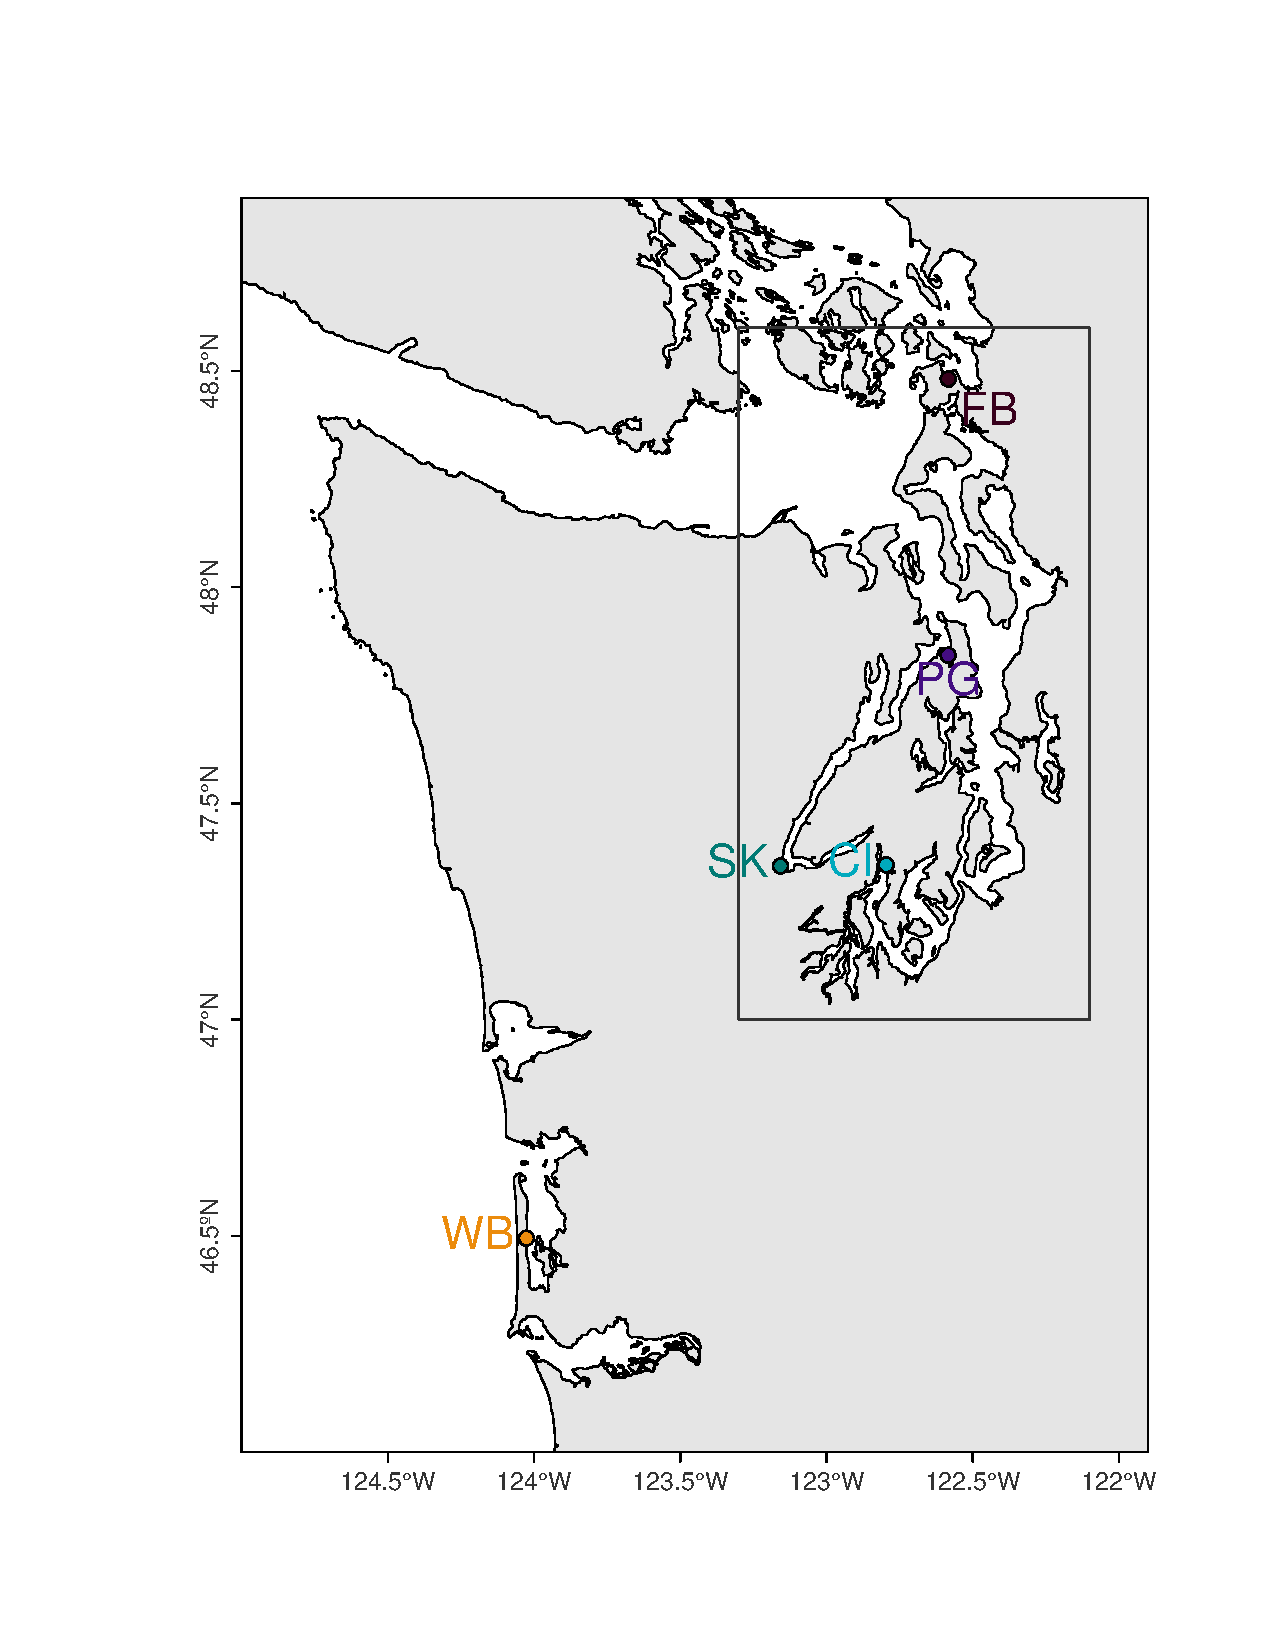
\includegraphics[width=0.65\textwidth]{figure/Ch1/fig1.1.pdf}
  \caption{Map of outplant sites}
  \label{fig:sitemap}
\end{figure}
\clearpage

\textbf{Figure} \ref{fig:envdatalines}: Environmental variables for each site (Case Inlet, Fidalgo Bay, Port Gamble Bay, Skokomish River Delta, and Willapa Bay) and habitat (unvegetated and eelgrass) over the course of the 29 day outplant.\newline
\begin{figure}[h]
  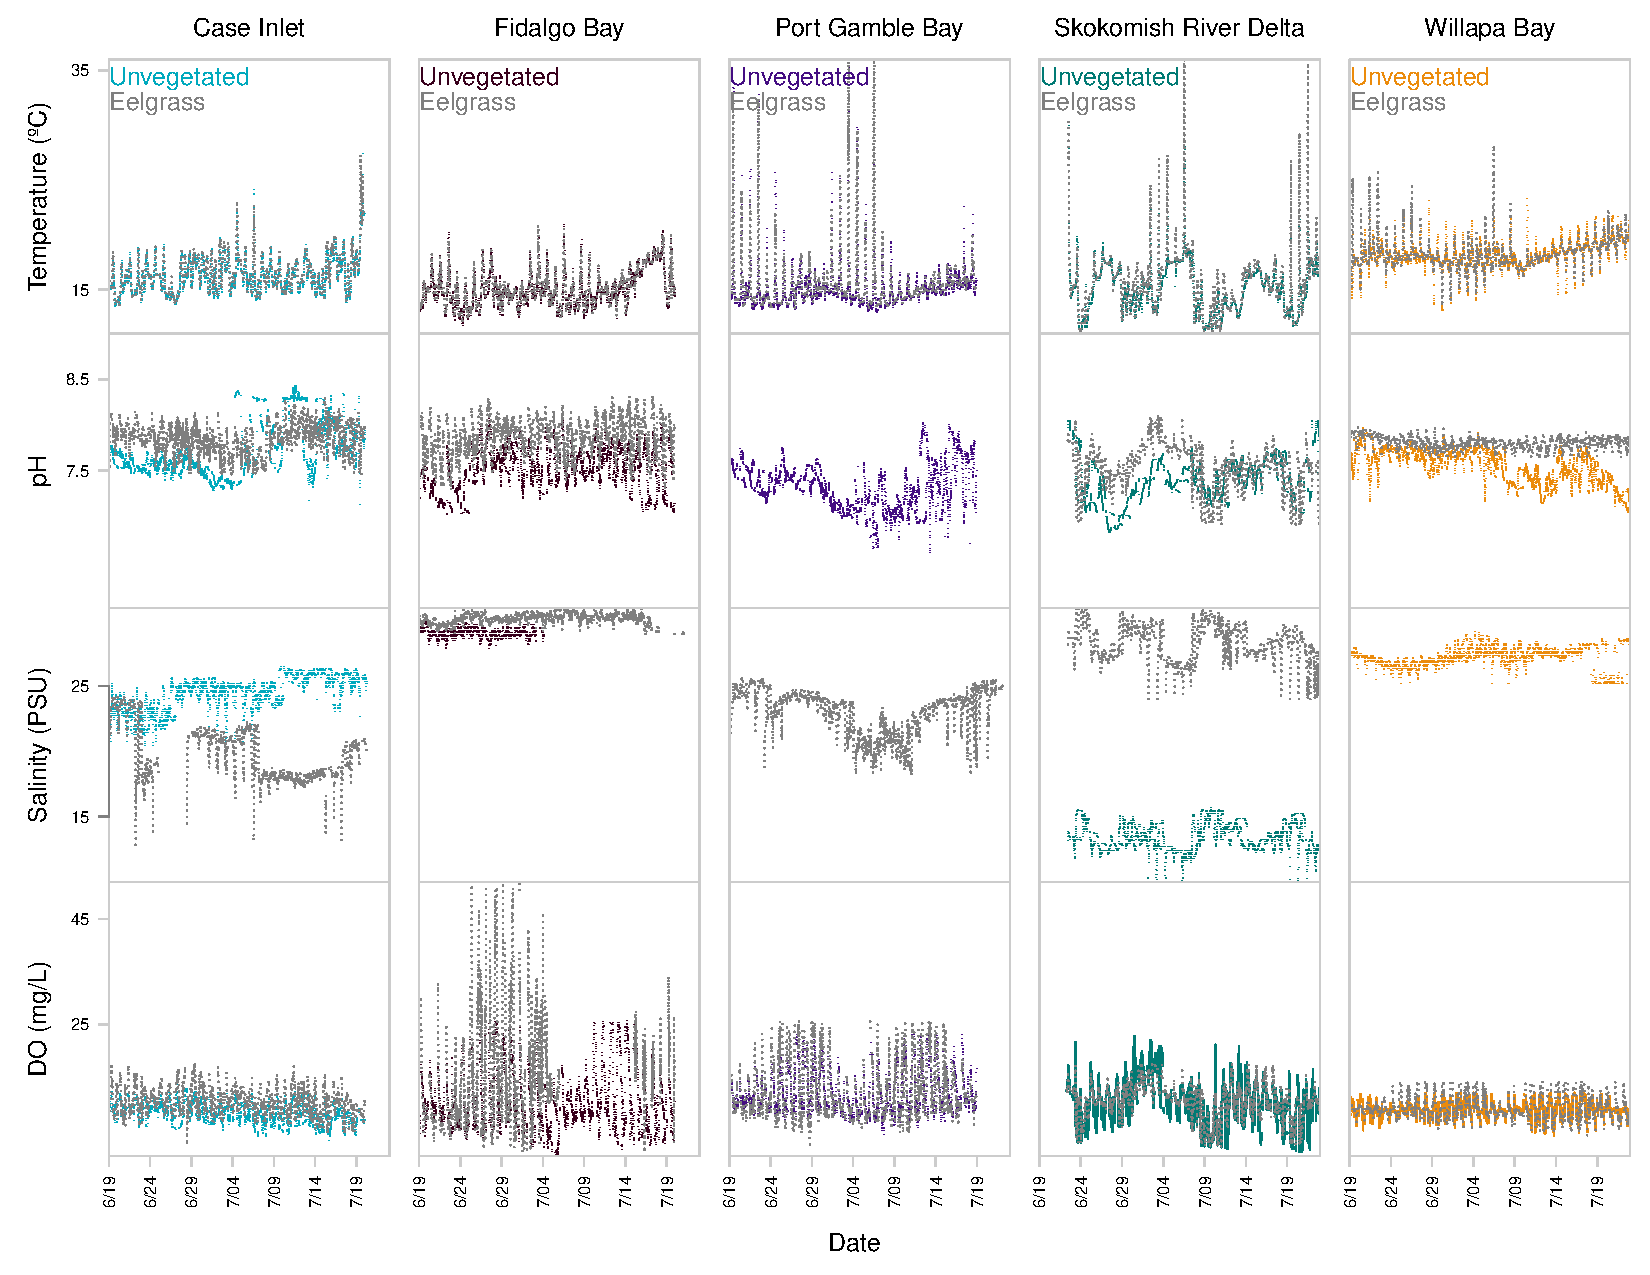
\includegraphics[width=1\textwidth]{figure/Ch1/fig1.2.pdf}
  \caption{Environmental data at each site}
  \label{fig:envdatalines}
\end{figure}
\clearpage

\textbf{Figure} \ref{fig:pepordination}: Ordination results for peptide abundance and environmental data. a) Environmental variables (pH, dissolved oxygen, salinity, and temperature) explained 30\% of variance in peptide abundance data; however, redundancy analysis (RDA) for peptide abundance constrained by environmental variable was not significant (ANOVA; F\textsubscript{6,19} = 1.306, p = 0.195). Temperature mean and variance were the most influential, yet nonsignificant, environmental predictors (ANOVA; temperature mean: F\textsubscript{1,25} = 2.3275, p = 0.065; temperature variance: F\textsubscript{1,25} = 2.1527, p = 0.067). Peptides differentially abundant between Fidalgo Bay (FB) and Willapa Bay (WB) are primarily positively loaded onto temperature mean, with two negatively loaded on temperature variance. b) Non-metric multidimensional scaling plot depicting peptide abundance by site and habitat, with 95\% confidence ellipses around each site (stress = 0.075, p = 0.0099). c) Peptides that contributed to significant peptide abundance differences between FB and WB, as determined by post-hoc similarity percentage analysis (SIMPER). Peptides denoted 1 correspond to peroxiredoxin-5 (PRX), 2 for carbonic anhydrase (CA), 3 for catalase (CAT), 4 for glucose-6-phosphate 1-dehydrogenase (G6PD), 5 for NADP transhydrogenase (NADPt), and 6 for protein disulfide isomerases 1 and 2 (PDI). FB peptide composition was differentiated by CA abundance, while all other proteins influenced peptide abundances at WB.\newline
\begin{figure}[h]
  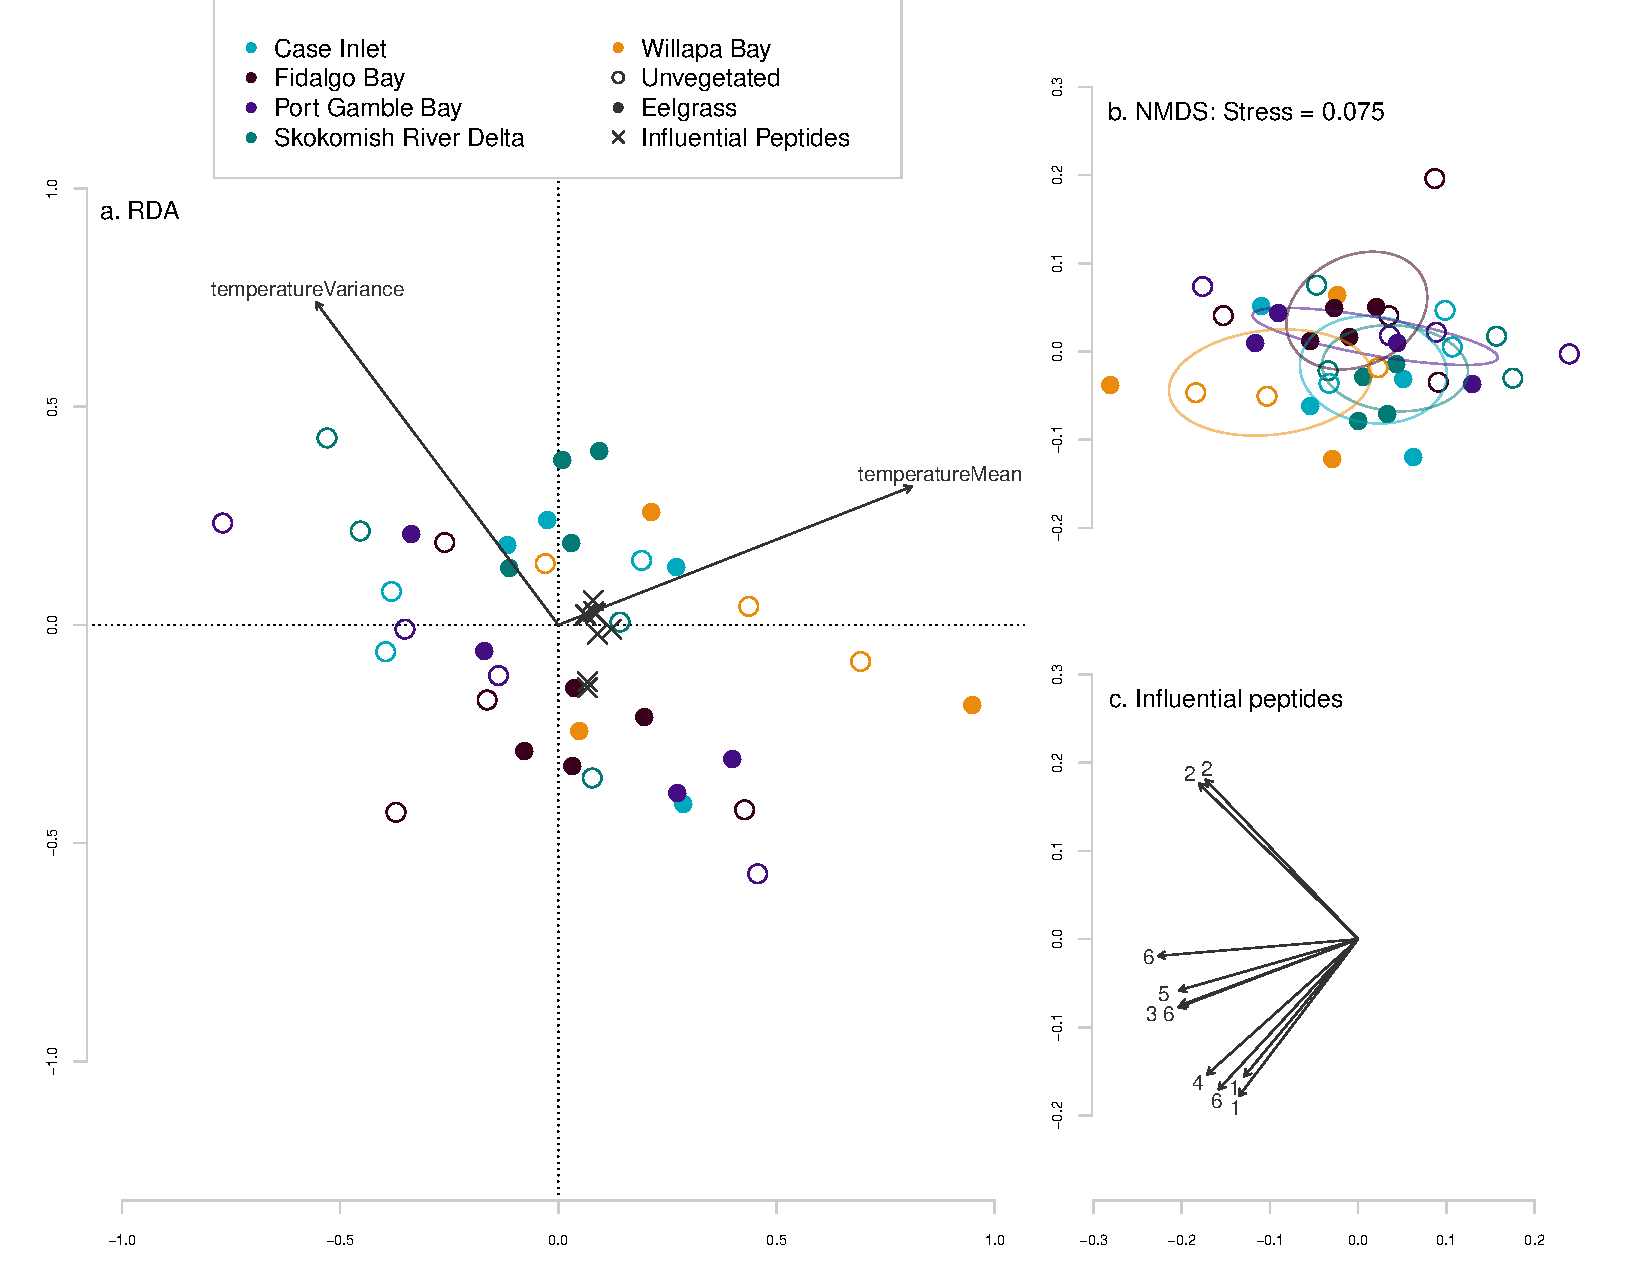
\includegraphics[width=1\textwidth]{figure/Ch1/fig1.3.pdf}
  \caption{Peptide abundance ordination results}
  \label{fig:pepordination}
\end{figure}
\clearpage

\textbf{Figure} \ref{fig:protheatmap}: Average protein abundance by constituent peptides across experimental sites from SRM. Peptide abundance data at each site was averaged, then log transformed. Proteins were considered differentially abundant if at least one constituent peptide was significantly different (indicated by an asterisk). There were no significant differences in protein abundance among the Puget Sound locations, or between unvegetated and eelgrass habitats. Proteins were only significantly different between Fidalgo Bay and Willapa Bay or Skokomish River Delta and Willapa Bay.\newline
\begin{figure}[h]
  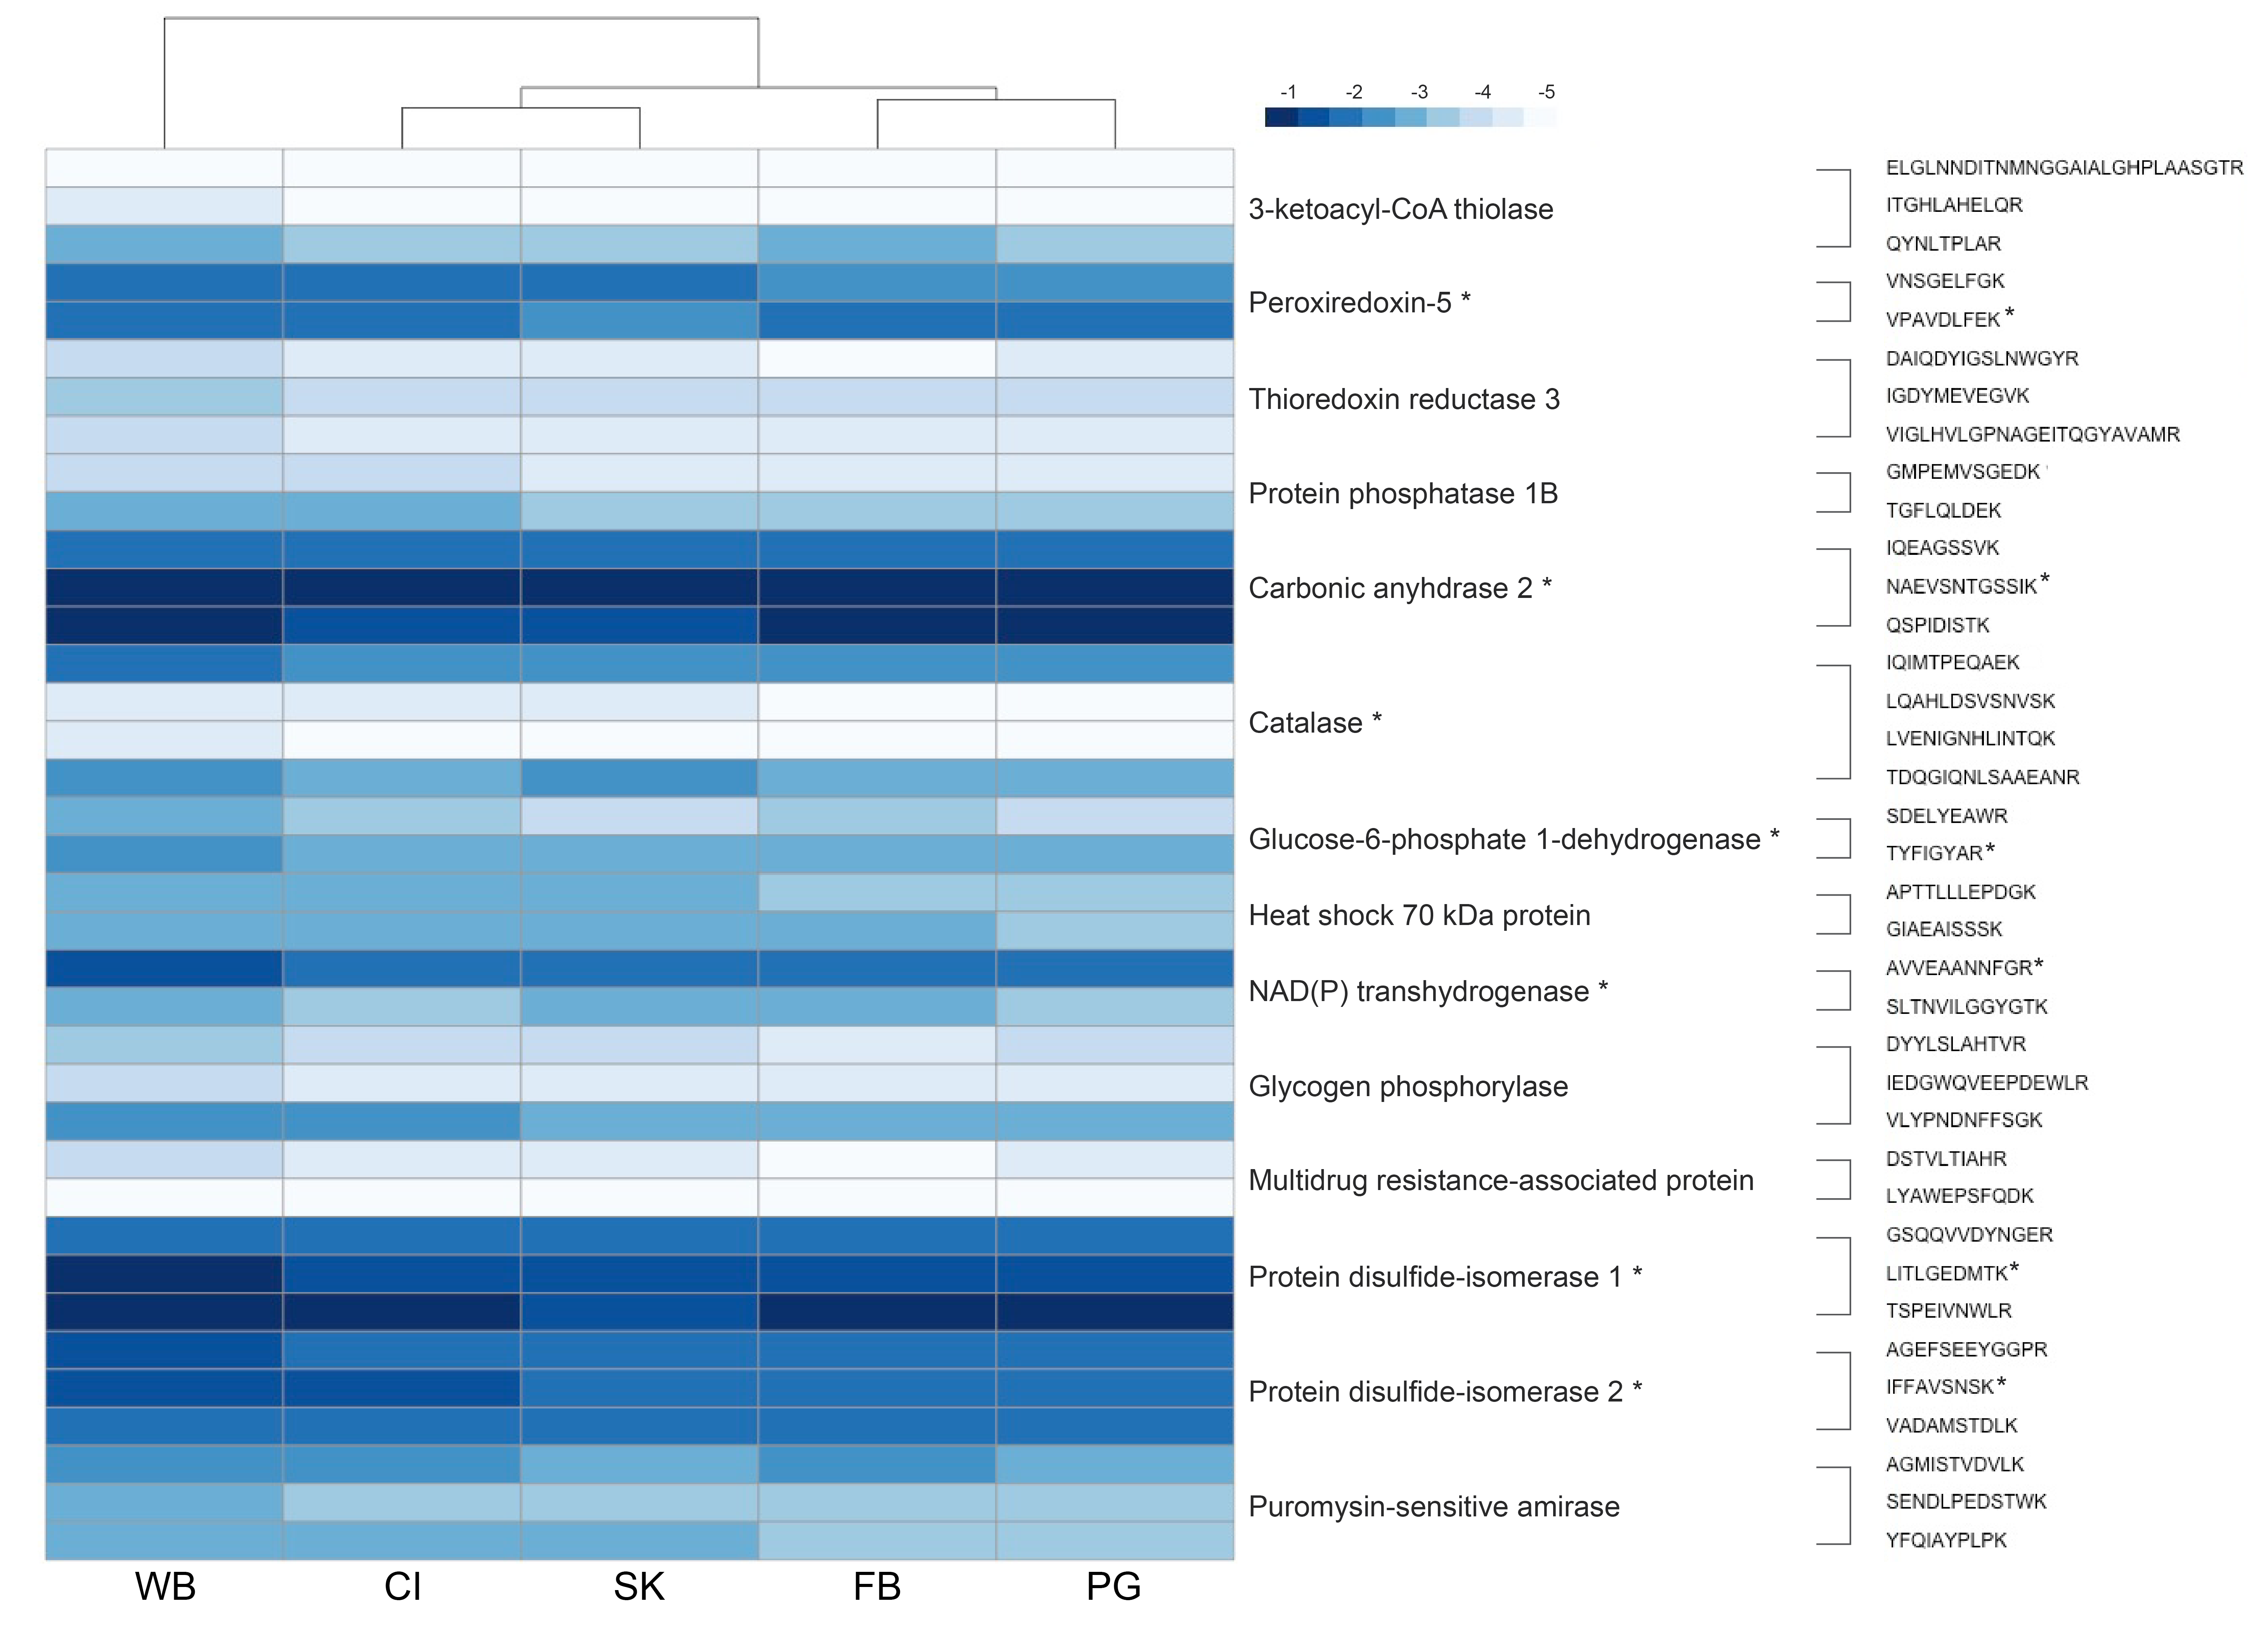
\includegraphics[width=1\textwidth]{figure/Ch1/fig1.4.png}
  \caption{Average protein abundance by site}
  \label{fig:protheatmap}
\end{figure}
\hypertarget{larval-response-to-parental-low-ph-exposure-in-pacific-oysters-crassostrea-gigas}{%
\chapter{\texorpdfstring{Larval response to parental low pH exposure in Pacific oysters (\emph{Crassostrea gigas})}{Larval response to parental low pH exposure in Pacific oysters (Crassostrea gigas)}}\label{larval-response-to-parental-low-ph-exposure-in-pacific-oysters-crassostrea-gigas}}

\hypertarget{abstract-1}{%
\section{Abstract}\label{abstract-1}}

As negative effects of ocean acidification are experienced by coastal ecosystems, there is a growing trend to investigate the effect ocean acidification has on multiple generations. Parental exposure to ocean acidification has been shown to induce larval carryover effects, but whether or not acute exposure to a stressor as an adult can influence the larval generation long after the stress has been removed has yet to be tested. To assess how a temporary exposure to experimental ocean acidification affects the ecologically and commercially relevant Pacific oyster (\emph{Crassostrea gigas}), adult oysters were exposed to either low pH (7.31 ± 0.02) or ambient pH (7.82 ± 0.02) conditions for seven weeks. Oysters were then held for eight weeks in ambient conditions, and subsequently reproductively conditioned for four weeks at ambient pH. After conditioning, oysters were strip-spawned to create four families based on maternal and paternal ocean acidification exposure. The number of D-hinge larvae were counted eighteen hours post-fertilization. A sex-specific broodstock response was observed, where female exposure to low pH conditions resulted in fewer D-hinge larvae. This study demonstrates that the effects of ocean acidification can last beyond the time from when the environmental perturbation is experienced. Broadening the understanding of environmental memory will be valuable when considering organismal ability to persist in the face of environmental change.

\hypertarget{introduction-2}{%
\section{Introduction}\label{introduction-2}}

Determining how parental exposure to ocean acidification carries over into early larval stages is important for understanding cumulative effects of climate-related environmental change. Gametogenesis is a key period during which parental exposure to ocean acidification can influence offspring (\protect\hyperlink{ref-Donelson2018}{\textbf{Donelson2018?}}). Several studies exposing Sydney rock oysters (\emph{Saccostrea glomerata}) to high pCO\textsubscript{2} conditions (856 µatm, pHNBS 7.89-7.90) during reproductive conditioning identified positive larval carryover effects (\protect\hyperlink{ref-Parker2012}{\textbf{Parker2012?}}; \protect\hyperlink{ref-Parker2015}{\textbf{Parker2015?}}; \protect\hyperlink{ref-Parker2017}{\textbf{Parker2017?}}). Specifically, larvae from parents exposed to low pH conditions were larger and developed faster in acidified conditions compared to those from parents reared in ambient pH conditions (\protect\hyperlink{ref-Parker2012}{\textbf{Parker2012?}}; \protect\hyperlink{ref-Parker2015}{\textbf{Parker2015?}}; \protect\hyperlink{ref-Parker2017}{\textbf{Parker2017?}}). Conversely, similar experiments conducted with northern quahog (= hard clam; \emph{Mercenaria mercenaria}) and bay scallops (\emph{Argopecten irradians}) demonstrated negative larval carryover effects (\protect\hyperlink{ref-Griffith2017}{\textbf{Griffith2017?}}). Larvae from adult \emph{A. irradians} and \emph{M. mercenaria} exposed to low pH were more sensitive to acidified conditions than those spawned from parents exposed to ambient pH during reproductive conditioning (\protect\hyperlink{ref-Griffith2017}{\textbf{Griffith2017?}}). These studies demonstrate the importance of parental exposure during reproductive conditioning (late-stage gametogenesis) on offspring.

As the Pacific oyster (\emph{Crassostrea gigas}; Thunberg, 1793) is a commercially and ecologically relevant species in much of the world, several research efforts have identified consequences of ocean acidification for distinct \emph{C. gigas} life stages. While fertilization still occurs under near-future ocean acidification conditions (\protect\hyperlink{ref-Kurihara2007}{Kurihara, Kato, \& Ishimatsu, 2007}; \protect\hyperlink{ref-Havenhand2009}{\textbf{Havenhand2009?}}; \protect\hyperlink{ref-Boulais2018}{\textbf{Boulais2018?}}), fertilization success in acidified conditions is variable between \emph{C. gigas} populations (\protect\hyperlink{ref-Parker2010}{\textbf{Parker2010?}}; \protect\hyperlink{ref-Barros2013}{\textbf{Barros2013?}}). Researchers have found that larvae experience developmental delays and reduced shell growth when exposed to experimental ocean acidification conditions (\protect\hyperlink{ref-Gazeau2011}{Gazeau et al., 2011}; \protect\hyperlink{ref-Kurihara2007}{Kurihara, Kato, \& Ishimatsu, 2007}; \protect\hyperlink{ref-Timmins-Schiffman2013}{Timmins-Schiffman, O'Donnell, Friedman, \& Roberts, 2013}; \protect\hyperlink{ref-Waldbusser2014}{Waldbusser et al., 2014}). Natural upwelling-induced ocean acidification conditions also reduced larval production and growth in a hatchery setting (\protect\hyperlink{ref-Barton2012}{\textbf{Barton2012?}}). Ocean acidification hampers protein expression in larvae, especially for proteins related to calcification and cytoskeleton production (\protect\hyperlink{ref-Dineshram2012}{\textbf{Dineshram2012?}}). During metamorphosis, oyster larvae experience down-regulation of proteins related to energy production, metabolism, and protein synthesis (\protect\hyperlink{ref-Dineshram2016}{Dineshram et al., 2016}). Adult \emph{C. gigas} calcification rates decrease as seawater pCO\textsubscript{2} increases (\protect\hyperlink{ref-Gazeau2007}{Gazeau et al., 2007}), with oysters grown at 2800 µatm displaying significantly lower fracture toughness than oyster shells from ambient conditions (\protect\hyperlink{ref-Timmins-Schiffman2014}{Timmins-Schiffman et al., 2014}). Exposure to ocean acidification also affects adult antioxidant responses, carbohydrate metabolism, transcription, and translation protein pathways (\protect\hyperlink{ref-Timmins-Schiffman2014}{Timmins-Schiffman et al., 2014}). Predator-prey interactions can also change under experimental ocean acidification (\protect\hyperlink{ref-Wright2018}{\textbf{Wright2018?}}). There is limited evidence, however, of how ocean acidification influences Pacific oysters across multiple generations.

The current study is the first to discern how exposure to experimental ocean acidification prior to reproductive conditioning affects larval abundance in \emph{C. gigas}. This experiment not only describes how isolated exposure to low pH during early gametogenesis influences larvae, but also provides information on the effects of acute pH exposure on adult gonad morphology. Additionally, the study demonstrates how environmental perturbation experienced before reproductive maturity affects the subsequent generation, even if the stressor is long-removed.

\hypertarget{methods-1}{%
\section{Methods}\label{methods-1}}

\hypertarget{experimental-overview}{%
\subsection{Experimental overview}\label{experimental-overview}}

Experimental trials were conducted at the Kenneth K. Chew Center for Shellfish Research and Restoration at the National Oceanic and Atmospheric Administration (NOAA) Manchester Field Station (47°34'09.1``N 122°33'19.0''W, Manchester, Washington, USA) in 2017. Adult hatchery-raised \emph{C. gigas} (average shell length = 117.46 ± 19.16 cm) were acclimated in the facility for 10 days, then exposed to either low or ambient pH conditions for 48 days (Figure 1). After pH exposure, oysters were held at ambient pH and water temperature conditions for 90 days. Oysters underwent reproductive conditioning for 22 days, then strip-spawned. D-hinge larvae were counted eighteen hours after fertilization occurred.

\hypertarget{experimental-ph-exposure}{%
\subsection{Experimental pH exposure}\label{experimental-ph-exposure}}

The experimental system consisted of a 1,610 liter storage tank that fed two 757 liter header tanks. Water from Clam Bay, WA was pumped through a sand filter, then UV-treated. The UV-treated water passed through a set of three sock filters (100 µm, 50 µm, and 25 µm) and a degassing column. Once degassed, water passed through three more sock filters (25 µm, then 10 µm, and 5 µm) before entering the storage tank. The storage tank was outfitted with an off-gas vent and pump to recirculate water such that CO\textsubscript{2} in the water could be equilibrated with atmospheric CO\textsubscript{2}. Equilibrated water flowed into the two header tanks, each of which fed three 50L flow-through (1.2 L/min) experimental tanks (six experimental tanks total). For all header and experimental tanks, pH in header and experimental tanks was continuously monitored using Durafet pH probes (Honeywell Model 51453503-505) and an AVTECH system. The addition of CO\textsubscript{2} in the low pH header tank was controlled using a solenoid valve. A Dual Input Analytical Analyzer (Honeywell Model 50003691-501) automatically mediated solenoid injections. A CO\textsubscript{2} airline with a back pressure of 15 psi, controlled with a regulator, injected CO\textsubscript{2} into the low pH header tank every 180 seconds with an injection duration of 0.4 seconds. Injections only occurred if real-time pH from the Durafet was above pH 7.22. A venturi injector connected to the ambient water line mixed ambient pH water with CO\textsubscript{2}-rich water to lower pH. There were no CO\textsubscript{2} injections in the ambient header tank.

Prior to the pH exposure trial, twenty randomly selected \emph{C. gigas} were lethally sampled to assess gonadal status (see \emph{Histological analysis}). Oysters were placed in each flow-through experimental tank in ambient water conditions and exposed to ambient or low pH conditions for seven weeks. Each treatment consisted of 3 tanks, each with 20 oysters. All experimental tanks received algae from a common reservoir. The algal tank contained 300-500 mL of Shellfish Diet 1800® (Reed Mariculture) diluted in 200L of ambient pH seawater (\protect\hyperlink{ref-Helm2004}{\textbf{Helm2004?}}). Algae was continuously dosed to oyster experimental tanks using an Iwaki Metering Pump. Algal lines were cleaned twice weekly, and experimental tanks were fully drained and cleaned once a week.

\hypertarget{seawater-chemistry-analysis}{%
\subsection{Seawater chemistry analysis}\label{seawater-chemistry-analysis}}

Twice a week, water samples (1L) were collected from each header and oyster experimental tank. For each sample, salinity was measured with a Bench/Portable Conductivity Meter (Model 23226-505, VWR), pH (mV) was measured with a Combination pH Electrode (Model 11278-220, Mettler Toledo), and temperature (ºC) was measured using a Traceable Digital Thermometer (Model 15-077, Fisher). To calibrate the pH probe, a Tris buffer (0.08 M, 28.0 salinity) was prepared using 0.3603 mol of NaCl (J.T. Baker), 0.0106 mol of KCl (Fisher Scientific), 0.0293 mol MgSO4-(H2O)7 (Fisher Scientific), 0.0107 mol of CaCl2-2(H2O) (MP Biomedicals), 0.0401 HCl (J.T. Baker), and 0.0799 mol of Tris base (Fisher Scientific). Deionized water was added for a final volume of 1L. Salinity, temperature, and pH measurements for the Tris buffer were obtained at five temperatures before measuring samples to generate a standard curve. This standard curve was used to calibrate the pH electrode and convert measured millivolts to pH units.

For total alkalinity measurements, duplicate seawater samples (250 mL) were collected from experimental tanks twice weekly and dosed with mercuric chloride (50 µL of 0.18 M solution) to preserve samples (\protect\hyperlink{ref-Bandstra2006}{\textbf{Bandstra2006?}}). Samples from days 5, 33, and 48 were run on a T5 Excellence titrator (Mettler Toledo) to determine alkalinity. Salinity from discrete samples was used to calculate total alkalinity, using the \texttt{seacarb} library in R (\protect\hyperlink{ref-Gattuso2018}{\textbf{Gattuso2018?}}). Calculated pH, total alkalinity, temperature, and salinity were also used in \texttt{seacarb} to calculate in situ pH, pCO\textsubscript{2}, dissolved organic carbon (DIC), calcite saturation (Ω\textsubscript{calcite}), and aragonite saturation (Ω\textsubscript{aragonite}) for days 5, 33, and 48. R code used to calculate water chemistry parameters is available in the \href{https://github.com/RobertsLab/paper-gigas-early-gametogenic-exposure}{Github repository}.

\hypertarget{histological-analysis}{%
\subsection{Histological analysis}\label{histological-analysis}}

Twenty randomly selected \emph{C. gigas} were lethally sampled before pH exposure for histological analyses. On the last day of low pH exposure, ten oysters from each treatment --- randomly selected from each tank --- were also lethally sampled to assess gonadal status. For each sampled oyster, a piece of gonad tissue was cut and placed in a histology cassette. Gonad tissue in cassettes was fixed for histology using PAXgene Tissue FIX and STABILIZER and sent to Diagnostic Pathology Medical Group, Inc.~(Sacramento, CA) for staining with hematoxylin and eosin and slide preparation. Tissues exposed to ambient pH were confounded during processing, preventing any tank identification. Maturation state and organism sex was evaluated histologically at 40x magnification (\protect\hyperlink{ref-Fabioux2005}{\textbf{Fabioux2005?}}; \protect\hyperlink{ref-Enruxedquez-Duxedaz2008}{\textbf{Enríquez-Díaz2008?}}).

\hypertarget{reproductive-conditioning}{%
\subsection{Reproductive conditioning}\label{reproductive-conditioning}}

Following seven weeks of low pH exposure, oysters were returned to a common garden and maintained at ambient pH conditions for eight weeks. Afterwards, oysters were reproductively conditioned. Water temperatures and food quantity are known to regulate the timing, speed, and intensity of gametogenesis in \emph{C. gigas} (\protect\hyperlink{ref-Enruxedquez-Duxedaz2008}{\textbf{Enríquez-Díaz2008?}}). Conditioning protocol was modeled after standard hatchery practices (Molly Jackson, Broodstock Manager at Taylor Shellfish, pers. comm., June 2017). Water temperature was raised from ambient conditions (13ºC) to 23ºC over three weeks (1ºC/2 days), since optimal temperature for \emph{C. gigas} gametogenesis is between 18ºC and 26ºC (\protect\hyperlink{ref-Parker2010}{\textbf{Parker2010?}}). Conditions were maintained at 23ºC for one more week prior to spawning. During conditioning, \emph{C. gigas} were fed 700-800 mL of Shellfish Diet 1800® daily (\protect\hyperlink{ref-Helm2004}{\textbf{Helm2004?}}).

\hypertarget{strip-spawning-and-larval-rearing}{%
\subsection{Strip spawning and larval rearing}\label{strip-spawning-and-larval-rearing}}

After reproductive conditioning, all surviving oysters were prepared for strip spawning. A sample of gonad from each individual was assessed for presence of active sperm or eggs using a microscope at 10x magnification. Only \emph{C. gigas} with active sperm or eggs were used for crosses (n\textasciitilde male, low\textasciitilde{} = 6, n\textasciitilde female, low\textasciitilde{} = 22, n\textasciitilde male, ambient\textasciitilde{} = 6, n\textasciitilde female, ambient\textasciitilde{} = 26). Presence of mature gametes and ripe oysters indicated that oysters were in good condition and not affected by use of Shellfish Diet 1800® instead of live algae during reproductive conditioning. For each treatment (low pH and ambient conditions), one gram of mature gonad from each ripe female was pooled. The number of eggs in both the ambient and low pH pools were counted to determine the number of eggs used for parental crosses. Parental crosses were created using 210,000 eggs from the female egg pools and sperm (200 µL) from individual males.

Four half-sibling families were created based on parental pH exposure: low pH female (pool) x low pH male, low pH female (pool) x ambient pH male, ambient pH female (pool) x low pH male, and ambient pH (pool) female x ambient pH male. These crosses were conducted using pooled eggs from either low pH or ambient pH females, and sperm from one of six males within each pH treatment (e.g.~low pH female pool x low pH male-01, low pH female pool x low pH male-02, \ldots{} low pH female pool x low pH male-06), totaling 24 crosses. All crosses were performed in duplicate, resulting in 48 separate fertilization events.

Fertilization was carried out in plastic beakers (1L) for 20 minutes with static 23ºC filtered seawater (1 µm) in ambient pH conditions. After confirming polar body formation, beaker contents were transferred to larger plastic tanks (19L) with aerated, static 23ºC filtered seawater (1 µm) for eighteen hours of incubation. Duplicate containers were combined eighteen hours post-fertilization, and D-hinge larvae were counted for each cross (n= 24).

\hypertarget{statistical-analyses}{%
\subsection{Statistical analyses}\label{statistical-analyses}}

Differences in in situ pH, total alkalinity, pCO\textsubscript{2}, DIC, Ω\textsubscript{calcite}, and Ω\textsubscript{aragonite} between pH treatments were evaluated with a one-way ANOVA. Because tissue samples were confounded during histological processing, a binomial GLM model was used to compare gonad maturation between pH treatments. Differences in sex ratios between pH treatments were evaluated using a chi-squared test of homogeneity. To identify differences in D-hinge larval counts, a linear mixed model was used, with sire and female egg pool as random effects. Differences in D-hinge larval counts by female treatment were assessed using a similar linear mixed model, with only sire as a random effect. Normality of data, as well as independence and homoscedasticity, were verified visually. All statistical analyses were carried out in R (Version 3.4.0). R Scripts are available in the supplementary \href{https://github.com/RobertsLab/paper-gigas-early-gametogenic-exposure}{Github repository}.

\hypertarget{results-1}{%
\section{Results}\label{results-1}}

\hypertarget{water-chemistry}{%
\subsection{Water chemistry}\label{water-chemistry}}

Pacific oysters exposed to low pH experienced different water chemistry parameters than those in the ambient pH treatment (Table 2.1). Using water samples from days 5, 33, and 48, pH (One-way ANOVA; F1, 16 = 5838.7810, p = 6.1165e-22), pCO\textsubscript{2} (One-way ANOVA; F\textasciitilde1, 16\textasciitilde{} = 235.4018, p = 5.4421e-11), DIC (One-way ANOVA; F\textasciitilde1, 16\textasciitilde{} = 7.1222, p = 0.0168), Ω\textsubscript{calcite} (One-way ANOVA; F\textasciitilde1, 16\textasciitilde{} = 528.9468, p = 1.0989e-13), Ω\textsubscript{aragonite} (One-way ANOVA; F\textasciitilde1, 16\textasciitilde{} = 526.5207, p =1.1389e-13) were significantly lower in the low pH treatment. Total alkalinity, however, was not significantly different between pH treatments (One-way ANOVA; F\textasciitilde1, 16\textasciitilde{} = F = 1.382, p = 0.2570).

\hypertarget{gonad-maturation}{%
\subsection{Gonad maturation}\label{gonad-maturation}}

A binomial GLM was used to compare gonad maturation of individuals sampled before and immediately after pH exposure, but before reproductive conditioning. The most parsimonious model included only sampling time (before or after pH treatment). Gonad maturation status was not significantly different between \emph{C. gigas} sampled before and after pH treatment (binomial GLM; F\textasciitilde2, 37\textasciitilde{} = 0.7973, p = 0.3442). Additionally, maturation status was not different between pH treatments (binomial GLM; F\textasciitilde3, 36\textasciitilde{} = 2.2675, p = 0.1408). No sampled oysters possessed fully mature gametes, but some males sampled appeared to be undergoing resorption (supplemental information available in the \href{https://github.com/RobertsLab/paper-gigas-early-gametogenic-exposure}{Github repository}). Sex ratios were also similar between low and ambient pH treatments (Chi-squared test for homogeneity; X\textsuperscript{2}\textsubscript{2} = 3.2279; p = 0.1942).

\hypertarget{larval-survival}{%
\subsection{Larval Survival}\label{larval-survival}}

A linear mixed effect model, with female pool and sire as random effects, demonstrated no significant difference in the number of D-hinge larvae counted eighteen hours post-fertilization between all four parental families (Linear mixed effect model; X\textsuperscript{2}\textsubscript{3} = 3.1325; p = 0.1066). Sire and female egg pools accounted for 0.8530\% and 3.1623\% of total variance, respectively. Significantly fewer D-hinge larvae were present in half-sibling families where females were exposed to low pH conditions (Figure 2; Linear mixed effect model; X\textsuperscript{2}\textsubscript{1} = 8.1781; p = 0.0042), with sire accounting for 0.3116053\% of total variance.

\hypertarget{discussion-1}{%
\section{Discussion}\label{discussion-1}}

The present study is the first to document the transgenerational influence of ocean acidification on Pacific oysters. Larval \emph{C. gigas} was negatively impacted when maternal broodstock were exposed to low pH (pH = 7.31), suggesting a maternal carryover effect. The experimental design of this study is also unique --- adult \emph{C. gigas} experienced low pH conditions three months prior to reproductive conditioning, then were kept solely in ambient pH conditions through strip spawning and larval rearing. Since environmental perturbation experienced before Pacific oysters were mature still affected larval oysters, the results indicate a role for environmental memory in \emph{C. gigas} response to ocean acidification. Mechanisms for transgenerational environmental memory have been explored in response to acute stressors in other species. For example, \emph{Daphnia magna} exposed to high salinity conditions had altered DNA methylation patterns, and these patterns were inherited by the following three non-exposed generations (\protect\hyperlink{ref-Jeremias2018}{\textbf{Jeremias2018?}}). Significant carryover effects observed in \emph{C. gigas} --- solely exposed to low pH when immature --- broaden the current understanding of stressor timing and its effect on organismal physiology.

While it is evident that acute exposure to low pH experienced by adult \emph{C. gigas} resulted in detrimental effects for larvae, the fact that larvae were not reared in acidified conditions makes cross-study comparison difficult. If \emph{C. gigas} larvae were also reared in acidified conditions, it is possible that larvae with a history of parental exposure to experimental ocean acidification may have exhibited a negative carryover effect on larval growth and performance. Negative carryover effects have been found in other marine invertebrate taxa, but all studies involved exposure to experimental ocean acidification during reproductive conditioning and larval rearing in acidified conditions. Tanner crabs (\emph{Chionoecetes bairdi}) solely exposed to acidified water (pH 7.5 or 7.8) as larvae did not exhibit significant changes in morphology, size, Ca/Mg content, or metabolic rate, yet substantial effects on physiology was observed when larvae had a history of maternal exposure during oogenesis (\protect\hyperlink{ref-Long2016}{\textbf{Long2016?}}). Larvae from adult northern quahog (= hard clam; \emph{M. mercenaria}) and bay scallops (\emph{A. irradians}) developed slower when parents were reproductively conditioned in low pH conditions (pH\textsubscript{T} = 7.4) (\protect\hyperlink{ref-Griffith2017}{\textbf{Griffith2017?}}). Additionally, larvae with a history of parental low pH exposure were more vulnerable to additional stressors like thermal stress, limited food, and harmful algae exposure (\protect\hyperlink{ref-Griffith2017}{\textbf{Griffith2017?}}). Although \emph{C. gigas} were not reproductively conditioned in acidified water, and the present study cannot distinguish between hatching success and early mortality, identifying a similar negative larval carryover effect four months after an acute environmental perturbation is arguably more surprising and significant, particularly in terms of efforts to understand the mechanism of environmental memory.

The severity of conditions experienced by organisms may also explain whether or not offspring demonstrate transgenerational acclimatization to stressors. For example, the negative carryover effect observed in \emph{C. gigas} is different from the positive carryover effects observed in ocean acidification experiments conducted with Sydney rock oysters. When adult \emph{S. glomerata} were exposed to acidified seawater (pCO\textsubscript{2} = 856 µatm; pH\textsubscript{NBS} = 7.89-7.90) during reproductive conditioning, resultant larvae were larger and developed faster in acidified conditions when compared to larvae from parents exposed to ambient conditions (\protect\hyperlink{ref-Parker2012}{\textbf{Parker2012?}}). This positive carryover effect was found to persist in the F2 generation. In acidified conditions, F2 offspring with a history of transgenerational (F0 and F1) pCO\textsubscript{2} exposure grew faster and demonstrated fewer shell abnormalities (\protect\hyperlink{ref-Parker2015}{\textbf{Parker2015?}}). While species-specific responses can certainly explain the observed differences in larval phenotypes, it is also likely that inconsistencies in treatment conditions between experiments resulted in dose-dependent effects. (\protect\hyperlink{ref-Parker2012}{\textbf{Parker2012?}}), (\protect\hyperlink{ref-Parker2015}{\textbf{Parker2015?}}), and (\protect\hyperlink{ref-Parker2017}{\textbf{Parker2017?}}) used a high pCO\textsubscript{2} treatment of 856 µatm (pH = 7.89-7.90), with a control of 380-385 µatm (pH = 8.19-8.20). Therefore, the elevated pCO\textsubscript{2} treatment used in those studies is similar to the ambient pH treatment (7.82; pCO\textsubscript{2} = 747.51-912.22) in the present study. Sydney rock oyster larvae with a history of transgenerational exposure exhibited faster development, but exhibited similar survival and were only 10\% larger in acidified conditions when compared to larvae with no transgenerational exposure history (\protect\hyperlink{ref-Parker2012}{\textbf{Parker2012?}}). With a relatively smaller effect size and a milder treatment than used in this study, it is possible these studies are not at odds but reflect dose-dependent effects on larval phenotypes. Negative carryover effects demonstrated in this study and in (\protect\hyperlink{ref-Griffith2017}{\textbf{Griffith2017?}}){]} can also be attributed to similar treatment pH levels (\protect\hyperlink{ref-Griffith2017}{\textbf{Griffith2017?}} pHT = 7.4, this study: pH = 7.31). Both of these studies used treatment levels more extreme than International Panel on Climate Change projections for open ocean acidification, but consistent with coastal and estuarine acidification scenarios experienced at study locations (\protect\hyperlink{ref-Feely2010}{\textbf{Feely2010?}}; \protect\hyperlink{ref-Griffith2017}{\textbf{Griffith2017?}}; \protect\hyperlink{ref-Pelletier2018}{\textbf{Pelletier2018?}}). More research is required to understand how location-specific conditions will affect multiple generations in a single species.

Although the effect of water chemistry on gametogenesis has been recorded in other taxa, it is unlikely that a low pH exposure occurring three months prior to reproductive conditioning could have affected gonad maturation. Studies in which reproductive conditioning and experimental ocean acidification occur concurrently have demonstrated negative effects on maturation and fecundity. Gametogenesis, especially oogenesis, was disrupted in eastern oysters (\emph{Crassostrea virginica}) that experienced severe ocean acidification conditions during reproductive conditioning (pH = 7.71, 5584 µatm) (\protect\hyperlink{ref-Boulais2017}{\textbf{Boulais2017?}}). Green sea urchins (\emph{Stronglyocentrotus droebachiensis}) exposed to high pCO\textsubscript{2} (1200 µatm) conditions for four months demonstrated low fecundity (\protect\hyperlink{ref-Dupont2013}{\textbf{Dupont2013?}}), and \emph{S. glomerata} conditioned in high pCO\textsubscript{2} (856 µatm) conditions exhibited reduced rates of gametogenesis, smaller gonad area, and reduced fecundity (\protect\hyperlink{ref-Parker2018}{\textbf{Parker2018?}}). Gonad histology from \emph{C. gigas} taken immediately after low or ambient pH exposure did not indicate any differences in maturation state, or interaction between sex and maturation state, between treatments. Even if fecundity or rates of gametogenesis differed between treatments, a return to ambient conditions for three months may have reversed any detrimental effects.

Reduced \emph{C. gigas} larval abundance could have been a result of altered maternal provisioning in female oysters exposed to low pH conditions. In the face of stressors, females can either increase maternal provisioning (\protect\hyperlink{ref-Allen2008}{\textbf{Allen2008?}}; \protect\hyperlink{ref-Sunday2011}{\textbf{Sunday2011?}}) --- diverting more resources, like lipids or proteins, into eggs --- or decrease provisioning due to energetic constraints (\protect\hyperlink{ref-Liu2010}{\textbf{Liu2010?}}; \protect\hyperlink{ref-Uthicke2013}{\textbf{Uthicke2013?}}). For example, changes in fatty acid provisioning from maternal exposure to high pCO\textsubscript{2} conditions (2300 µatm) in Atlantic silverside (\emph{Menidia menidia}) resulted in lower embryo survival when eggs lacked certain fatty acids (\protect\hyperlink{ref-Snyder2018}{\textbf{Snyder2018?}}). This phenomenon, however, was not documented in the Sydney rock oyster: while elevated pCO\textsubscript{2} conditions (856 µatm) reduced the amount of energy invested in maternal gonads, these conditions did not impact \emph{S. glomerata} egg size or total lipid content (\protect\hyperlink{ref-Parker2018}{\textbf{Parker2018?}}). Since adult \emph{C. gigas} did not experience environmental perturbation after low pH exposure, and received enough food to spawn well, any impact on maternal provisioning and subsequent larval abundance was likely a result of low pH three months prior to reproductive conditioning.

The documented effect on Pacific oyster larval abundance four months after low pH exposure indicates an important role for environmental memory in \emph{C. gigas} response to ocean acidification. Low pH exposure may have induced epigenetic modifications (eg. changes in DNA methylation) in adult \emph{C. gigas}. Studies of finfish and shellfish aquaculture species have demonstrated environmentally-induced epigenetic modifications that modify phenotypic responses in organisms (\protect\hyperlink{ref-Gavery2017}{Gavery \& Roberts, 2017}). One notable study on \emph{C. gigas} examined parental effects of adult pollutant exposure on offspring (\protect\hyperlink{ref-Rondon2017}{\textbf{Rondon2017?}}). Spat from parents exposed to the herbicide diuron had differential methylation in coding regions, with some changes leading to differential gene expression (\protect\hyperlink{ref-Rondon2017}{\textbf{Rondon2017?}}). This research indicates that a mechanism crucial for phenotypic plasticity and acclimation across generations exists, and this knowledge can be analyzed in the context of climate-related environmental stressors. Epigenetic modifications in response to ocean acidification have been documented in coral species (\protect\hyperlink{ref-Putnam2016}{\textbf{Putnam2016?}}), but not in molluscs. Several experimental ocean acidification studies, however, hint at the role of epigenetic memory. Olympia oysters (\emph{Ostrea lurida}) exposed to high pCO\textsubscript{2} (1000 µatm) conditions still grew less in the juvenile life stage than counterparts reared in ambient pCO\textsubscript{2}, even after the stressor had been removed (\protect\hyperlink{ref-Hettinger2013}{\textbf{Hettinger2013?}}). Similarly, transgenerational acclimation of \emph{S. glomerata} larvae with a history of exposure to acidified conditions could be explained by changes in epigenome that affect organismal performance (\protect\hyperlink{ref-Parker2012}{\textbf{Parker2012?}}; \protect\hyperlink{ref-Parker2015}{\textbf{Parker2015?}}; \protect\hyperlink{ref-Parker2017}{\textbf{Parker2017?}}). Methylation levels are known to increase over the course of gametogenesis, with male and female \emph{C. gigas} exhibiting significantly different methylation patterns (\protect\hyperlink{ref-Zhang2018}{\textbf{Zhang2018?}}). If epigenetic modifications were acquired by female oysters during low pH exposure, it could explain why a significant effect on larval abundance was detected four months after the exposure ended. Epigenetic mechanisms and altered maternal provisioning are not necessarily mutually exclusive --- changes in the methylome could influence maternal provisioning --- and both could contribute to the results observed in this study.

The results of this study emphasize the need to broaden the scope of when environmental perturbation experienced by an organism is considered stressful, and when an effect can be detected. Although there was no observable effect on adult gonad maturation right after low pH exposure, significant differences in larval abundance were detected four months after the exposure ended. Stressor timing and duration can impact transgenerational responses between mature parents and offspring (\protect\hyperlink{ref-Donelson2018}{\textbf{Donelson2018?}}). While experimental ocean acidification (pH 7.7; pCO\textsubscript{2} = 800 µatm) increased female investment in amphipods (\emph{Gammarus locusta}), the subsequent generation exhibited fewer eggs and lower fecundity in the same conditions (\protect\hyperlink{ref-Borges2018}{\textbf{Borges2018?}}). Transgenerational benefits of maternal exposure to different temperatures (17ºC or 21ºC) in threespine stickleback (\emph{Gasterosteus aculeatus}) differed based on exposure duration (\protect\hyperlink{ref-Shama2014}{\textbf{Shama2014?}}). Grandparents (F0) were only exposed to treatment temperatures during reproductive conditioning, while parents (F1) experienced either temperature over the course of development. The F1 generation exhibited temperature tolerances similar to the F0 maternal rearing environment, but the F2 generation tolerance was more similar to the F0 generation than the F1 generation (\protect\hyperlink{ref-Shama2014}{\textbf{Shama2014?}}). The present study demonstrates that length and timing of environmental perturbation experienced by immature individuals can still affect offspring. (\protect\hyperlink{ref-Massamba-N}{\textbf{Massamba-N?}})'Siala2014 elucidated a similar phenomenon with marine polychaetes (\emph{Ophryotocha labronica}): offspring experienced positive carryover effects of female exposure to temperature conditioning only when mothers were exposed to these conditions during late oogenesis; exposure during early oogenesis lead to negative carryover effects. More research should be conducted to understand how stressor timing, specifically before reproductive maturity, can impact carryover effects.

Most other experiments investigating stressor timing are conducted in a multiple stressor framework (\protect\hyperlink{ref-Gunderson2016}{\textbf{Gunderson2016?}}). For example, elevated temperatures and low salinity had synergistic effects on \emph{O. lurida} when they were co-occurring stressors, but two to four weeks of recovery in between stressors negated these effects (\protect\hyperlink{ref-Bible2017}{\textbf{Bible2017?}}). Incorporating recovery time in a single-stressor experimental design is also crucial for accurately understanding how environmental perturbation impacts organism physiology. Exposure at one point in time may elicit a response much later in time, in a different environmental setting, or in a different generation, as evidenced by the present study and (\protect\hyperlink{ref-Hettinger2013}{\textbf{Hettinger2013?}}). The experimental design in the present study is unique, featuring a significant recovery time between low pH exposure and spawning. More single-stressor experiments should incorporate lag times between exposure to stress and measuring response variables to understand if these responses change over time. Adding a multigenerational component to such experiments can elucidate if acute exposures generate carryover effects.

Significant decreases in larval abundance four months after broodstock were exposed to acidified seawater has implications for both aquaculture and natural \emph{C. gigas} populations. Parents and offspring --- or even different offspring life stages --- may not experience the same environmental chemistry. For example, upwelling conditions affecting adult \emph{C. gigas} may subside once spawning occurs. Long-term monitoring of wild Pacific oyster populations, with detailed environmental chemistry reporting, will be crucial for understanding how brief exposures to adverse conditions affect reproductive success and larval abundance in the field. Responses to stressors should not only be documented during and after the perturbation occurs, but also for an extended time afterward. Hatchery-reared \emph{C. gigas} larvae can also experience different conditions than broodstock. Facilities unable to control water chemistry conditions may be exposing immature individuals to environmental perturbations that could affect larvae once spawned. The success of ``priming'' --- exposing \emph{C. gigas} to stressful conditions to induce environmental memory and increase fitness --- hinges on the identification of ``programming windows'' (\protect\hyperlink{ref-Gavery2017}{Gavery \& Roberts, 2017}). The present study shows that the period of time before reproductive conditioning can be important for transferring environmental memory, although only negative carryover effects have been demonstrated in \emph{C. gigas}.

\clearpage

\hypertarget{tables-1}{%
\section{Tables}\label{tables-1}}
\begin{landscape}

Table 2.1: Average (± SE) pH, total alkalinity (µmol/kg), pCO~2~ (µatm), dissolved organic carbon (DIC; µmol/kg), calcite saturation state (Ω~calcite~), and aragonite saturation state (Ω~aragonite~) for three timepoints during low pH exposure (Day). The `seacarb` library in R was used to calculate total alkalinity, and in situ pCO~2~, Dissolved Inorganic Carbon (DIC), calcite saturation (Ω~calcite~), and aragonite saturation (Ω~aragonite~) for each oyster tank. Averages for both control (ambient pH) and experimental (low pH) values were calculated from three replicate tanks each. Between all three days, pH (One-way ANOVA; F~1, 16~ = 5838.7810, p = 6.1165e-22), pCO~2~ (One-way ANOVA; F~1, 16~ = 235.4018, p = 5.4421e-11), DIC (One-way ANOVA; F~1, 16~ = 7.1222, p = 0.0168), Ω~calcite~ (One-way ANOVA; F~1, 16~ = 528.9468, p = 1.0989e-13), Ω~aragonite~ (One-way ANOVA; F~1, 16~ = 526.5207, p =1.1389e-13) were significantly lower experimental treatment. Total alkalinity, however, was not significantly different between treatments (One-way ANOVA; F~1, 16~ = 1.382, p = 0.2570).


```
Warning in read.table(file = file, header = header, sep = sep, quote = quote, :
incomplete final line found by readTableHeader on 'data/Ch2/Table2.1.csv'
```

\begingroup\fontsize{10}{12}\selectfont
\begin{longtable}[t]{rllllllllllll}
\caption{\label{tab:carbchem}Carbonate chemistry parameters}\\
\toprule
Day & C pH & E pH & C Total Alkalinity & E Total Alkalinity & C pCO2 & E pCO2 & C  DIC & E DIC & C Calcite & E Calcite & C Aragonite & E Aragonite\\
\midrule
5 & 7.82 ± 0.004 & 7.33 ± 0.002 & 2307.41 ± 25.45 & 2332.36 ± 31.05 & 747.51 ± 13.94 & 2481.23 ± 29.83 & 2233.41 ± 25.29 & 2408.51 ± 31.76 & 1.86 ± 0.02 & 0.62 ± 0.01 & 1.16 ± 0.012  & 0.58 ± 0.007\\
33 & 7.81 ± 0.005 & 7.31 ± 0.004 & 2747.00 ± 21.13 & 2917.60 ± 18.36 & 912.22 ± 12.69 & 3309.52 ± 7.22 & 2664.57 ± 19.99 & 3020.99 ± 17.99 & 2.23 ± 0.03 & 0.77 ± 0.02 & 1.40 ± 0.020 & 0.48 ± 0.014\\
48 & 7.82 ± 0.015 & 7.29 ± 0.004 & 2611.40 ± 31.01 & 2808.39 ± 12.24 & 863.47 ± 42.42 & 3343.89 ± 49.49 & 2533.28 ± 35.45 & 2920.52 ± 15.11 & 2.13 ± 0.06 & 0.68 ± 0.01 & 1.32 ± 0.035 & 0.42 ± 0.004\\
\bottomrule
\end{longtable}
\endgroup{}

\end{landscape}
\clearpage

\#\#Figures
\begin{landscape}

Figure 2.1: Mechanisms of environmentally induced changes in resources (A-D) assimilated into stable isotope ratios of primary producers (1-2), which are conserved when assimilated into higher trophic levels in the food web (3).\newline 
\begin{figure}[h]
\centering
  \includegraphics[width=1.1\textwidth]{figure/Ch2/Figure1.pdf}
  \caption{Mechanisms of stable isotope change}
  \label{fig:theo}
\end{figure}
\end{landscape}
\clearpage

\textbf{Figure} \ref{fig:map}: Spatial and temporal distributions of northeast Pacific harbor seal specimens by subregion analyzed for \(\delta^{15}N_{Phe}\) and bulk \(\delta^{13}C\) values. Subplot colors correspond to map locations and x-axis (years) is the same for each subplot.\newline 
\begin{figure}[h]
\centering
  \includegraphics[width=1.2\textwidth]{figure/Ch2/Fig2_Map.pdf}
  \caption{Distribution of harbor seal specimens}
  \label{fig:map}
\end{figure}
\clearpage

\textbf{Figure} \ref{fig:dist}: Variability in \(\delta^{15}N_{Phe}\) and \(\delta^{13}C\) values based on sub region and sex. * denotes a significant difference in isotopic signature between males and females for that region (colors correspond to \ref{fig:map}).
\newline 
\begin{figure}[h]
\centering
  \includegraphics[width=1\textwidth]{figure/Ch2/Figure3_SexLocation.pdf}
  \caption{Distribution of harbor seal specimens}
  \label{fig:dist}
\end{figure}
\clearpage

\textbf{Figure} \ref{fig:hiermod}: Relationship between nitrogen sources (\(\delta^{15}N_{Phe}\)) and primary production (\(\delta^{13}C\)) assimilated into the food web for A. a single linear model for the combined data across the northeast Pacific and eastern Bering Sea and B. a mixed effects model with random slope and intercept by sub region (colors correspond to \ref{fig:map}).
\newline 
\begin{figure}[h]
\centering
  \includegraphics[width=1\textwidth]{figure/Ch2/hiermod.pdf}
  \caption{Hierarchical $\delta^{15}N_{Phe}$ and $\delta^{13}C$ Models}
  \label{fig:hiermod}
\end{figure}
\clearpage

\textbf{Figure} \ref{fig:coefres}: Coefficients of environmental covariates for models with relative support (\(\Delta AIC_c\) \textless{} 2) for harbor seal \(\delta^{15}N_{Phe}\) and \(\delta^{13}C\) values in three regions of the northeast Pacific: Washington, Gulf of Alaska, and the eastern Bering Sea. Color indicates model support based on AIC\textsubscript{c} weight, points are the coefficient estimates for each environmental covariate included in an individual model, and bars show two standard deviations from the coefficient estimate.
\newline 
\begin{figure}[h]
\centering
  \includegraphics[width=0.9\textwidth]{figure/Ch2/Figure5_CoefPlot.pdf}
  \caption{Coefficients of Evironmental Covariates}
  \label{fig:coefres}
\end{figure}
\clearpage

\textbf{Figure} \ref{fig:GDFAAK}: Common trends in environmental condition and food web assimilated stable isotope values for the regional Gulf of Alaska gaussian-dynamic factor analysis model. The solid lines represent the modelled trends, where 0 is the long-term average and 1 and -1 represent the maximum and minimum possible values respectively; the dash line is the 90\% credible interval. Factor loadings can be interpreted as coefficients, representing the strength of association between the modelled trend and each observed environmental time series (colors represent a priori driver category). Values close to 0 mean the observed time series did not correlate to the corresponding trend, while values close to 1 show the observed time series closely matched the modelled trend. Negative loadings indicate an inverse relationship between the observed time series and modelled trend. Stable isotope times series are modelled separately for the northern (N. \(\delta^{15}N_{Phe}\); N. \(\delta^{13}C\)) and southeast (S. \(\delta^{15}N_{Phe}\); S. \(\delta^{13}C\)) subregions.\\
\newline 
\begin{figure}[h]
\centering
  \includegraphics[width=0.9\textwidth]{figure/Ch2/Figure6_AK.GDFA.pdf}
  \caption{Alaska GDFA Results}
  \label{fig:GDFAAK}
\end{figure}
\clearpage

\textbf{Figure} \ref{fig:GDFAWA}: Common trends in environmental condition and food web assimilated stable isotope values for the regional Washington gaussian-dynamic factor analysis model. Stable isotope times series are modelled separately for the coastal (C. \(\delta^{15}N_{Phe}\); C. \(\delta^{13}C\)) and Salish Sea (S.S. \(\delta^{15}N_{Phe}\); S.S. \(\delta^{13}C\)) subregions. See \ref{fig:GDFAAK} caption for further interpretation.\\
\newline 
\begin{figure}[h]
\centering
  \includegraphics[width=0.9\textwidth]{figure/Ch2/Figure7_WA.GDFA.pdf}
  \caption{Washington GDFA Results}
  \label{fig:GDFAWA}
\end{figure}
\clearpage

\textbf{Figure} \ref{fig:Month}: Analysis of a) \(\delta^{15}N_{Phe}\) and b) \(\delta^{13}C\) values by month. For both models, s(month) p \textgreater{} 0.1 indicating no seasonality of harbor seal bone collagen stable isotope signature.\\
\newline 
\begin{figure}[h]
  \centering
  \includegraphics[width=0.8\textwidth]{figure/Ch2/figures2.png}
  \caption{Bone collagen stable isotope seasonality analysis}
  \label{fig:Month}
\end{figure}
\clearpage

\textbf{Figure} \ref{fig:Length}: Analysis of a) \(\delta^{15}N_{Phe}\) and b) \(\delta^{13}C\) values by length. For both models, there was no significant slope (p\textgreater0.1)
\newline 
\begin{figure}[h]
\centering
  \includegraphics[width=0.8\textwidth]{figure/Ch2/FigureS2.pdf}
  \caption{Bone collagen stable isotope length analysis}
  \label{fig:Length}
\end{figure}
\clearpage

\textbf{Figure} \ref{fig:TSphe}: Bone collagen \(\delta^{15}N\) values of phenylalanine from archival harbor seal specimens collected in the northeastern Pacific in five subregions.
\newline 
\begin{figure}[h]
\centering
  \includegraphics[height=0.8\textwidth]{figure/Ch2/FigureS3.pdf}
  \caption{Time series of $\delta^{15}N_{Phe}$ data}
  \label{fig:TSphe}
\end{figure}
\clearpage

\textbf{Figure} \ref{fig:nonSuess}: Bone collagen bulk \(\delta^{13}C\) values of archival harbor seal specimens collected in the northeastern Pacific in five subregions.These values are not corrected for the Suess effect.
\newline 
\begin{figure}[h]
\centering
  \includegraphics[height=0.8\textwidth]{figure/Ch2/FigureS4.pdf}
  \caption{Time series of $\delta^{13}C$ data}
  \label{fig:nonSuess}
\end{figure}
\clearpage

\textbf{Figure} \ref{fig:Suess}: Bone collagen bulk \(\delta^{13}C\) values of archival harbor seal specimens collected in the northeastern Pacific in five subregions.These values are corrected for the Seuss effect.
\newline 
\begin{figure}[h]
\centering
  \includegraphics[height=0.8\textwidth]{figure/Ch2/FigureS5.pdf}
  \caption{Time series of $\delta^{13}C$ data corrected for Suess effect}
  \label{fig:Suess}
\end{figure}
\clearpage

\textbf{Figure} \ref{fig:bulkN}: Bone collagen bulk \(\delta^{15}N\) values of archival harbor seal specimens collected in the
northeastern Pacific in five subregions.
\newline 
\begin{figure}[h]
\centering
  \includegraphics[height=0.8\textwidth]{figure/Ch2/FigureS6.pdf}
  \caption{Time series of bulk $\delta^{15}N$ data}
  \label{fig:bulkN}
\end{figure}
\clearpage

\textbf{Figure} \ref{fig:linresid}: Residuals for the model with the most support (\ref{fig:coefres}) plotted by year. A trend in model residuals would indicate environmental variables do not account for all temporal variation in harbor seal \(\delta^{15}N_{Phe}\) and \(\delta^{13}C\) values.
\newline 
\begin{figure}[h]
\centering
  \includegraphics[height=0.85\textwidth]{figure/Ch2/FigureS7.pdf}
  \caption{Residuals trends for linear models with the most support}
  \label{fig:linresid}
\end{figure}
\clearpage

Figure 2.15: Model residual plots for the models with the most support from the candidate model set. Note: EBS phenylalanine is an intercept only model, GOA phenylalanine only contains a 2-factor location as a covariate.
\newline 
\begin{figure}[h]
\centering
  \includegraphics[height=0.8\textwidth]{figure/Ch2/FigureS8.pdf}
  \caption{Residuals for linear models with the most support}
  \label{fig:linresid2}
\end{figure}
\hypertarget{ref-labels}{%
\chapter{Tables, Graphics, References, and Labels}\label{ref-labels}}

\hypertarget{tables}{%
\section{Tables}\label{tables}}

By far the easiest way to present tables in your thesis is to store the contents of the table in a CSV or Excel file, then read that file in to your R Markdown document as a data frame. Then you can style the table with the \texttt{kable} function, or functions in the \href{https://cran.r-project.org/web/packages/kableExtra/index.html}{kableExtra} pacakge.

In addition to the tables that can be automatically generated from a data frame in \textbf{R} that you saw in {[}R Markdown Basics{]} using the \texttt{kable} function, you can also create tables using \emph{pandoc}. (More information is available at \url{http://pandoc.org/README.html\#tables}.) This might be useful if you don't have values specifically stored in \textbf{R}, but you'd like to display them in table form. Below is an example. Pay careful attention to the alignment in the table and hyphens to create the rows and columns. Generally I don't recommend this approach of typing the table directly into your R Markdown document.
\begin{longtable}[]{@{}
  >{\centering\arraybackslash}p{(\columnwidth - 4\tabcolsep) * \real{0.31}}
  >{\centering\arraybackslash}p{(\columnwidth - 4\tabcolsep) * \real{0.51}}
  >{\centering\arraybackslash}p{(\columnwidth - 4\tabcolsep) * \real{0.18}}@{}}
\caption{\label{tab:inher} Correlation of Inheritance Factors for Parents and Child}\tabularnewline
\toprule
Factors & Correlation between Parents \& Child & Inherited \\
\midrule
\endfirsthead
\toprule
Factors & Correlation between Parents \& Child & Inherited \\
\midrule
\endhead
Education & -0.49 & Yes \\
Socio-Economic Status & 0.28 & Slight \\
Income & 0.08 & No \\
Family Size & 0.18 & Slight \\
Occupational Prestige & 0.21 & Slight \\
\bottomrule
\end{longtable}
We can also create a link to the table by doing the following: Table \ref{tab:inher}. If you go back to {[}Loading and exploring data{]} and look at the \texttt{kable} table, we can create a reference to this max delays table too: Table \ref{tab:maxdelays}. The addition of the \texttt{(\textbackslash{}\#tab:inher)} option to the end of the table caption allows us to then make a reference to Table \texttt{\textbackslash{}@ref(tab:label)}. Note that this reference could appear anywhere throughout the document after the table has appeared.

\clearpage

\hypertarget{figures-1}{%
\section{Figures}\label{figures-1}}

If your thesis has a lot of figures, \emph{R Markdown} might behave better for you than that other word processor. One perk is that it will automatically number the figures accordingly in each chapter. You'll also be able to create a label for each figure, add a caption, and then reference the figure in a way similar to what we saw with tables earlier. If you label your figures, you can move the figures around and \emph{R Markdown} will automatically adjust the numbering for you. No need for you to remember! So that you don't have to get too far into LaTeX to do this, a couple \textbf{R} functions have been created for you to assist. You'll see their use below.

In the \textbf{R} chunk below, we will load in a picture stored as \texttt{uw.png} in our main directory. We then give it the caption of ``UW logo,'' the label of ``uwlogo,'' and specify that this is a figure. Make note of the different \textbf{R} chunk options that are given in the R Markdown file (not shown in the knitted document).
\begin{Shaded}
\begin{Highlighting}[]
\NormalTok{knitr}\SpecialCharTok{::}\FunctionTok{include\_graphics}\NormalTok{(}\AttributeTok{path =} \StringTok{"figure/uw.png"}\NormalTok{)}
\end{Highlighting}
\end{Shaded}
\begin{figure}
\includegraphics[width=6.25in]{figure/uw} \caption{UW logo}\label{fig:uwlogo}
\end{figure}
Here is a reference to the UW logo: Figure \ref{fig:uwlogo}. Note the use of the \texttt{fig:} code here. By naming the \textbf{R} chunk that contains the figure, we can then reference that figure later as done in the first sentence here. We can also specify the caption for the figure via the R chunk option \texttt{fig.cap}.

\clearpage

Below we will investigate how to save the output of an \textbf{R} plot and label it in a way similar to that done above. Recall the \texttt{flights} dataset from Chapter \ref{rmd-basics}. (Note that we've shown a different way to reference a section or chapter here.) We will next explore a bar graph with the mean flight departure delays by airline from Portland for 2014. Note also the use of the \texttt{scale} parameter which is discussed on the next page.
\begin{Shaded}
\begin{Highlighting}[]
\NormalTok{flights }\SpecialCharTok{\%\textgreater{}\%} \FunctionTok{group\_by}\NormalTok{(carrier) }\SpecialCharTok{\%\textgreater{}\%}
  \FunctionTok{summarize}\NormalTok{(}\AttributeTok{mean\_dep\_delay =} \FunctionTok{mean}\NormalTok{(dep\_delay)) }\SpecialCharTok{\%\textgreater{}\%}
  \FunctionTok{ggplot}\NormalTok{(}\FunctionTok{aes}\NormalTok{(}\AttributeTok{x =}\NormalTok{ carrier, }\AttributeTok{y =}\NormalTok{ mean\_dep\_delay)) }\SpecialCharTok{+}
  \FunctionTok{geom\_bar}\NormalTok{(}\AttributeTok{position =} \StringTok{"identity"}\NormalTok{, }\AttributeTok{stat =} \StringTok{"identity"}\NormalTok{, }\AttributeTok{fill =} \StringTok{"red"}\NormalTok{)}
\end{Highlighting}
\end{Shaded}
\begin{figure}
\centering
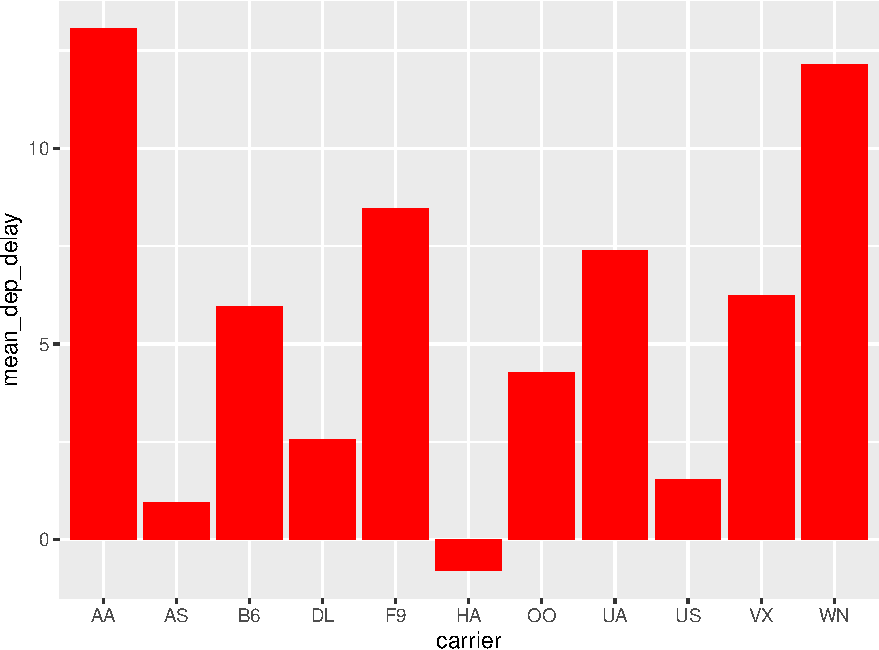
\includegraphics{thesis_files/figure-latex/delaysboxplot-1.pdf}
\caption{\label{fig:delaysboxplot}Mean Delays by Airline}
\end{figure}
Here is a reference to this image: Figure \ref{fig:delaysboxplot}.

A table linking these carrier codes to airline names is available at \url{https://github.com/ismayc/pnwflights14/blob/master/data/airlines.csv}.

\clearpage

Next, we will explore the use of the \texttt{out.extra} chunk option, which can be used to shrink or expand an image loaded from a file by specifying \texttt{"scale=\ "}. Here we use the mathematical graph stored in the ``subdivision.pdf'' file.
\begin{figure}
\includegraphics[scale=0.75]{figure/subdivision} \caption{Subdiv. graph}\label{fig:subd}
\end{figure}
Here is a reference to this image: Figure \ref{fig:subd}. Note that \texttt{echo=FALSE} is specified so that the \textbf{R} code is hidden in the document.

\textbf{More Figure Stuff}

Lastly, we will explore how to rotate and enlarge figures using the \texttt{out.extra} chunk option. (Currently this only works in the PDF version of the book.)
\begin{figure}
\includegraphics[angle=180, scale=1.1]{figure/subdivision} \caption{A Larger Figure, Flipped Upside Down}\label{fig:subd2}
\end{figure}
As another example, here is a reference: Figure \ref{fig:subd2}.

\hypertarget{footnotes-and-endnotes}{%
\section{Footnotes and Endnotes}\label{footnotes-and-endnotes}}

You might want to footnote something.\footnote{footnote text} The footnote will be in a smaller font and placed appropriately. Endnotes work in much the same way.

\hypertarget{cross-referencing-chapters-and-sections}{%
\section{Cross-referencing chapters and sections}\label{cross-referencing-chapters-and-sections}}

The \href{https://bookdown.org/yihui/bookdown/cross-references.html}{bookdown documentation} is an excellent source for learning how to cross-reference in a bookdown project such as a huskydown document. Here we only cover the most common uses for a typical thesis. If you want something more complex or fancy, please refer to the bookdown documentation and seek help from the developers of that package.

By default, all of your chapter and section headers will get an auto-generated ID label For example, e.g., \texttt{\#\ Chapter\ 1} will have an auto-generated ID \texttt{chapter-1}. Note that the ID label is all lower case, and has no spaces. If you have any kind of punctuation in your header, such as a colon (:), it will not appear in the ID label. Then in your text you can reference chapter one in your Rmd file like this: `as discussed in Chapter \texttt{\textbackslash{}@ref(chapter-1)},' which will print as `as discussed in Chapter 1'

We strongly recommend that you to manually assign ID labels to your chapter header to make it easy to cross-reference. For example, at the top of the Rmd file for this chapter, you can see:

\texttt{\#\ Tables,\ Graphics,\ References,\ and\ Labels\ \{\#ref-labels\}}

The \texttt{\{\#ref-labels\}} part of this header is the ID label. It doesn't show in the output, but is there for us to use for easy cross-referencing, because it can be short, and we don't need to change it elsewhere our document when we update the chapter header. We can use this custom ID label in our Rmd document like this: `as discussed in Chapter \texttt{\textbackslash{}@ref(ref-labels)},' which will print as `as discussed in Chapter \ref{ref-labels}.' If you need to show custom text instead of the chapter number, you use this syntax in your Rmd document: \texttt{see\ {[}my\ chapter\ about\ labels{]}(\#ref-labels)\ for\ more\ details} which will appear as `see \protect\hyperlink{ref-labels}{my chapter about labels} for more details'

To cross-reference a specific section in the same chapter, we recommend adding a custom ID label to the section header, and using that to cross-reference. For example, earlier in this chapter we have a section on tables and in the Rmd file we see \texttt{\#\#\ Tables\ \{\#tables\}}. We can cross-reference that in the text like this `as discussed in the section on \texttt{{[}tables{]}(\#tables)}' which will appear as `as discussed in the above section on \protect\hyperlink{tables}{tables}'

To cross-reference a section in a different chapter we can use the ID label from that section directly. For example, we can write in our Rmd document \texttt{as\ discussed\ in\ the\ section\ on\ {[}R\ code\ chunks{]}(\#r-chunks)\ in\ Chapter\ \textbackslash{}@ref(rmd-basics)} which will appear as `as discussed in the section on \protect\hyperlink{r-chunks}{R code chunks} in Chapter \ref{rmd-basics}.'

If you prefer to cross-reference by the section number, we can use custom ID labels in our Rmd document. For example, to refer to a section in our first chapter, we can write in the Rmd document: \texttt{as\ discussed\ in\ section\ \textbackslash{}@ref(r-chunks)\ in\ Chapter\ \textbackslash{}@ref(rmd-basics)}. This will appear with section and chapter numbers like so: as `as discussed in section \ref{r-chunks} in Chapter \ref{rmd-basics}.'

\hypertarget{bibliographies}{%
\section{Bibliographies}\label{bibliographies}}

Of course you will need to cite things, and you will probably accumulate an armful of sources. There are a variety of tools available for creating a bibliography database (stored with the .bib extension). In addition to BibTeX suggested below, you may want to consider using the free and easy-to-use tool called Zotero. Some Zotero documentation is at \url{http://libguides.reed.edu/citation/zotero}. In addition, a tutorial is available from Middlebury College at \url{http://sites.middlebury.edu/zoteromiddlebury/}.

\emph{R Markdown} uses \emph{pandoc} (\url{http://pandoc.org/}) to build its bibliographies. One nice caveat of this is that you won't have to do a second compile to load in references as standard LaTeX requires. To cite references in your thesis (after creating your bibliography database), place the reference name inside square brackets and precede it by the ``at'' symbol. For example, here's a reference to a book about worrying: (\protect\hyperlink{ref-Molina1994}{\textbf{Molina1994?}}). This \texttt{Molina1994} entry appears in a file called \texttt{thesis.bib} in the \texttt{bib} folder. This bibliography database file was created by a program called BibTeX. You can call this file something else if you like (look at the YAML header in the main .Rmd file) and, by default, is to placed in the \texttt{bib} folder.

For more information about BibTeX and bibliographies, see (\url{http://web.reed.edu/cis/help/latex/index.html})\footnote{(\protect\hyperlink{ref-reedweb2007}{\textbf{reedweb2007?}})}. There are three pages on this topic: \emph{bibtex} (which talks about using BibTeX, at \url{http://web.reed.edu/cis/help/latex/bibtex.html}), \emph{bibtexstyles} (about how to find and use the bibliography style that best suits your needs, at \url{http://web.reed.edu/cis/help/latex/bibtexstyles.html}) and \emph{bibman} (which covers how to make and maintain a bibliography by hand, without BibTeX, at \url{http://web.reed.edu/cis/help/latex/bibman.html}). The last page will not be useful unless you have only a few sources.

If you look at the YAML header at the top of the main .Rmd file you can see that we can specify the style of the bibliography by referencing the appropriate csl file. You can download a variety of different style files at \url{https://www.zotero.org/styles}. Make sure to download the file into the csl folder.

\textbf{Tips for Bibliographies}
\begin{itemize}
\tightlist
\item
  Like with thesis formatting, the sooner you start compiling your bibliography for something as large as thesis, the better.
\item
  The cite key (a citation's label) needs to be unique from the other entries.
\item
  When you have more than one author or editor, you need to separate each author's name by the word ``and'' e.g.~\texttt{Author\ =\ \{Noble,\ Sam\ and\ Youngberg,\ Jessica\},}.
\item
  Bibliographies made using BibTeX (whether manually or using a manager) accept LaTeX markup, so you can italicize and add symbols as necessary.
\item
  To force capitalization in an article title or where all lowercase is generally used, bracket the capital letter in curly braces.
\end{itemize}
\hypertarget{anything-else}{%
\section{Anything else?}\label{anything-else}}

If you'd like to see examples of other things in this template, please \href{https://github.com/benmarwick/huskydown/issues/new}{contact us} (email \href{mailto:bmarwick@uw.edu}{\nolinkurl{bmarwick@uw.edu}}) with your suggestions. We love to see people using \emph{R Markdown} for their theses, and are happy to help.

\hypertarget{recent-divergent-changes-in-alaskan-pinniped-trophic-position-detected-using-compound-specific-stable-isotope-analysis}{%
\chapter{Recent divergent changes in Alaskan pinniped trophic position detected using compound-specific stable isotope analysis}\label{recent-divergent-changes-in-alaskan-pinniped-trophic-position-detected-using-compound-specific-stable-isotope-analysis}}

\#\#Abstract

Over the past century Alaskan pinnipeds have experienced dramatic changes in abundance, but these changes have been highly variable across species and region. In recent decades, changes in atmospheric forcing and sea surface temperature have been particularly pronounced in the Gulf of Alaska and eastern Bering Sea, impacting the food webs in which Alaskan pinnipeds forage. We used compound-specific stable isotope analysis of nitrogen in amino acids to estimate historic and modern trophic position of harbor seals and Steller sea lions in the Gulf of Alaska and Bristol Bay. We applied a Bayesian hierarchical framework to determine whether shared trends through time exist across pinnipeds (classified by species and region) on decadal scales. Model results identified both shared trends through time and classification-specific decadal changes in pinniped trophic position. The largest change in trophic position occurred in the 2000s and 2010s and was observed in both Steller sea lions and harbor seals in the Gulf of Alaska, but not harbor seals in Bristol Bay or Iliamna Lake. Divergent trophic position patterns in the 2000s were identified in the western stock of Steller sea lions, which increased in trophic position, and sympatric harbor seals in the northern Gulf of Alaska, which decreased in trophic position. Our results indicate that these species have begun exploiting distinct trophic niches or experiencing unique food web conditions in recent decades in the Gulf of Alaska, likely in response to recent climate-induced ecological change in the region.

\#\#Introduction
Over the past century, pinniped populations in the northeast Pacific Ocean have experienced changes in adult and pup abundances (\protect\hyperlink{ref-Muto2020}{\textbf{Muto2020?}}). Understanding specific drivers of these population trends is important for management, as multiple stocks have been listed as threatened or endangered over the past two decades (\protect\hyperlink{ref-Muto2020}{\textbf{Muto2020?}}). The observed population dynamics have also corresponded with shifts in both the physical and ecological marine environment, which frequently occur simultaneously. As a result, disentangling drivers of population trends is complex, as multiple factors (environmental conditions, prey availability, anthropogenic disturbances) can change in tandem and potentially act synergistically on pinniped populations.

Data on long-term trends in trophic position across regions, species, and populations is one potential way to assess how food web changes have impacted pinnipeds in Alaska. This approach can identify how broad shifts in foraging ecology correspond to changes in abundance and population dynamics. More specifically, examining trophic position during periods of declining versus increasing predator abundance can provide insight into whether foraging behavior and prey availability are important drivers of population dynamics. In this study, we aim to identify whether common temporal trends in trophic ecology exist across harbor seals (\emph{Phoca vitulina}) and Steller sea lions (\emph{Eumetopias jubatus}) and their locations by deriving 70-years of trophic position data from compound-specific stable isotope analysis (CSIA) of museum specimens.

Following climatic changes in the 1970s that altered ocean currents and sea surface temperature (\protect\hyperlink{ref-Hare2000}{\textbf{Hare2000?}}), most Gulf of Alaska and Bering Sea pinniped populations experienced declines that persisted through the 1990s (\protect\hyperlink{ref-Muto2020}{\textbf{Muto2020?}}). However, these responses differed across populations and species. For example, the western stock of Steller sea lions (located west of 144°W) decreased from approximately 240,000 animals in the late 1970s to 50,000 in 2000 (\protect\hyperlink{ref-Burkanov2005}{\textbf{Burkanov2005?}}). Similarly, harbor seal populations in Prince William Sound and Glacier Bay declined by approximately 60\% between the 1980s and 2000 (\protect\hyperlink{ref-Frost1999}{\textbf{Frost1999?}}; \protect\hyperlink{ref-Womble2010}{\textbf{Womble2010?}}). In contrast, the eastern stock of Steller sea lions (located east of 144°W) increased by 3-4\% per year over the same time period (Figure 2) (\protect\hyperlink{ref-Muto2020}{\textbf{Muto2020?}}; \protect\hyperlink{ref-Pitcher2007}{\textbf{Pitcher2007?}}). More recently, atmospheric circulation anomalies in the northeast Pacific Ocean have resulted in unprecedently warm sea surface temperatures during the past decade (\protect\hyperlink{ref-Walsh2018}{\textbf{Walsh2018?}}) and this environmental shift has altered fish abundances (\protect\hyperlink{ref-Bond2015}{\textbf{Bond2015?}}; \protect\hyperlink{ref-Litzow2020}{\textbf{Litzow2020?}}). For example, the unprecedented marine heatwave that occurred in 2014 - 2016 triggered dramatic ecosystem change, including a 71\% decline in Pacific cod in the Gulf of Alaska (\protect\hyperlink{ref-Barbeaux2020}{\textbf{Barbeaux2020?}}). Declines in phytoplankton biomass, forage fish abundance, and changes in community structure as a whole were also observed (\protect\hyperlink{ref-Suryan2021}{\textbf{Suryan2021?}}). During this recent period of environmental change, many pinniped populations have experienced increases or stabilization of population abundance (\protect\hyperlink{ref-Muto2020}{\textbf{Muto2020?}}) (Figure 2), although declines in some Gulf of Alaska Steller sea lion populations were observed following the marine heat wave (\protect\hyperlink{ref-Suryan2021}{\textbf{Suryan2021?}}).

These variable changes in Alaskan pinniped populations over the past 50 years cannot be attributed to a single cause, as multiple environmental, anthropogenic, and ecological factors have changed simultaneously. For example, the rapid decline of the western stock of Steller sea lions between the 1970s and 1990s has been attributed to myriad factors, including change to the physical environment, competition with fisheries for common prey, predation, disease, and human-caused mortality (\protect\hyperlink{ref-Atkinson2008}{\textbf{Atkinson2008?}}). Glacier Bay harbor seal populations have primarily, but not exclusively, been impacted by the decline of sea ice, which provides a majority of their haulout sites (\protect\hyperlink{ref-Womble2010}{\textbf{Womble2010?}}). Population declines have also been associated with increased numbers of tour vessels, particularly in glacier fjords that provide important nursing and whelping habitat (\protect\hyperlink{ref-Jansen2015}{\textbf{Jansen2015?}}; \protect\hyperlink{ref-Matthews2016}{\textbf{Matthews2016?}}). The differences in pinniped population trends across the Gulf of Alaska and Bering Sea suggest varied environmental and ecological drivers underlying these dynamics. Interestingly, harbor seals and Steller sea lions that occur in the same geographic region (sympatric) have experienced different population trends over similar time period (Figure 2). Identifying trophic position trends through time that are shared, compared to changes that only impact a specific species or region, can elucidate how widescale ecological forcing versus localized change influence top predators and potentially explain variable population abundance trends.

Both harbor seals and Steller sea lions exhibit generalist, piscivorous foraging strategies, although differences in foraging range, body size, and diet exist. Adult harbor seals have high site fidelity, opportunistically forage 5 - 10 km from haulout sites and at depths \textless{} 200 m (\protect\hyperlink{ref-Lance2012}{\textbf{Lance2012?}}; \protect\hyperlink{ref-Lowry2001}{\textbf{Lowry2001?}}), and weigh up to 300 pounds. Steller sea lions are central place foragers known to migrate to prey aggregations on the continental shelf and oceanographic boundary zones (\protect\hyperlink{ref-Sinclair2002}{\textbf{Sinclair2002?}}; \protect\hyperlink{ref-Womble2006}{\textbf{Womble2006?}}). Foraging trips can last 1-3 days (\protect\hyperlink{ref-Maniscalco2006}{\textbf{Maniscalco2006?}}) with average distances of 133 km for adult females (\protect\hyperlink{ref-Merrick1997}{\textbf{Merrick1997?}}), although foraging trips are shorter in the breeding season (\protect\hyperlink{ref-Maniscalco2006}{\textbf{Maniscalco2006?}}). Adult females can weigh up to 800 pounds whereas adult males can exceed 2,500 pounds, indicating a higher energetic demand compared to harbor seals. Diet studies of Steller sea lions and harbor seals are spatially and temporally limited, and primarily utilize scat samples. In the Gulf of Alaska, gadids, cephalopods, and forage fishes are prevalent in both harbor seal and Steller sea lion diet (\protect\hyperlink{ref-Sinclair2002}{\textbf{Sinclair2002?}}; \protect\hyperlink{ref-Geiger2013}{\textbf{Geiger2013?}}), whereas salmonids are also important for harbors seals in Bristol Bay and Iliamna lake (\protect\hyperlink{ref-Hauser2008}{\textbf{Hauser2008?}}).

Stable isotopes have been used to reconstruct historical differences in diet and trophic position in Alaskan pinnipeds (\protect\hyperlink{ref-Hobson1997}{\textbf{Hobson1997?}}; \protect\hyperlink{ref-Hirons2001}{\textbf{Hirons2001?}}; \protect\hyperlink{ref-Brennan2019}{\textbf{Brennan2019?}}). These previous studies utilized bulk stable isotope analysis exclusively and were therefore limited in their inferential strength. Differences in the bulk \textsuperscript{15}N/\textsuperscript{14}N of consumer tissues can indicate either a trophic level change of the consumer or a change in nitrogen resources at the base of the food web. The specific cause of the isotopic variation cannot be ascertained from consumer bulk stable isotope values unless the data are paired with temporal information on \textsuperscript{15}N/\textsuperscript{14}N in primary producers. Lack of consistent, concurrent sampling of nitrogen stable isotope composition of primary producers therefore presents a challenge for previous long-term studies of the trophic dynamics of consumers from bulk stable isotope data. CSIA data address this challenge, as amino acids exhibit two distinct patterns in isotopic enrichment: trophic amino acids (i.e., glutamic acid, alanine, proline) become enriched in \textsuperscript{15}N with each trophic transfer and source amino acids (i.e., phenylalanine) show minimal change and thus are reflective of the base of the food web (\protect\hyperlink{ref-McClelland2002}{\textbf{McClelland2002?}}; \protect\hyperlink{ref-Chikaraishi2009}{\textbf{Chikaraishi2009?}}; \protect\hyperlink{ref-Ohkouchi2017}{\textbf{Ohkouchi2017?}}). With the ability to internally correct for expected changes in \textsuperscript{15}N/\textsuperscript{14}N at the base of the food web (\protect\hyperlink{ref-Feddern2021}{\textbf{Feddern2021?}}; \protect\hyperlink{ref-McMahon2021}{\textbf{McMahon2021?}}), CSIA allows for a more robust retrospective analysis of consumer trophic dynamics on decadal and century scales.

The objective of this work is to describe and compare changes in trophic ecology for Alaskan pinnipeds throughout the past century and investigate trophic position differences for sympatric populations. We apply hierarchical Bayesian analyses to 70 years of trophic position data derived from CSIA from pinnipeds (harbor seal and Steller sea lion) in the Gulf of Alaska, Bristol Bay, and a small population of freshwater harbor seals in Iliamna Lake, Alaska which is adjacent to Bristol Bay. We build on previous research examining pinniped nitrogen stable isotope composition (\protect\hyperlink{ref-Hobson1997}{\textbf{Hobson1997?}}; \protect\hyperlink{ref-Hirons2001}{\textbf{Hirons2001?}}; \protect\hyperlink{ref-Misarti2009}{\textbf{Misarti2009?}}; \protect\hyperlink{ref-Brennan2019}{\textbf{Brennan2019?}}) by adding two decades of data to the record (2000s and 2010s) and incorporating a broad spatial scope (Bristol Bay, Iliamna Lake, Gulf of Alaska). Additionally, by analyzing nitrogen stable isotopes derived from amino acids, we were able to control for known changes in nitrogen resources and phytoplankton composition at the base of the food web that can confound trophic position interpretations from bulk stable isotope data collected over decadal scales (\protect\hyperlink{ref-Feddern2021}{\textbf{Feddern2021?}}). Furthermore, by comparing trophic position dynamics across species and region through time, regional and location-specific ecological responses to a changing ecosystem can be identified.

\#\#Methods

\#\#\#Sample collection and analysis

Samples were obtained using methods described in (\protect\hyperlink{ref-Feddern2021}{\textbf{Feddern2021?}}). Briefly, harbor seal and Steller sea lion bones were sampled from specimens curated at the University of Alaska Museum of the North (Supplementary Information Table S1). Specimens were treated by maceration in warm water and soaked in a dilute ammonia solution then stored in acid free boxes. Adult specimens were sampled exclusively to avoid dietary differences between adults and juveniles. Specimens were classified based on species and region. We prioritized long-term temporal coverage in four regional classifications of harbor seals (Iliamna Lake, southeast Gulf of Alaska, northern Gulf of Alaska, eastern Bering Sea) and two regional classifications of Steller sea lions (eastern and western stocks) for a total of 6 species x region classifications. Specimens were extremely limited for the eastern Steller sea lion stock (n = 2) and Iliamna Lake harbor seas (n = 3). We also prioritized specimens with sex and age identifications, but these data were not available for some specimens. A total of 106 harbor seal and 21 Steller sea lion specimens were sampled representing the 1950s to 2010s (Figure 1).

Steller sea lions were classified according to the National Oceanic and Atmospheric Administration's (NOAA) distinct population segments, where Steller sea lions east of 144°W are considered the eastern stock and west of 144°W are considered the western stock (Figure 1). NOAA has identified twelve stocks of harbor seals in Alaska and, due to limitations of archived specimens, harbor seals were not able to be classified according to NOAA stocks. Instead, they were classified based on their range relative to the Steller sea lion stocks and utilization of marine versus freshwater habitats. Harbor seals that were west of 144°W, which included samples from the Prince William Sound and Cook Inlet/Shelikof Strait stocks (Figure 1), were classified as northern Gulf of Alaska harbor seals. Harbor seals that were located east of 144°W, which included samples from the Glacier Bay/Icy Strait, Sitka/Chatham Strait, Lynn Canal/Stephens Passage, Dixon/Capes Decisions, and Clarence Strait stocks (Figure 1), were classified as southeast Gulf of Alaska harbor seals. The Bristol Bay harbor seal stock was divided into two classifications, Bristol Bay referring to marine harbor seals, and Iliamna Lake referring to freshwater harbor seals (Figure 1). This allowed for comparison of three pairs of geographically overlapping classifications: western stock of Steller sea lions and northern Gulf of Alaska harbors seals, eastern stock of Steller sea lions and southeast Gulf of Alaska harbor seals, and Bristol Bay and Iliamna Lake harbor seals.

\#\#\#Trophic position calculation

Bone collagen within the samples was decalcified, acid hydrolyzed, derivatized and analyzed for compound-specific stable isotope analysis (CSIA) of nitrogen (\(\delta^{15}N\)) for 12 individual amino acids following the protocol described in (\protect\hyperlink{ref-Feddern2021}{\textbf{Feddern2021?}}). \(\delta^{15}N\) was measured as:
\begin{equation} 
  \delta^{15}N ( \textperthousand vs. air) =   
  [(\frac{^{15}N/^{14}N_{Sample}}{^{15}N/^{14}N_{Air}} -1)*1000]
  \label{eq:deltN2}
\end{equation}
Collagen samples were measured in triplicate with a laboratory standard containing a 12 amino acid mixture of known isotopic composition. Full analytical details are described in Appendix S1.

Trophic position was calculated using a harbor seal-specific trophic discrimination factor (difference in \textsuperscript{15}N/\textsuperscript{14}N between trophic and source amino acids in consumers for a trophic transfer; (\protect\hyperlink{ref-Germain2013}{\textbf{Germain2013?}})). This approach assumed trophic discrimination factors (TDF) derived from controlled feeding studies of harbor seals were similar to Steller sea lions. Applying a ``multi-TDF'' approach that combines both average and taxa-specific TDF can improve trophic position estimates in marine predators including pinnipeds (\protect\hyperlink{ref-Germain2013}{\textbf{Germain2013?}}; \protect\hyperlink{ref-McMahon2019}{\textbf{McMahon2019?}}). The following equation was used to determine the trophic position of each sampled individual:
\begin{equation} 
Trophic Position =   
  \frac{\delta^{15}N_i - \delta^{15}N_o - TDF_{(i-o),j} - \overline{\beta}_{(i-o)}}{\overline{TDF}_{(i-o)}}+2
  \label{eq:TP}
\end{equation}
where, \(\delta^{15}N_i\) is the measured stable isotope composition of a trophic amino acid i in a sample and \(\delta^{15}N_o\) is the stable isotope composition of a source amino acid o in a sample. \(\overline{TDF}_{(i-o)}\) is the mean difference between given trophic amino acid \emph{i} and source amino acid \emph{o} across all consumers described in (\protect\hyperlink{ref-Nielsen2015}{\textbf{Nielsen2015?}}). \(TDF_{(i-o), j}\) is the trophic discrimination factor between trophic amino acid \emph{i} and source amino acid \emph{o} from a controlled feeding study of a specific consumer \emph{j}; here we use harbor seals from (\protect\hyperlink{ref-Germain2013}{\textbf{Germain2013?}}) (Table 1). \(\overline\beta_{(i-o)}\) is the mean difference in \(\delta^{15}N\) across aquatic phytoplankton between a specific trophic amino acid \emph{i} and source amino acid \emph{o} {[}(\protect\hyperlink{ref-Nielsen2015}{\textbf{Nielsen2015?}}); Table 1{]}. (\protect\hyperlink{ref-Nielsen2015}{\textbf{Nielsen2015?}}) also determined using multiple amino acids to estimate trophic position improves precision. Therefore, we used multiple trophic amino acids \emph{i} (alanine, glutamic acid, aspartic acid and proline) and one source amino acid \emph{o} (phenyalanine) to calculate trophic position (Table 1). These amino acids were chosen based on their prevalence in previous studies to derive parameters for equation 2, and their concentrations in bone collagen (see Appendix S1).

\#\#\#Model framework
Sex was considered as a predictor for trophic position, however, sex metadata were not available for all specimens. In order to evaluate difference in trophic position by sex, we fit linear statistical models to each individual trophic amino acid, by classification (species x region). These models took the following form:
\begin{equation} 
y_i = \alpha + \boldsymbol\beta x_i + \epsilon_i, \epsilon \sim N(0,\sigma)
  \label{eq:linsex}
\end{equation}
where, \(y_i\) is trophic position for an individual amino acid and \(\boldsymbol\beta\) is a vector of coefficients for the predictor, in this case sex, and \(\epsilon\) are residual errors assumed to be normally distributed with mean 0 and standard deviation \(\sigma\). There was not sufficient metadata for the eastern stock Steller sea lion population or the Iliamna Lake population and these two classifications were omitted from this analysis.

A Bayesian hierarchical mixed effects model was used to identify decadal change across pinniped classifications (species x region), and the degree to which these changes were shared by testing the effects of classification, decade, and a classification-decade interaction as either population-level (fixed) or group-level (random) effects (see candidate models in Table 2). Hierarchical models share information across `groups' to identify common responses, which refers to both decade and classification in this study. The interaction term allows for increased flexibility, letting each classification have slight departures from the group-level means. The mean and variance of pinniped trophic position for each region-species classification and decade were estimated using a generalized linear Bayesian hierarchical model with decade, population, and trophic amino acid as predictors:
\begin{equation} 
y_i = \boldsymbol\alpha + \boldsymbol\beta x_i + \epsilon_i, \epsilon \sim N(0,\sigma_y)
  \label{eq:linsex}
\end{equation}
\begin{equation} 
\boldsymbol\alpha_{k=1:k} \sim N(\mu_{\alpha,k},\sigma_{\alpha,k})
  \label{eq:linsex}
\end{equation}
where, for data point \emph{i}, \(\boldsymbol\beta\) is a vector of coefficients for the unpooled predictors (fixed effects, Table 2) and \(\boldsymbol\alpha\) is a vector of coefficients for the partially pooled group-level predictors (random effects, Table 2) for group \emph{k} (amino acid, decade or classification). At minimum, the \(\boldsymbol\alpha\) included a random term for the amino acid corresponding to data point \emph{i}, and depending on the model included up to a total of 4 random effects (also effects of decade, classification, and their interaction, Model 6 in Table 2). For each random effect included, \(\mu_{α,k}\) and \(\sigma_{α,k}\) are hyperparameters representing the mean and standard deviation of group-level effects on trophic position, for random effect \emph{k}. For models with more than one random effect, we assumed the deviations to be independent and uncorrelated. We considered models that included decade, classification, and the interaction between decade and classification either as fixed or random effects (e.g.~Model 4 v Model 6, Table 2), but did not consider models that included both as fixed and random (Table 2). Parameter estimates were obtained using the brms package ((\protect\hyperlink{ref-Burkner2017}{\textbf{Burkner2017?}}), version 2.14.4) in R (R Core Development Team 2021, version 3.6.2), which implements a Hamiltonian Monte Carlo sampler and its extension no-U-turn sampler (\protect\hyperlink{ref-Hoffman2014}{\textbf{Hoffman2014?}}) through Stan (Stan Development Team 2020). Minimally informative priors were used for random effects (normal distributions with a mean of 0 and variance of 10) and fixed effects (Student's t-distribution with a mean of 0, standard deviation of 2.5 and 3 degrees of freedom). Trophic amino acid was included as a random effect for all models (Table 2). Selection of the best models (Table 2) given the data was based on approximate leave-one-out cross-validation (LOOIC) using the loo package ((\protect\hyperlink{ref-Veharti2017}{\textbf{Veharti2017?}}), version 2.4.1).

\#\#Results
We found no differences between the average male and female pinniped trophic position over the 50-year study period (Figure 3) for the four tested species-region classifications. This finding was consistent for all trophic amino acids-source amino acid pairs (Figure 3). Based on glutamic acid trophic position estimates, both western stock Steller sea lions (2.6 ± 0.5; mean ± sd) and eastern stock Steller sea lions (2.7 ± 0.16) had similar trophic positions. Harbor seals in the Gulf of Alaska foraged higher in the food web than their Steller sea lion counterparts (Figure 3). Harbor seals in the southeast region had a higher trophic position on average than any other pinniped in this study (3.5 ± 0.3) but were similar to harbor seals in the northern region (3.3 ± 0.5). Bristol Bay (3.1 ± 0.4) and Iliamna lake (3.0 ± 0.3) harbor seals had a lower trophic position than their Gulf of Alaska counterparts on average (Figure 3).

\#\#\#Common trends in Alaskan pinniped trophic position

The best performing model (Table 2, model 6) of pinniped trophic position included both species-region classification and decade as random effects (shared trends) along with an interaction between population and decade (Table 2). Based on the support for decade and classification to be included as group-level effects, these data support consistent differences between classifications over time, as well as differences between trophic position for all classifications. The supported interaction between population and decade (Table 2) indicates distinct decadal changes in trophic position for species-region classifications exist. The model that included decade, classification, and the interaction between decade and classification as fixed effects (model 4) was also supported based on the models LOOIC (Table 2). Therefore, the inclusion of the interaction term was more important for improving model performance than inclusion of decade and classification as fixed versus random effects.

There were consistent differences in trophic position that varied by species and ocean basin for the model with the most support. Harbor seals in the Gulf of Alaska had higher trophic position than their Steller sea lion counterparts. The mean difference of the posterior distributions indicated southeast Gulf of Alaska harbor seals have historically fed at 0.32 {[}-0.01, 0.61{]} (highest density 80\% credible interval) trophic levels higher than sympatric eastern stock Steller sea lions (Figure 4). Similarly, the mean difference of posterior distributions showed northern Gulf of Alaska harbor seals fed 0.28 {[}-0.03, 0.50{]} trophic levels higher than the sympatric western stock Steller sea lions. Within the Gulf of Alaska, the posterior distributions for trophic position overlapped 39\% between harbor seals and Steller sea lions in both the eastern and western regions (Figure 4). Iliamna Lake harbor seals have historically fed at a lower trophic level (mean posterior difference 0.16 {[}-0.11, 0.41{]}) than harbor seals in Bristol Bay, but these two classifications have 66\% overlap of the group-level posterior distributions for trophic position (Figure 4). The 80\% credible intervals included 0 for most region-species classifications thus the posterior probabilities support marginal evidence for consistent differences in trophic position between classifications. Regardless, the differences in posterior means were large, although the distributions were wide.

There were no consistent decadal differences in trophic position across the region-species classification (Figure 5). Pinniped trophic position in the 2000s was slightly higher for all classifications (mean posterior difference 0.03 {[}-0.09, 0.16{]}) on average compared to 1990 and the posterior distributions for 1990 and 2000 had an 85\% overlap (Figure 5). Similarly, posterior distributions in between 2000 and 2010 had a mean difference of -0.1 {[}-0.27, 0.08{]} with a 65\% overlap (Figure 4). Overall, decadal differences in pinniped trophic position through time were smaller than the region-species classification effects and were likely ecologically inconsequential.

\#\#\#Spatial and temporal differences in pinniped trophic structure

Distinct decadal changes in trophic position were observed for each species-region classification and varied more than the shared decadal changes (Figure 6) as indicated by the decade-classification interaction. Most, but not all, pinniped classifications experienced substantial trophic level change in 2000 or 2010 but the magnitude and direction of this change varied by region-species classification based on the combined effects of decade, classification, and the decade-classification interaction (Figure 6). The recent decadal change in trophic position was most prominent for the western stock of Steller sea lions which had a mean trophic level decrease of 0.43 {[}-0.25, -0.60{]} from 1990 to 2000 (a percent decrease of 0.15) with only a 21\% overlap between the posterior distributions (Figure 6E). This decline in trophic position remained in the 2010s. A similar decline was observed in the southeast Gulf of Alaska harbor seals. This population experienced relatively stable trophic position from 1960-1990, which then declined on average by 0.31 {[}-0.19, -0.45{]} trophic levels in 2000 (33\% posterior overlap) (Figure 6C). In contrast, harbor seals in the northern Gulf of Alaska had variable trophic position across decades and had the highest trophic position in 2000 in contrast to their southeast Gulf of Alaska harbor seals and Steller sea lion counterparts (Figure 6B). Data were only available for 2000 and 2010 for the eastern stock Steller sea lions, and trophic position was similar for this population during both of these decades (Figure 6F). Both Bristol Bay and Iliamna Lake harbor seals had relatively stable trophic position from 1950s until 2010s (Figure 6A \& B). Bristol Bay harbor seals experienced their lowest trophic level in the 1990s with a 0.24 {[}-0.54, 0.00{]} trophic level decrease compared to the 1970s and 2000s, but the posterior distribution still overlapped 54\% with other decades (Figure 6A).

\#\#Discussion

Over the past 70 years, Alaskan pinnipeds have exhibited both common and distinct differences in trophic position across region-species classification on decadal scales (Table 2). While potential drivers of change in trophic position were not tested in this study due to data limitations, our results support a combination of local-scale (i.e., vessel traffic, reduction of glacial ice, local foraging) and regional-scale (i.e., environmental condition, basin-wide prey abundance) changes may be influencing pinniped trophic ecology. Furthermore, the largest decadal changes in pinniped trophic position were distinct for each region-species classification and were most apparent during the most recent two decades (2000s and 2010s). These patterns are more pronounced in the Gulf of Alaska compared to Bristol Bay (Figures 5 \& 6).

\#\#\#Regional and species trends in harbor seal trophic position

Both Steller sea lions and harbor seals exhibit generalist foraging patterns (\protect\hyperlink{ref-Lance2012}{\textbf{Lance2012?}}; \protect\hyperlink{ref-Geiger2013}{\textbf{Geiger2013?}}). Diets of Alaskan pinnipeds consist of similar prey species but vary between species, population, and local availability of prey (\protect\hyperlink{ref-Iverson1997}{\textbf{Iverson1997?}}; \protect\hyperlink{ref-Hirons2001}{\textbf{Hirons2001?}}). Bulk stable isotope studies in the Gulf of Alaska have shown that Steller sea lions feed lower in the food web compared to harbor seals (\protect\hyperlink{ref-Iverson1997}{\textbf{Iverson1997?}}). Our CSIA analysis confirms the interpretation of these previous studies that isotopic differences can be attributed to trophic position changes and not isotopic shift of basal phytoplankton resources. Both western and eastern stock Steller sea lions have lower trophic position compared to sympatric harbor seal populations but have similar trophic position compared to other populations such as Iliamna Lake. However, despite known differences in both diet (\protect\hyperlink{ref-Sinclair2002}{\textbf{Sinclair2002?}}; \protect\hyperlink{ref-Geiger2013}{\textbf{Geiger2013?}}) and nearshore versus offshore foraging (\protect\hyperlink{ref-Merrick1997}{\textbf{Merrick1997?}}; \protect\hyperlink{ref-Lowry2001}{\textbf{Lowry2001?}}) between the two species, our results also show historical overlap in trophic position, indicating potential trophic redundancy between harbor seals and Steller sea lions in the Gulf of Alaska.

Harbor seals in Bristol Bay and Iliamna Lake are managed as a single population (\protect\hyperlink{ref-Muto2020}{\textbf{Muto2020?}}) despite lack of evidence of migration by the freshwater population and utilization of different resources (\protect\hyperlink{ref-Brennan2019}{\textbf{Brennan2019?}}). A previous study of strontium and carbon stable isotopes showed Iliamna Lake harbor seals utilize freshwater-derived resources (resident lake fishes), particularly early in life, and exhibit an ontogenetic shift to more marine resources (returning sockeye salmon) later in life (\protect\hyperlink{ref-Brennan2019}{\textbf{Brennan2019?}}). Based on CSIA nitrogen data, Iliamna Lake harbor seals also forage lower in the food web compared to Bristol Bay harbor seals. In addition, both classifications exhibited trophic stability, with the Bristol Bay harbor seals only experiencing a trophic shift in the 1990s relative to the 1960s and 1970s. This coincided with the lowest sockeye salmon returns to Iliamna Lake on record (\protect\hyperlink{ref-Hilborn2003}{\textbf{Hilborn2003?}}). Interestingly, the decrease in trophic position in the 1990s occurred simultaneously with decreases in basin wide Bristol Bay harbor seal abundance in the late 1990s, which then stabilized and increased in the 2000s and 2010s (Figure 2). Data were not available for the freshwater harbor seals between 1990 and 2000 and thus it is unclear whether the freshwater population also experienced a trophic position change during the 1990s when sockeye salmon returns were low. While quantitative comparisons to salmon abundance were not made in this study, salmon population abundance and harbor seal trophic ecology and population trends are seemingly interrelated.

\#\#\#Recent trophic position changes in the Gulf of Alaska

Trophic position changes were observed in all pinniped classifications in the Gulf of Alaska during the past two decades, although the direction of these changes varied on more local scales. During the past two decades (2000-2020), harbor seals in the Gulf of Alaska have experienced stabilization of most monitored populations following long-term declines that persisted from the 1950s through the 1990s (Figure 2, (\protect\hyperlink{ref-Muto2020}{\textbf{Muto2020?}})). During this same time period, harbor seals in both southeast and northern Gulf of Alaska experienced a shift in trophic position that was particularly prominent in the 2000s compared to historic estimates of trophic position (Figure 6B \& C). It is possible that the observed trophic position shift may have contributed to the population stabilization of Gulf of Alaska harbor seals, either by an increase in prey availability or opportunistically foraging on a novel prey source. (\protect\hyperlink{ref-Gagne2018}{\textbf{Gagne2018?}}) observed similar trophic position declines in seabird populations, which were attributed to a shift in diet from fish to squid. A similar dietary shift could explain the observed trophic position shift in southeast Gulf of Alaska harbor seals and western stock Steller sea lions.

Recent regional change in the Gulf of Alaskan food webs has been well documented in other species and primarily attributed to bottom-up effects of climate (\protect\hyperlink{ref-Barbeaux2020}{\textbf{Barbeaux2020?}}; \protect\hyperlink{ref-Litzow2020}{\textbf{Litzow2020?}}). These region-wide trends likely altered prey availability for pinniped populations in the Gulf of Alaska. How pinniped populations have adapted their foraging ecology, however, indicates regional and species trophic divergence, which could be attributed to either local-scale foraging adaptations or differences in prey availability. Pinniped groups that overlap in space (Figure 1) revealed divergent trends in trophic position between Steller sea lions and harbor seals in recent decades (Figure 6B \& E). For example, trophic position of northern Gulf of Alaska harbor seals increased in the 2000s while the western stock of Steller sea lions decreased. For western stock Steller sea lions, this shift also persisted into the 2010s (Figure 6E). Posterior distributions of western stock Steller sea lions and northern Gulf of Alaska harbor seals overlapped by 63\% in the 1950s but only overlapped by 3\% in the 2000s (Figure 6B \& E). The recent change in pinniped trophic position within the Gulf of Alaska coincided with population abundance stabilization, albeit at lower than historical abundance for most populations. This trophic divergence indicates there could be increased competition for resources between northern Gulf of Alaska harbor seals and western stock Steller sea lions resulting in diet adaptations. Similar comparisons were challenging to make for the eastern stock of Steller sea lions and southeast Gulf of Alaska harbor seals due to limitations in historical data for the former. However, trophic position in the 2000s showed a 38\% overlap (Figure 6C \& E) between the two species, indicating any trophic divergence between them may be less pronounced in this region, if existent.

The observed divergent trends indicate differences in how Alaskan pinnipeds are adapting to environmental and ecological changes. Trophic position changes from stable isotope data can be accounted for by: 1) prey switching between different species, 2) consuming different sizes of the same prey, or 3) consuming different quality prey. These changes can occur at the consumer level (pinnipeds) or lower in the food web and still be reflected in consumer stable isotope signature and thus trophic position. In recent decades, Pacific salmon and halibut in Alaska have both declined in size (\protect\hyperlink{ref-Holsman2019}{\textbf{Holsman2019?}}; \protect\hyperlink{ref-Oke2020}{\textbf{Oke2020?}}). These changes in size distributions of prey have been attributed to changes in marine mammal populations (Groskreutz et al.~2019) and likely contributed to the observed trophic position declines in western Steller sea lion and southeast Gulf of Alaska harbor seals. In contrast, consuming low-quality prey with lower protein content and greater amino acid imbalance between consumer and prey increases the amino acid trophic enrichment factor of nitrogen (\protect\hyperlink{ref-McMahon2015}{\textbf{McMahon2015?}}). If not accounted for in trophic position equations, this increase in trophic enrichment factor can result in erroneously high trophic position estimates. This may explain the observed increase in estimated trophic position in northern Gulf of Alaska harbor seals where this population may be consuming a greater proportion of lower quality prey (i.e., crustaceans, shrimp, cephalopods) in recent decades rather than feeding on prey species that are higher in the food web.

\#\#\#Considerations and limitations for CSIA analyses

The data in this study were limited in sample size primarily due to the availability of archived specimens. As a result, we were not able to discern between known fine scale differences in populations or annual trends. For example, harbor seals in the southeast Gulf of Alaska consist of 13 individual stocks. Due to limitations in the number of archived specimens, these stocks were pooled and analyzed as a single classification despite known differences in genetic structure (\protect\hyperlink{ref-Muto2020}{\textbf{Muto2020?}}). Given the observed broad range in trophic position of these generalist predators, it is unlikely that inclusion of finer spatial dynamics would have changed the supported model, although variation in temporal trends within a classification may have been identified. Similarly, data were only available for eastern stock Steller sea lions for 2000s and 2010s. As a result, no historical comparisons were possible and the conclusions about this population are tentative. Nonetheless, this dataset offers historic documentation of pinniped trophic position that can be updated with future samples or additional archived specimens.

Trophic position estimates in this study were low compared to known foraging strategies of these pinnipeds. For example, Steller sea lions eat primarily walleye pollock and Atka mackerel (\protect\hyperlink{ref-Hobson1997}{\textbf{Hobson1997?}}; \protect\hyperlink{ref-Trites2007}{\textbf{Trites2007?}}), which would indicate a trophic position of 3 or higher. Mean trophic position for Steller sea lions was closer to 2.7 in this study, which is lower than expected based on known foraging ecology. It is common for CSIA to underestimate trophic position of marine predators (\protect\hyperlink{ref-Germain2013}{\textbf{Germain2013?}}; \protect\hyperlink{ref-McMahon2019}{\textbf{McMahon2019?}}) and the inclusion of multiple amino acid pairs and a multi-trophic enrichment factor framework did not fully resolve this issue. (\protect\hyperlink{ref-Nielsen2015}{\textbf{Nielsen2015?}}) found trophic position estimates can be highly sensitive to the applied \(\beta\) values in equation 2. In our trophic position calculation, we assumed a constant \(\beta\) represented by marine diatoms. However, \(\beta\) values differ by more than 11 per mille between seagrasses and diatoms (\protect\hyperlink{ref-VanderZanden2013}{\textbf{VanderZanden2013?}}) which has been attributed to differences between vascular and nonvascular plants (\protect\hyperlink{ref-Ramirez2021}{\textbf{Ramirez2021?}}). If vascular plants, such as seagrasses, contribute to the food web in addition to non-vascular algae, the applied β would be too high and would result in underestimation of trophic position of marine consumers (\protect\hyperlink{ref-Ramirez2021}{\textbf{Ramirez2021?}}). Even a 10\% contribution of vascular plant-derived nitrogen to the food web would result in an underestimation of 0.2 trophic position. It is likely that vascular plants at least partially contribute to the Alaskan food web, as seagrass beds provide essential habitat and food for many fish species and invertebrates. Consideration for variable \(\beta\) values may be helpful in resolving trophic position underestimation of future studies, especially in cases where consumer carbon stable isotope data is available and contributions of seagrasses to the food web are well documented.

\#\#\#Conclusions and Implications

Marine ecosystems in Alaska are experiencing unprecedented environmental change that has altered abundance and size distributions of many fish species consumed by pinnipeds (\protect\hyperlink{ref-Barbeaux2020}{\textbf{Barbeaux2020?}}; \protect\hyperlink{ref-Holsman2019}{\textbf{Holsman2019?}}; \protect\hyperlink{ref-Oke2020}{\textbf{Oke2020?}}; \protect\hyperlink{ref-Suryan2021}{\textbf{Suryan2021?}}). Heterogeneity in diet and foraging locations allow top predators to adjust to availability of resources by altering their foraging. Based on the observed region-species specific changes in trophic position over the past two decades, pinnipeds are experiencing different food web conditions than in the past, even those that occur in similar geographic regions. This may be the result of adapting foraging strategies to exploit other prey resources or a change that is occurring lower in the food web and is measurable in predators. While our results cannot discern between these two mechanisms of trophic level change, we can conclude that recent food web dynamics have impacted pinniped trophic ecology in Alaska. Future responses of pinnipeds to food web change will likely be locally variable between species, even those that occur within similar geographic regions.

\clearpage

\#\#Tables

\textbf{Table} \ref{tab:paramval}: Parameter values for trophic discrimination factors between a trophic amino acid (\emph{i}) and phenylalanine (\emph{o}) for harbor seals (\(TDF_{(i-o), j}\)), for an average consumer (TDF(i-o) ), and for primary producers (\(\beta_{(i-o)}\)) derived from previous studies to apply a multi amino acid framework to equation 2.

\begingroup\fontsize{8}{10}\selectfont
\begin{longtable}[t]{l>{\raggedright\arraybackslash}p{10em}>{\raggedright\arraybackslash}p{10em}>{\raggedright\arraybackslash}p{10em}}
\caption{\label{tab:paramval}Trophic position parameter values for Equation 2}\\
\toprule
Trophic Amino Acid (i) & $\overline{\beta}_{(i-o)}$ & $TDF_{(i-o),j}$ & $\overline{TDF}_{(i-o)}$\\
\midrule
Glutamic acid (Glu) & 2.9 & 3.4 & 6.6\\
Alanine (Ala) & 2.8 & 2.5 & 6.8\\
Aspartic Acid (Asp) & 1.8 & 3.5 & 5.4*\\
Proline (Pro) & 2.7 & 5.5 & 5\\
Data Sources & Nielsen et al. 2015 & Germain et al. 2013 & Nielsen et al. 2015\\
\bottomrule
\end{longtable}
\endgroup{}

\clearpage

\textbf{Table} \ref{tab:candmodels}: Candidate models for identifying spatial and temporal trophic structure of Alaskan pinnipeds. Assumptions define how the model describes trophic structure with regards to decade and classification and LOOIC describes the support of each candidate models. The best model (6) is italicized.

\begingroup\fontsize{8}{10}\selectfont
\begin{longtable}[t]{r>{\raggedright\arraybackslash}p{13em}>{\raggedright\arraybackslash}p{13em}>{\raggedright\arraybackslash}p{13em}l}
\caption{\label{tab:candmodels}Candidate Models}\\
\toprule
Model & Fixed Effects & Random Effects & Assumption & LOOIC  Standard error \\
\midrule
1 & Decade & Trophic Amino Acid & Trophic position varies by decade but not classification & 878.8 (-52.3)\\
2 & Classification & Trophic Amino Acid & Trophic position varies by classification but not decade & 816.5 (-52.3)\\
3 & Classification, Decade & Trophic Amino Acid & Trophic position varies by both classification and decade & 816.6 (-52.1)\\
4 & Classification*Decade & Trophic Amino Acid & Trophic position varies by classification and decade; decadal change is distinct for each classification & 797.9 (-53.1)\\
5 & - & Classification, Decade, Trophic Amino Acid & Trophic position varies with classification and decade but common trends exist across classification and decade & 813.7 (-52.6)\\
\addlinespace
\em{6} & \em{-} & \em{Classification*Decade, Trophic Amino Acid} & \em{Trophic position varies by classification and decade; decadal change is distinct for each classification. Common trends exist across classification and decade} & \em{771.4 (-53.1)}\\
\bottomrule
\end{longtable}
\endgroup{}

\clearpage

\hypertarget{conclusion-1}{%
\chapter*{Conclusion}\label{conclusion-1}}
\addcontentsline{toc}{chapter}{Conclusion}

If we don't want Conclusion to have a chapter number next to it, we can add the \texttt{\{-\}} attribute.

\textbf{More info}

And here's some other random info: the first paragraph after a chapter title or section head \emph{shouldn't be} indented, because indents are to tell the reader that you're starting a new paragraph. Since that's obvious after a chapter or section title, proper typesetting doesn't add an indent there.

\appendix

\hypertarget{appendix-1}{%
\chapter{Appendix 1}\label{appendix-1}}

\hypertarget{full-analytical-details-for-bulk-stable-isotopes}{%
\section{Full analytical details for bulk stable isotopes}\label{full-analytical-details-for-bulk-stable-isotopes}}

Collagen samples have been analyzed for both CSSIA and bulk \(\delta^{15}N\) which require 10 mg of purified collagen (100 mg of bone). Preliminary analyses were conducted to determine the highest rate of collagen return from bone sampled from different parts of the skull to minimize destruction. Samples were taken from the internal occipital shelf to maintain external integrity. Bone was decalcified using 0.2 M HCl for 24-72 hours depending on bone thickness, followed by centrifugation and nanopure water rinse. Removal of humic acids was conducted using 0.125 M NaOH for 20 hours. Samples were washed to a neutral pH, then solubilized in 0.01N HCl. Once solubilized samples were blown down under N2 to prevent isotopic fractionation, and freeze dried. Freeze dried collagen was be analyzed for bulk isotopic composition of nitrogen by the UW IsoLab (isolab.ess.washington.edu) using a coupled elemental analyzer-isotope ratio mass spectrometer following the standard protocols of the laboratory. C:N ratios were calculated from this data, which is a measure of the quality for carbon and nitrogen analyses of bone collagen for isotopic analysis. Only three observations were outside of the acceptable rang of 2.7-3.6; indicating there was no substantial loss of glycine or addition of nitrogen due to microbial processing from mortality, decay, curation, and analysis.

\(\delta^{15}N\) of eleven amino acids were measured in the UW Facility for Compound-Specific Isotope Analysis of Environmental Samples. Samples were prepared following the procedures developed by Popp Marine Lab at University of Hawaii Manoa. Briefly, proteins were hydrolyzed in 6N HCl and purified using a cation exchange column. Amino acids were esterified using isopropanol acetyl chloride, and derivatized via acylation with 4:1 toluene: pivaloyl chloride. Samples were brought up in ethyl acetate and analyzed using a coupled gas chromatography-combustion-isotope ratio mass spectrometer system (GC-C-irMA; Thermo Scientific Trace GC + GC IsoLink coupled to a Delta V irMS) in continuous flow mode monitoring masses (m/z) 28 and 29 using a db-35 column. For each run a 12 amino acid external standard with known isotopic composition was injected three times followed by sample injections. Samples were injected in triplicate, with the 12 amino acid standard injected every two samples (or six injections). A two-hour column oxidation was performed after 6 samples (25 injections). Samples and standards included norleucine as an internal standard.

For each machine run, a linear model was fit for each individual amino acid using the following equation:
\begin{equation} 
  Std_{aa} = m_{aa}t + b_{aa}
  \label{eq:std}
\end{equation}
Where m represents the slope of the precision drift, \emph{t} represents the injection number since last column oxidation, and \emph{Std} represents the \(\delta^{15}N\) of an individual amino acid for a standard observation. The data was then corrected using the following equations:
\begin{equation} 
  D_{aa, t} = Std_{aa,t} - True
  \label{eq:diff}
\end{equation}
Where \(D_{aa,t}\) is the difference between an observed standard \(\delta^{15}N\) of \(Std_{aa,t}\) for a given amino acid at a given injection number and the true \(\delta^{15}N\) for that standard. Then:
\begin{equation} 
  Sample_{corrected,aa,t} = Sample_{obs,aa,t} - D_{aa,t}
  \label{eq:sampcorr}
\end{equation}
Where the drift value, \(D_{aa,t}\), is subtracted from the sample value for a given amino acid and a given injection to correct the observed sample values for precision drift since last column oxidation. Mean sample corrected values for the triplicate injections were used for all amino acid \(\delta^{15}N\).

\hypertarget{the-second-appendix-for-fun}{%
\chapter{The Second Appendix, for Fun}\label{the-second-appendix-for-fun}}

\hypertarget{colophon}{%
\chapter*{Colophon}\label{colophon}}
\addcontentsline{toc}{chapter}{Colophon}

This document is set in \href{https://github.com/georgd/EB-Garamond}{EB Garamond}, \href{https://github.com/adobe-fonts/source-code-pro/}{Source Code Pro} and \href{http://www.latofonts.com/lato-free-fonts/}{Lato}. The body text is set at 11pt with \(\familydefault\).

It was written in R Markdown and \(\LaTeX\), and rendered into PDF using \href{https://github.com/benmarwick/huskydown}{huskydown} and \href{https://github.com/rstudio/bookdown}{bookdown}.

This document was typeset using the XeTeX typesetting system, and the \href{http://staff.washington.edu/fox/tex/}{University of Washington Thesis class} class created by Jim Fox. Under the hood, the \href{https://github.com/UWIT-IAM/UWThesis}{University of Washington Thesis LaTeX template} is used to ensure that documents conform precisely to submission standards. Other elements of the document formatting source code have been taken from the \href{https://github.com/stevenpollack/ucbthesis}{Latex, Knitr, and RMarkdown templates for UC Berkeley's graduate thesis}, and \href{https://github.com/suchow/Dissertate}{Dissertate: a LaTeX dissertation template to support the production and typesetting of a PhD dissertation at Harvard, Princeton, and NYU}

The source files for this thesis, along with all the data files, have been organised into an R package, xxx, which is available at \url{https://github.com/xxx/xxx}. A hard copy of the thesis can be found in the University of Washington library.

This version of the thesis was generated on 2021-08-19 10:01:53. The repository is currently at this commit:

The computational environment that was used to generate this version is as follows:
\begin{verbatim}
- Session info ---------------------------------------------------------------
 setting  value                       
 version  R version 4.1.0 (2021-05-18)
 os       macOS Big Sur 10.16         
 system   x86_64, darwin17.0          
 ui       X11                         
 language (EN)                        
 collate  en_US.UTF-8                 
 ctype    en_US.UTF-8                 
 tz       America/Los_Angeles         
 date     2021-08-19                  

- Packages -------------------------------------------------------------------
 package     * version date       lib source                               
 assertthat    0.2.1   2019-03-21 [1] CRAN (R 4.1.0)                       
 bookdown      0.23.1  2021-08-18 [1] Github (rstudio/bookdown@6643bb9)    
 cachem        1.0.5   2021-05-15 [1] CRAN (R 4.1.0)                       
 callr         3.7.0   2021-04-20 [1] CRAN (R 4.1.0)                       
 cli           3.0.1   2021-07-17 [1] CRAN (R 4.1.0)                       
 colorspace    2.0-2   2021-06-24 [1] CRAN (R 4.1.0)                       
 crayon        1.4.1   2021-02-08 [1] CRAN (R 4.1.0)                       
 DBI           1.1.1   2021-01-15 [1] CRAN (R 4.1.0)                       
 desc          1.3.0   2021-03-05 [1] CRAN (R 4.1.0)                       
 devtools    * 2.4.2   2021-06-07 [1] CRAN (R 4.1.0)                       
 digest        0.6.27  2020-10-24 [1] CRAN (R 4.1.0)                       
 dplyr       * 1.0.7   2021-06-18 [1] CRAN (R 4.1.0)                       
 ellipsis      0.3.2   2021-04-29 [1] CRAN (R 4.1.0)                       
 evaluate      0.14    2019-05-28 [1] CRAN (R 4.1.0)                       
 fansi         0.5.0   2021-05-25 [1] CRAN (R 4.1.0)                       
 farver        2.1.0   2021-02-28 [1] CRAN (R 4.1.0)                       
 fastmap       1.1.0   2021-01-25 [1] CRAN (R 4.1.0)                       
 fs            1.5.0   2020-07-31 [1] CRAN (R 4.1.0)                       
 generics      0.1.0   2020-10-31 [1] CRAN (R 4.1.0)                       
 ggplot2     * 3.3.5   2021-06-25 [1] CRAN (R 4.1.0)                       
 git2r         0.28.0  2021-01-10 [1] CRAN (R 4.1.0)                       
 glue          1.4.2   2020-08-27 [1] CRAN (R 4.1.0)                       
 gtable        0.3.0   2019-03-25 [1] CRAN (R 4.1.0)                       
 highr         0.9     2021-04-16 [1] CRAN (R 4.1.0)                       
 htmltools     0.5.1.1 2021-01-22 [1] CRAN (R 4.1.0)                       
 httr          1.4.2   2020-07-20 [1] CRAN (R 4.1.0)                       
 huskydown   * 0.0.5   2021-08-18 [1] Github (benmarwick/huskydown@addb48e)
 kableExtra    1.3.4   2021-02-20 [1] CRAN (R 4.1.0)                       
 knitr         1.33    2021-04-24 [1] CRAN (R 4.1.0)                       
 labeling      0.4.2   2020-10-20 [1] CRAN (R 4.1.0)                       
 lifecycle     1.0.0   2021-02-15 [1] CRAN (R 4.1.0)                       
 magrittr      2.0.1   2020-11-17 [1] CRAN (R 4.1.0)                       
 memoise       2.0.0   2021-01-26 [1] CRAN (R 4.1.0)                       
 munsell       0.5.0   2018-06-12 [1] CRAN (R 4.1.0)                       
 pillar        1.6.2   2021-07-29 [1] CRAN (R 4.1.0)                       
 pkgbuild      1.2.0   2020-12-15 [1] CRAN (R 4.1.0)                       
 pkgconfig     2.0.3   2019-09-22 [1] CRAN (R 4.1.0)                       
 pkgload       1.2.1   2021-04-06 [1] CRAN (R 4.1.0)                       
 png           0.1-7   2013-12-03 [1] CRAN (R 4.1.0)                       
 prettyunits   1.1.1   2020-01-24 [1] CRAN (R 4.1.0)                       
 processx      3.5.2   2021-04-30 [1] CRAN (R 4.1.0)                       
 ps            1.6.0   2021-02-28 [1] CRAN (R 4.1.0)                       
 purrr         0.3.4   2020-04-17 [1] CRAN (R 4.1.0)                       
 R6            2.5.0   2020-10-28 [1] CRAN (R 4.1.0)                       
 remotes       2.4.0   2021-06-02 [1] CRAN (R 4.1.0)                       
 rlang         0.4.11  2021-04-30 [1] CRAN (R 4.1.0)                       
 rmarkdown     2.10    2021-08-06 [1] CRAN (R 4.1.0)                       
 rprojroot     2.0.2   2020-11-15 [1] CRAN (R 4.1.0)                       
 rstudioapi    0.13    2020-11-12 [1] CRAN (R 4.1.0)                       
 rvest         1.0.0   2021-03-09 [1] CRAN (R 4.1.0)                       
 scales        1.1.1   2020-05-11 [1] CRAN (R 4.1.0)                       
 sessioninfo   1.1.1   2018-11-05 [1] CRAN (R 4.1.0)                       
 stringi       1.7.3   2021-07-16 [1] CRAN (R 4.1.0)                       
 stringr       1.4.0   2019-02-10 [1] CRAN (R 4.1.0)                       
 svglite       2.0.0   2021-02-20 [1] CRAN (R 4.1.0)                       
 systemfonts   1.0.2   2021-05-11 [1] CRAN (R 4.1.0)                       
 testthat      3.0.4   2021-07-01 [1] CRAN (R 4.1.0)                       
 tibble        3.1.3   2021-07-23 [1] CRAN (R 4.1.0)                       
 tidyselect    1.1.1   2021-04-30 [1] CRAN (R 4.1.0)                       
 usethis     * 2.0.1   2021-02-10 [1] CRAN (R 4.1.0)                       
 utf8          1.2.2   2021-07-24 [1] CRAN (R 4.1.0)                       
 vctrs         0.3.8   2021-04-29 [1] CRAN (R 4.1.0)                       
 viridisLite   0.4.0   2021-04-13 [1] CRAN (R 4.1.0)                       
 webshot       0.5.2   2019-11-22 [1] CRAN (R 4.1.0)                       
 withr         2.4.2   2021-04-18 [1] CRAN (R 4.1.0)                       
 xfun          0.25    2021-08-06 [1] CRAN (R 4.1.0)                       
 xml2          1.3.2   2020-04-23 [1] CRAN (R 4.1.0)                       
 yaml          2.2.1   2020-02-01 [1] CRAN (R 4.1.0)                       

[1] /Library/Frameworks/R.framework/Versions/4.1/Resources/library
\end{verbatim}
\backmatter

\hypertarget{references}{%
\chapter*{References}\label{references}}
\addcontentsline{toc}{chapter}{References}

\markboth{References}{References}

\noindent

\setlength{\parindent}{-0.20in}
\setlength{\leftskip}{0.20in}
\setlength{\parskip}{8pt}

\hypertarget{refs}{}
\begin{CSLReferences}{1}{0}
\leavevmode\hypertarget{ref-Abele2007}{}%
Abele, E., Philip, E., Gonzalez, P. M., \& Puntarulo, S. (2007). Marine invertebrate mitochondria and oxidative stress. \emph{Front. Biosci.}, \emph{12}, 933--946.

\leavevmode\hypertarget{ref-Banas2004}{}%
Banas, N. S., Hickey, B. M., MacCready, P., \& Newton, J. A. (2004). Dynamics of willapa bay, washington: A highly unsteady, partially mixed estuary. \emph{J. Phys. Oceanogr.}, \emph{34}(11), 2413--2427.

\leavevmode\hypertarget{ref-Banas2007}{}%
Banas, N. S., Hickey, B. M., Newton, J. A., \& Ruesink, J. L. (2007). Tidal exchange, bivalve grazing, and patterns of primary production in willapa bay, washington, {USA}. \emph{Mar. Ecol. Prog. Ser.}, \emph{341}, 123--139.

\leavevmode\hypertarget{ref-Beyer2017}{}%
Beyer, J., Green, N. W., Brooks, S., Allan, I. J., Ruus, A., Gomes, T., \ldots{} Schøyen, M. (2017). Blue mussels (mytilus edulis spp.) As sentinel organisms in coastal pollution monitoring: A review. \emph{Mar. Environ. Res.}, \emph{130}, 338--365.

\leavevmode\hypertarget{ref-Bianucci2018}{}%
Bianucci, L., Long, W., Khangaonkar, T., Pelletier, G., Ahmed, A., Mohamedali, T., \ldots{} Figueroa-Kaminsky, C. (2018). Sensitivity of the regional ocean acidification and carbonate system in puget sound to ocean and freshwater inputs. \emph{Elem Sci Anth}, \emph{6}(1), 22.

\leavevmode\hypertarget{ref-Bird2002}{}%
Bird, A. (2002). {DNA} methylation patterns and epigenetic memory. \emph{Genes Dev.}, \emph{16}(1), 6--21.

\leavevmode\hypertarget{ref-Campos2016}{}%
Campos, A., Danielsson, G., Farinha, A. P., Kuruvilla, J., Warholm, P., \& Cristobal, S. (2016). Shotgun proteomics to unravel marine mussel (mytilus edulis) response to long-term exposure to low salinity and propranolol in a baltic sea microcosm. \emph{J. Proteomics}, \emph{137}, 97--106.

\leavevmode\hypertarget{ref-Chambers2012}{}%
Chambers, M. C., Maclean, B., Burke, R., Amodei, D., Ruderman, D. L., Neumann, S., \ldots{} Mallick, P. (2012). A cross-platform toolkit for mass spectrometry and proteomics. \emph{Nat. Biotechnol.}, \emph{30}(10), 918--920.

\leavevmode\hypertarget{ref-Chapman2011}{}%
Chapman, R. W., Mancia, A., Beal, M., Veloso, A., Rathburn, C., Blair, A., \ldots{} Sanger, D. (2011). The transcriptomic responses of the eastern oyster, crassostrea virginica, to environmental conditions. \emph{Mol. Ecol.}, \emph{20}(7), 1431--1449.

\leavevmode\hypertarget{ref-Cornwall2016}{}%
Cornwall, C. E., \& Hurd, C. L. (2016). Experimental design in ocean acidification research: Problems and solutions. \emph{ICES J. Mar. Sci.}, \emph{73}(3), 572--581.

\leavevmode\hypertarget{ref-Deans2015}{}%
Deans, C., \& Maggert, K. A. (2015). What do you mean, {``epigenetic?''} \emph{Genetics}, \emph{199}(4), 887--896.

\leavevmode\hypertarget{ref-Dineshram2016}{}%
Dineshram, R., Chandramouli, K., Ko, G. W. K., Zhang, H., Qian, P.-Y., Ravasi, T., \& Thiyagarajan, V. (2016). Quantitative analysis of oyster larval proteome provides new insights into the effects of multiple climate change stressors. \emph{Glob. Chang. Biol.}, \emph{22}(6), 2054--2068.

\leavevmode\hypertarget{ref-Egertson2013}{}%
Egertson, J. D., Kuehn, A., Merrihew, G. E., Bateman, N. W., MacLean, B. X., Ting, Y. S., \ldots{} MacCoss, M. J. (2013). Multiplexed {MS/MS} for improved data-independent acquisition. \emph{Nat. Methods}, \emph{10}(8), 744--746.

\leavevmode\hypertarget{ref-Eirin-Lopez2018}{}%
Eirin-Lopez, J. M., \& Putnam, H. M. (2018). Marine environmental epigenetics. \emph{Ann. Rev. Mar. Sci.}

\leavevmode\hypertarget{ref-Flores-Nunes2015}{}%
Flores-Nunes, F., Gomes, T., Company, R., Moraes, R. R. M., Sasaki, S. T., Taniguchi, S., \ldots{} Bebianno, M. J. (2015). Changes in protein expression of pacific oyster crassostrea gigas exposed in situ to urban sewage. \emph{Environ. Sci. Pollut. Res. Int.}, \emph{22}(22), 17267--17279.

\leavevmode\hypertarget{ref-Gavery2013}{}%
Gavery, M. R., \& Roberts, S. B. (2013). Predominant intragenic methylation is associated with gene expression characteristics in a bivalve mollusc. \emph{PeerJ}, \emph{1}, e215.

\leavevmode\hypertarget{ref-Gavery2017}{}%
Gavery, M. R., \& Roberts, S. B. (2017). Epigenetic considerations in aquaculture. \emph{PeerJ}, \emph{5}, e4147.

\leavevmode\hypertarget{ref-Gazeau2011}{}%
Gazeau, F., Gattuso, J.-P., Greaves, M., Elderfield, H., Peene, J., Heip, C. H. R., \& Middelburg, J. J. (2011). Effect of carbonate chemistry alteration on the early embryonic development of the pacific oyster (crassostrea gigas). \emph{PLoS One}, \emph{6}(8), e23010.

\leavevmode\hypertarget{ref-Gazeau2007}{}%
Gazeau, F., Quiblier, C., Jansen, J. M., Gattuso, J.-P., Middelburg, J. J., \& Heip, C. H. R. (2007). Impact of elevated {CO2} on shellfish calcification. \emph{Geophys. Res. Lett.}, \emph{34}(7), L07603.

\leavevmode\hypertarget{ref-Guzy2006}{}%
Guzy, R. D., \& Schumaker, P. T. (2006). Oxygen sensing by mitochondria at complex {III}: 695 the paradox of increased reactive oxygen species during hypoxia. Experimental 696. \emph{Physiology}, \emph{91}(807-819), 697.

\leavevmode\hypertarget{ref-Hamdoun2003}{}%
Hamdoun, A. M., Cheney, D. P., \& Cherr, G. N. (2003). Phenotypic plasticity of {HSP70} and {HSP70} gene expression in the pacific oyster (crassostrea gigas): Implications for thermal limits and induction of thermal tolerance. \emph{Biol. Bull.}, \emph{205}(2), 160--169.

\leavevmode\hypertarget{ref-Hercus2003}{}%
Hercus, M. J., Loeschcke, V., \& Rattan, S. I. S. (2003). Lifespan extension of drosophila melanogaster through hormesis by repeated mild heat stress. \emph{Biogerontology}, \emph{4}(3), 149--156.

\leavevmode\hypertarget{ref-Hoaglin1986}{}%
Hoaglin, D. C., Iglewicz, B., \& Tukey, J. W. (1986). Performance of some resistant rules for outlier labeling. \emph{J. Am. Stat. Assoc.}, \emph{81}(396), 991--999.

\leavevmode\hypertarget{ref-Kurihara2007}{}%
Kurihara, H., Kato, S., \& Ishimatsu, A. (2007). Effects of increased seawater {pCO2} on early development of the oyster crassostrea gigas. \emph{Aquat. Biol.}, \emph{1}, 91--98.

\leavevmode\hypertarget{ref-Lamb2017}{}%
Lamb, J. B., Water, J. A. J. M. van de, Bourne, D. G., Altier, C., Hein, M. Y., Fiorenza, E. A., \ldots{} Harvell, C. D. (2017). Seagrass ecosystems reduce exposure to bacterial pathogens of humans, fishes, and invertebrates. \emph{Science}, \emph{355}(6326), 731--733.

\leavevmode\hypertarget{ref-Liu2015}{}%
Liu, Z., Pan, S., Sun, Z., Ma, R., Chen, L., Wang, Y., \& Wang, S. (2015). Heavy metal spatial variability and historical changes in the yangtze river estuary and north jiangsu tidal flat. \emph{Mar. Pollut. Bull.}, \emph{98}(1-2), 115--129.

\leavevmode\hypertarget{ref-Livingstone1981}{}%
Livingstone, D. R. (1981). Induction of enzymes as a mechanism for the seasonal control of metabolism in marine invertebrates: Glucose-6-phosphate dehydrogenases from the mantle and hepatopancreas of the common mussel mytilus edulis {L}. \emph{Comparative Biochemistry and Physiology Part B: Comparative Biochemistry}, \emph{69}(2), 147--156.

\leavevmode\hypertarget{ref-Lowe2018}{}%
Lowe, A. T., Kobelt, J., Horwith, M., \& Ruesink, J. (2018). Ability of eelgrass to alter oyster growth and physiology is spatially limited and offset by increasing predation risk. \emph{Estuaries Coasts}.

\leavevmode\hypertarget{ref-MacLean2010}{}%
MacLean, B., Tomazela, D. M., Shulman, N., Chambers, M., Finney, G. L., Frewen, B., \ldots{} MacCoss, M. J. (2010). Skyline: An open source document editor for creating and analyzing targeted proteomics experiments. \emph{Bioinformatics}, \emph{26}(7), 966--968.

\leavevmode\hypertarget{ref-Meng2017}{}%
Meng, J., Wang, W., Li, L., Yin, Q., \& Zhang, G. (2017). Cadmium effects on {DNA} and protein metabolism in oyster (crassostrea gigas) revealed by proteomic analyses. \emph{Sci. Rep.}, \emph{7}(1), 11716.

\leavevmode\hypertarget{ref-Michaelidis2005}{}%
Michaelidis, B., Haas, D., \& Grieshaber, M. K. (2005). Extracellular and intracellular {Acid‐Base} status with regard to the energy metabolism in the oyster crassostrea gigas during exposure to air. \emph{Physiol. Biochem. Zool.}, \emph{78}(3), 373--383.

\leavevmode\hypertarget{ref-Omoregie2019}{}%
Omoregie, E., Mwatilifange, N. S. I., \& Liswaniso, G. (2019). Futuristic ocean acidification levels reduce growth and reproductive viability in the pacific oyster (crassostrea gigas). \emph{J. Appl. Sci. Environ. Manage.}, \emph{23}(9), 1747--1754.

\leavevmode\hypertarget{ref-Pacella2018}{}%
Pacella, S. R., Brown, C. A., Waldbusser, G. G., Labiosa, R. G., \& Hales, B. (2018). Seagrass habitat metabolism increases short-term extremes and long-term offset of {CO2under} future ocean acidification. \emph{Proc. Natl. Acad. Sci. U. S. A.}

\leavevmode\hypertarget{ref-Paerl2014}{}%
Paerl, H. W., Hall, N. S., Peierls, B. L., \& Rossignol, K. L. (2014). Evolving paradigms and challenges in estuarine and coastal eutrophication dynamics in a culturally and climatically stressed world. \emph{Estuaries Coasts}, \emph{37}(2), 243--258.

\leavevmode\hypertarget{ref-Riviere2015}{}%
Riviere, G., Klopp, C., Ibouniyamine, N., Huvet, A., Boudry, P., \& Favrel, P. (2015). {GigaTON}: An extensive publicly searchable database providing a new reference transcriptome in the pacific oyster crassostrea gigas. \emph{BMC Bioinformatics}, \emph{16}, 401.

\leavevmode\hypertarget{ref-Roberts2012}{}%
Roberts, S. B., \& Gavery, M. R. (2012). Is there a relationship between {DNA} methylation and phenotypic plasticity in invertebrates? \emph{Front. Physiol.}, \emph{2}.

\leavevmode\hypertarget{ref-Ruesink2015}{}%
Ruesink, J. L., Yang, S., \& Trimble, A. C. (2015). Variability in carbon availability and eelgrass (zostera marina) biometrics along an estuarine gradient in willapa bay, {WA}, {USA}. \emph{Estuaries Coasts}, \emph{38}(6), 1908--1917.

\leavevmode\hypertarget{ref-Silvestre2006}{}%
Silvestre, F., Dierick, J.-F., Dumont, V., Dieu, M., Raes, M., \& Devos, P. (2006). Differential protein expression profiles in anterior gills of eriocheir sinensis during acclimation to cadmium. \emph{Aquat. Toxicol.}, \emph{76}(1), 46--58.

\leavevmode\hypertarget{ref-Slattery2012}{}%
Slattery, M., Ankisetty, S., Corrales, J., Marsh-Hunkin, K. E., Gochfeld, D. J., Willett, K. L., \& Rimoldi, J. M. (2012). Marine proteomics: A critical assessment of an emerging technology. \emph{J. Nat. Prod.}, \emph{75}(10), 1833--1877.

\leavevmode\hypertarget{ref-Sussarellu2012}{}%
Sussarellu, R., Fabioux, C., Camacho Sanchez, M., Le Goı̈c, N., Lambert, C., Soudant, P., \& Moraga, D. (2012). Molecular and cellular response to short-term oxygen variations in the pacific oyster crassostrea gigas. \emph{J. Exp. Mar. Bio. Ecol.}, \emph{412}, 87--95.

\leavevmode\hypertarget{ref-Timmins-Schiffman2014}{}%
Timmins-Schiffman, E., Coffey, W. D., Hua, W., Nunn, B. L., Dickinson, G. H., \& Roberts, S. B. (2014). Shotgun proteomics reveals physiological response to ocean acidification in crassostrea gigas. \emph{BMC Genomics}, \emph{15}, 951.

\leavevmode\hypertarget{ref-Timmins-Schiffman2013}{}%
Timmins-Schiffman, E., O'Donnell, M. J., Friedman, C. S., \& Roberts, S. B. (2013). Elevated {pCO2} causes developmental delay in early larval pacific oysters, crassostrea gigas. \emph{Mar. Biol.}, \emph{160}(8), 1973--1982.

\leavevmode\hypertarget{ref-Ting2015}{}%
Ting, Y. S., Egertson, J. D., Payne, S. H., Kim, S., MacLean, B., Käll, L., \ldots{} MacCoss, M. J. (2015). {Peptide-Centric} proteome analysis: An alternative strategy for the analysis of tandem mass spectrometry data. \emph{Mol. Cell. Proteomics}, \emph{14}(9), 2301--2307.

\leavevmode\hypertarget{ref-Tomanek2014}{}%
Tomanek, L. (2014). Proteomics to study adaptations in marine organisms to environmental stress. \emph{J. Proteomics}, \emph{105}, 92--106.

\leavevmode\hypertarget{ref-Vargas-Albores2009}{}%
Vargas-Albores, F., Martı́nez-Martı́nez, A., Aguilar-Campos, J., \& Jiménez-Vega, F. (2009). The expression of protein disulfide isomerase from litopenaeus vannamei hemocytes is regulated by bacterial inoculation. \emph{Comp. Biochem. Physiol. Part D Genomics Proteomics}, \emph{4}(3), 141--146.

\leavevmode\hypertarget{ref-Veldhoen2012}{}%
Veldhoen, N., Ikonomou, M. G., \& Helbing, C. C. (2012). Molecular profiling of marine fauna: Integration of omics with environmental assessment of the world's oceans. \emph{Ecotoxicol. Environ. Saf.}, \emph{76}(2), 23--38.

\leavevmode\hypertarget{ref-Waldbusser2014}{}%
Waldbusser, G. G., Hales, B., Langdon, C. J., Haley, B. A., Schrader, P., Brunner, E. L., \ldots{} Gimenez, I. (2014). Saturation-state sensitivity of marine bivalve larvae to ocean acidification. \emph{Nat. Clim. Chang.}, \emph{5}, 273.

\leavevmode\hypertarget{ref-Wei2015}{}%
Wei, L., Wang, Q., Ning, X., Mu, C., Wang, C., Cao, R., \ldots{} Zhao, J. (2015). Combined metabolome and proteome analysis of the mantle tissue from pacific oyster crassostrea gigas exposed to elevated {pCO2}. \emph{Comp. Biochem. Physiol. Part D Genomics Proteomics}, \emph{13}, 16--23.

\leavevmode\hypertarget{ref-Zhang2014}{}%
Zhang, P., Li, C., Li, Y., Zhang, P., Shao, Y., Jin, C., \& Li, T. (2014). Proteomic identification of differentially expressed proteins in sea cucumber apostichopus japonicus coelomocytes after vibrio splendidus infection. \emph{Dev. Comp. Immunol.}, \emph{44}(2), 370--377.

\leavevmode\hypertarget{ref-Zhang2015}{}%
Zhang, Y., Sun, J., Mu, H., Li, J., Zhang, Y., Xu, F., \ldots{} Yu, Z. (2015). Proteomic basis of stress responses in the gills of the pacific oyster crassostrea gigas. \emph{J. Proteome Res.}, \emph{14}(1), 304--317.

\end{CSLReferences}
\end{document}
